% paper_v2.tex --- Version 2.0 skeleton, restructured along NG's outline (Representations_Games_NG_july9.docx).
% Assembled from paper_v1.tex, which remains the v1.1 record; do not edit paper.tex or paper_v1.tex.
% All '% TODO' comments mark decisions pending the coauthor call or new data runs.
\documentclass[12pt]{article}

\usepackage[margin=1in]{geometry}
\usepackage{setspace}
\usepackage{etoolbox}
\usepackage{graphicx}
\usepackage{subcaption}
\usepackage{float}
\usepackage{booktabs}
\usepackage{amsmath}
\usepackage{amssymb}
\usepackage{amsthm}
\usepackage[round]{natbib}
\usepackage[hidelinks]{hyperref}

\graphicspath{{replication_package/output/figures/}{replication_package/output/figures/fitted_fullpooled/}}

\theoremstyle{plain}
\newtheorem{proposition}{Proposition}

\theoremstyle{remark}
\newtheorem{remark}{Remark}

\newcommand{\sgn}{\operatorname{sign}}

% Body text: 12pt double-spaced (NG's request); \doublespacing is switched on after the
% contents. Floats and their captions and notes stay single-spaced at the 11pt body size
% of the previous version; setspace already single-spaces footnotes.
\makeatletter
\g@addto@macro\@floatboxreset{\setstretch{1}\small}
\makeatother
% The caption package resets captions to \normalsize, so it needs telling separately;
% it single-spaces them on its own.
\captionsetup{font=small}
\captionsetup[sub]{font=small}

% Floats: [!htbp] everywhere (was [H] until 2026-07-16; SN's call to reclaim the
% forced-break whitespace). Generous placement parameters so floats land on the
% same or the next page rather than drifting to float pages.
\renewcommand{\topfraction}{0.9}
\renewcommand{\bottomfraction}{0.8}
\renewcommand{\textfraction}{0.07}
\renewcommand{\floatpagefraction}{0.75}
\setcounter{topnumber}{3}
\setcounter{bottomnumber}{2}
\setcounter{totalnumber}{5}

\title{Beyond Social Preferences:\\Mental Representations in Games\thanks{The experiments were pre-registered on AsPredicted (\#261370 and \#286187). % TODO: add funding, IRB, and acknowledgment details.
}}
% Alternative titles under consideration:
% - Beyond Preferences: Mental Representations in Social Games
% - Beyond Preferences: Mental Representations in Games
% - What Game Is This? Mental Representations and Social Behavior
% - Same Rules, Different Games: Mental Representations and Instability in Social Behavior
% - The Games People See: Mental Representations and Instability in Social Behavior
% - Representing the Game: Context, Categories, and Cooperation

\author{Andrea Amelio\thanks{Bocconi University. E-mail: \texttt{andrea.amelio@unibocconi.it}.} \and Nicola Gennaioli\thanks{Bocconi University. E-mail: \texttt{nicola.gennaioli@unibocconi.it}.} \and Salvatore Nunnari\thanks{Bocconi University. E-mail: \texttt{salvatore.nunnari@unibocconi.it}.}}

\date{July 17, 2026}

\begin{document}

% Front matter (title, abstract, contents) single-spaced; body double-spaced from Section 1.
\setstretch{1}
\maketitle

% TODO: abstract to be revised once the new model section stabilizes (representation = attention + beliefs; similarity measurement).
\begin{abstract}
\noindent Behavior in economic games often changes when contextual features vary even though rules and payoffs do not. We propose a model in which players retrieve familiar social situations as mental representations of a game. These representations direct attention to own earnings, total surplus, and a sharing norm, and shape beliefs about the other player. We test this account in large pre-registered experiments using dictator, ultimatum, and trust games. Participants' open-ended explanations reveal that reported representations vary systematically across strategic environments and are closely related to actions and beliefs. Randomized changes in context, including brief narratives and market framing, shift reported representations, actions, and beliefs. These changes do not move behavior monotonically: the same market frame reduces dictator transfers and ultimatum offers but increases trust-game sending. Representation shifts also organize treatment effects and illuminate systematic, context-dependent errors in strategic beliefs. These findings suggest that social context changes behavior not only by shifting preferences or beliefs in isolation, but by changing the situation players perceive themselves to be in.
\medskip

\noindent \textbf{Keywords:} mental representations, social preferences, social norms, framing, dictator game, ultimatum game, trust game.

\noindent \textbf{JEL Codes:} C72, C91, D83, D91.
\end{abstract}

%\pagebreak
%\tableofcontents
\pagebreak

\doublespacing

% TODO (NG skeleton): Intro is TBW per NG. Keep Figure 1 (KW vs LT pdfs juxtaposed) as the opening hook --- ``framing or preferences?'' --- and rewrite around the new model once Section 2 stabilizes.
\section{Introduction}
\label{sec:intro}

Game theory describes a strategic situation by its rules: the players, the actions available to them, and the payoffs that follow. Given the rules, behavior is pinned down by two additional objects, beliefs about what others will do and preferences over outcomes. This apparatus is remarkably successful, but it embeds a strong assumption: that players represent the game as the analyst writes it down. A large experimental literature suggests they do not. Behavior in the same game---same players, same actions, same payoff consequences---moves with contextual details that the standard description treats as irrelevant: how the endowment is labeled, what the interaction is called, which experiences the situation happens to evoke \citep{Camerer2003, LevittList2007}.

Figure~\ref{fig:intro_kw_lt} illustrates the puzzle with the simplest possible game. Participants in our control condition play one of two dictator games over a \$12 budget. In the first, following \citet{KrupkaWeber2013}, the dictator is provisionally allocated \$12 and the other participant \$0, and the dictator can transfer any amount (DG-KW). In the second, adapting the take frame of \citet{List2007}, the provisional allocation is \$8 and \$4, and the dictator can transfer up to \$8 or \emph{take} up to \$4 (DG-LT). The two games have identical feasible final allocations and identical payoff consequences for every final allocation; a theory of stable distributional preferences predicts identical choices \citep{FehrSchmidt1999, BoltonOckenfels2000}. Behavior differs sharply: the two allocation distributions in Figure~\ref{fig:intro_kw_lt} do not line up, and the average recipient ends up with \$4.20 in DG-KW but \$4.97 in DG-LT.\footnote{Equality of the two distributions is rejected by Kolmogorov--Smirnov ($D=0.178$), Mann--Whitney, and Welch tests, all $p<0.001$. In DG-KW, 18.9\% of dictators give nothing; in DG-LT, only 10.5\% take everything, 19.0\% leave the default allocation untouched, and 9.2\% give the recipient more than half.}\footnote{This comparison is distinct from that in \citet{List2007}, where a take option is added to a give-only game holding the initial allocation fixed, and giving falls. DG-KW and DG-LT instead differ in both the default allocation and the action set, so the higher final transfers in DG-LT are not in tension with List's finding; a fifth of DG-LT participants simply leave the \$8/\$4 default in place.}\footnote{Roughly half of participants choose the equal split in both games (51.4\% and 51.7\%), consistent with the special salience of the 50--50 norm \citep{AndreoniBernheim2009}; the instability is concentrated in the other half of the population---a point we return to below.}

\begin{figure}[!htbp]
\centering
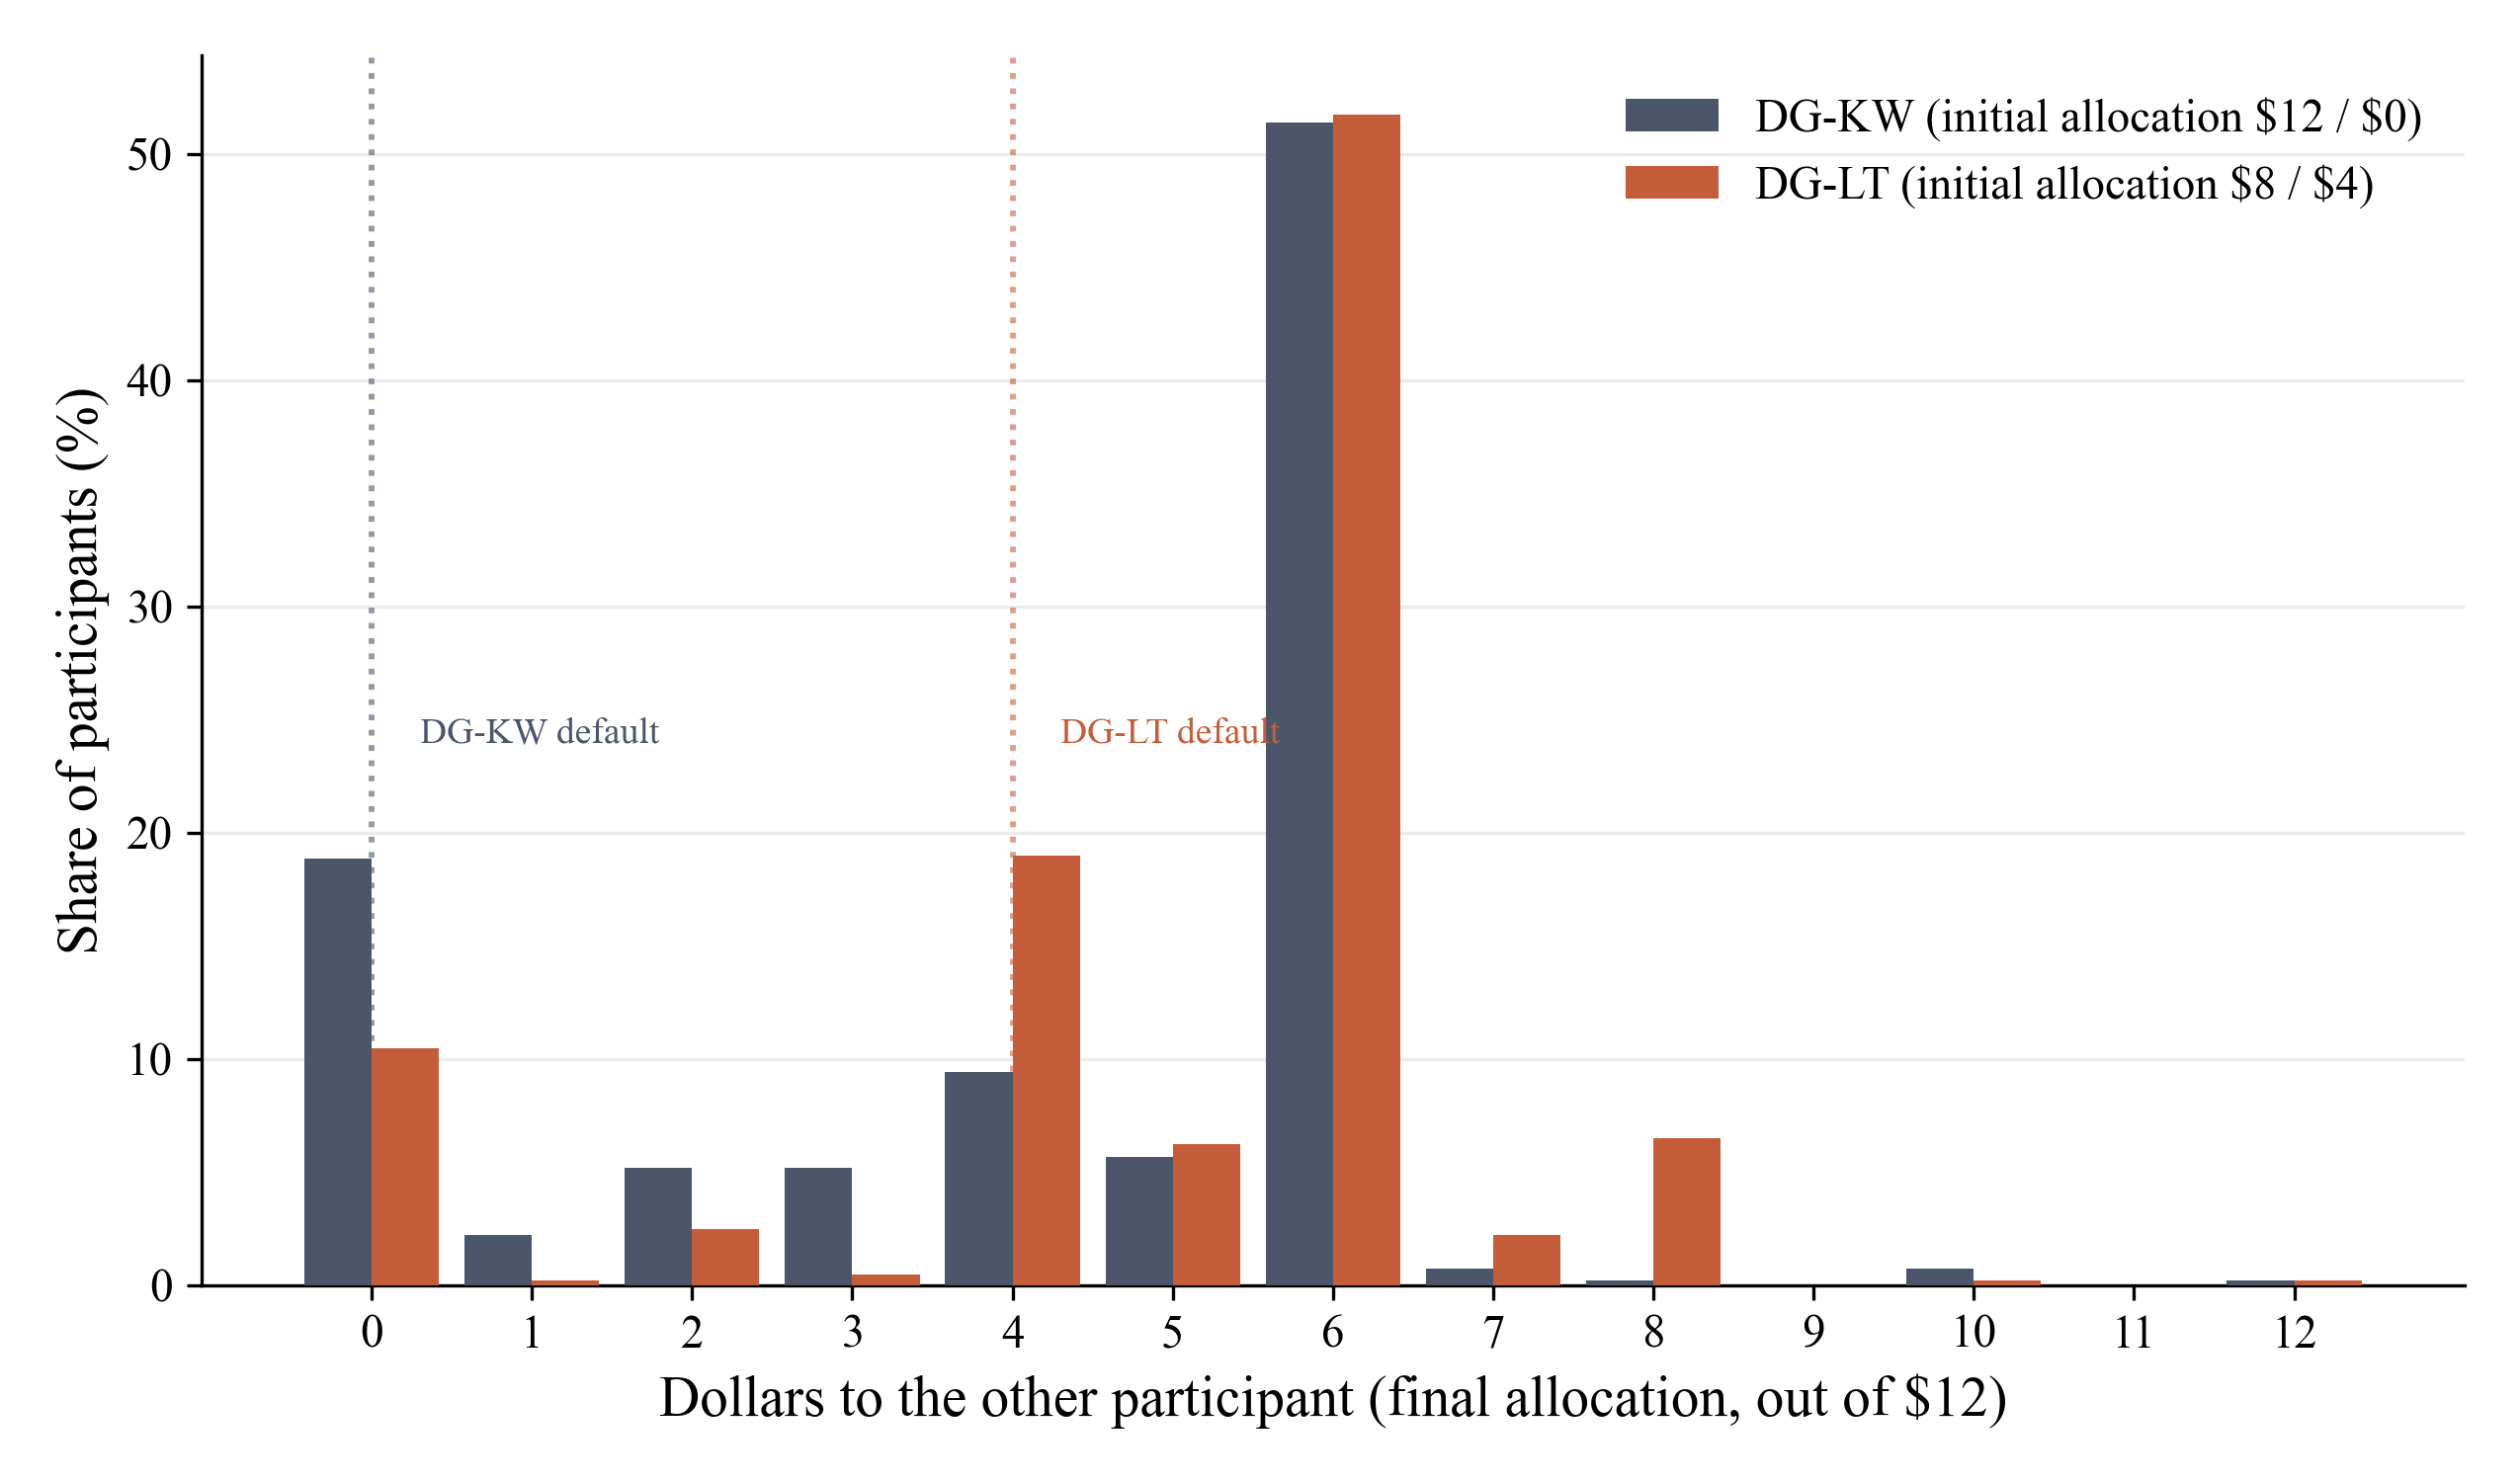
\includegraphics[width=0.9\textwidth]{intro_kw_vs_lt_control.png}
\caption{Final allocations to the other participant in two payoff-equivalent dictator games, control condition. In DG-KW the dictator is provisionally allocated \$12 and can transfer between \$0 and \$12; in DG-LT the provisional allocation is \$8/\$4 and the dictator can transfer between $-$\$4 and \$8. Dotted lines mark the default (no-transfer) allocation in each game. $N=403$ (DG-KW) and $N=400$ (DG-LT).}
\label{fig:intro_kw_lt}
\end{figure}

The leading account of such instability appeals to social norms.\footnote{The phenomenon is general: payoff-preserving expansions of the action set \citep{Bardsley2008}, hidden-information options \citep{DanaWeberKuang2007}, and costless exit \citep{LazearMalmendierWeber2012} all move behavior over unchanged alternatives.} \citet{KrupkaWeber2013} show that payoff-identical actions carry different degrees of social appropriateness in the two frames, and that elicited norms---combined with a stable preference for norm compliance---predict behavioral differences across dictator-game variants. This account is powerful but incomplete, in two ways. First, it measures the norm in each frame without explaining why minor, payoff-irrelevant changes move collectively shared judgments in the first place: the context-to-norm mapping remains a black box. Second, the instability lives \emph{within} the person, not only across frames. When the same participant plays both games of Figure~\ref{fig:intro_kw_lt}, nearly half change their choice (Appendix~\ref{app:within}): the same individual who shares generously under one description keeps under another, and any account built on stable individual traits---a taste for fairness, a fixed sensitivity to norms---records this instability without explaining it. \citet{FehrCharness2025} list the first gap among the central open questions in the social preferences literature; \citet{Camerer2003} flagged it two decades ago: framing effects are real, but ``the key step is figuring out what general principles (or theory of framing) can be abstracted'' from them. % chktex 12

This paper proposes and tests such a theory, building on the cognitive foundations developed by \citet{BordaloGennaioliLanzaniShleifer2026}. Before choosing, a player asks: \emph{what kind of situation is this?} She answers by matching the game, including its payoff-irrelevant contextual features, to similar situations she has experienced or can imagine---splitting a windfall with a friend, negotiating a price with a middleman, investing in a joint project \citep{Tversky1977, GilboaSchmeidler1995, BordaloGennaioliShleifer2012, BordaloCoffmanGennaioliShleifer2016, BordaloGennaioliShleifer2020}. The retrieved situation is the player's \emph{representation} of the game, and it directs attention to some payoff consequences over others. We formalize a representation as two objects retrieved together: attention weights over payoff elements---own earnings, total surplus, and a sharing norm---and beliefs about the other player's behavior. A representation says both what the game is about and whom one is facing. Given a representation, the player maximizes utility, so behavior inherits the instability of representations: contextual changes that shift which situation the game evokes shift norms, beliefs, and actions together, even though rules and payoffs are unchanged.

We test this account in a large pre-registered experiment on Prolific ($N \approx 12{,}750$ across roles and games) built around three classic games: the dictator game, the ultimatum game, and the trust game. The design has three ingredients. First, we \emph{measure representations directly}. After each decision, participants explain in open-ended text what drove their choice; a large language model, validated by human coders, classifies each answer into a Moral category (fairness, generosity, equality), a Self-interest category (own payoff), or a Mutual Benefit/Cooperation category (joint gains), alongside the social proximity of the counterpart the answer evokes. Second, we \emph{measure beliefs}: first movers in the ultimatum and trust games report the behavior they expect from the second mover, both in response to their chosen action and in response to a common reference action, which allows belief comparisons across participants who chose different actions. Third, we \emph{manipulate context while holding rules fixed}: relative to an abstract control, participants either play the same game framed as a market interaction between a data producer and a broker, or read and summarize a story about a workplace bonus or about charitable aid before playing the abstract game.

Four results emerge. First, absent any manipulation, representations vary systematically across games and predict behavior within each game. Moral representations dominate the dictator and ultimatum games but drop sharply in the trust game, where cooperative representations surge from near-absence to over a third of responses: the same subject pool spontaneously represents payoff-equivalent transfers in morally different ways depending on the strategic setting.\footnote{Moral shares are 68\%, 77\%, and 44\% of classified responses in the dictator, ultimatum, and trust games; Mutual Benefit/Cooperation rises from below 4\% in the first two to 37\% in the trust game.} Within games, categories predict actions as the attention weights imply---with a twist that only strategic structure explains: self-interested dictators transfer 10\% of the budget against 46\% for moral dictators, yet self-interested ultimatum proposers offer 42\%, close to the moral proposers' 50\%, because rejection risk disciplines low offers. In the trust game, cooperative senders send the most and hold the most optimistic beliefs about repayment. The two components of the representation are also linked as attention implies: moral proposers act on the norm regardless of what they expect, while self-interested proposers and senders track their beliefs.

Second, contextual manipulations shift representations and behavior coherently, and in ways that are hard to reconcile with context simply priming generosity or selfishness. The market frame crowds out moral representations in every game while raising both Self-interest and Mutual Benefit/Cooperation, and behavior follows the attention weights rather than a single ``market makes selfish'' direction: dictator giving and ultimatum offers fall, but trust-game sending \emph{rises}, together with markedly more optimistic beliefs about second movers.\footnote{Moral representations fall by 27, 43, and 24 percentage points in the dictator, ultimatum, and trust games; dictator giving falls by 11 percentage points and ultimatum offers by 22, while trust-game sending rises by 15.} Nor is this a shift in means alone: under the market frame the equal-split spike collapses while zero offers and full trust-game sends surge---mass moving between qualitatively different actions, the signature of a changed mixture of representations rather than of a single preference parameter sliding. The aid story, despite its charitable content, \emph{reduces} moral representations and increases self-interested ones relative to the bonus story in the dictator and ultimatum games, and it reduces giving; it leaves the trust game unaffected.

Third, representations quantitatively account for treatment effects. For each treatment comparison we estimate simple benchmark regressions of actions and beliefs on representation categories (and, where relevant, beliefs), and combine the estimated coefficients with the treatment-induced shifts in representations to \emph{predict} treatment effects. Predicted effects line up with actual effects across 18 outcome-by-comparison cells spanning both players and all games; predicted magnitudes fall short of actual ones, consistent with attenuation from coarse category measurement.\footnote{Regressing actual on predicted effects across the 18 cells yields $R^{2}=0.87$; predicted-to-actual ratios are near one half for the largest first-mover effects.} The same representation categories thus organize heterogeneity \emph{within} a context and instability \emph{across} contexts. Within-subject arms of the dictator experiment confirm the link at the individual level: participants whose representation changes across the two payoff-equivalent dictator games change their choice at more than twice the rate of those whose representation is stable (80\% versus 36\%).

Fourth, beliefs do not behave as rational expectations. Ultimatum proposers systematically underestimate acceptance in the abstract and story conditions (by roughly 16--17 percentage points) but swing to overestimation under the market frame. Under rational expectations, context could move beliefs only insofar as it moves behavior; instead, context moves beliefs through representations, and errors follow---with real allocative consequences, as the market frame's destruction of ultimatum surplus shows.

Our contribution is threefold. To the social preferences literature \citep{FehrSchmidt1999, BoltonOckenfels2000, CharnessRabin2002, FehrCharness2025}, we offer direct evidence on a mechanism that reconciles stable preferences with unstable behavior: what varies across contexts is not the taste for fairness but the representation that determines which motives receive attention. To the norms literature \citep{KrupkaWeber2013, KimbroughVostroknutov2016, Bicchieri2006, FehrSchurtenberger2018}, we supply the missing upstream step: norms shift across payoff-equivalent frames because frames change the situations games evoke, and we show the same mechanism operates in strategic games through beliefs, not only through injunctive judgments. The belief evidence also speaks to the literature on stated beliefs in games \citep{CostaGomesWeizsacker2008, ReyBiel2009}, where actions and elicited beliefs often fail to line up and the leading diagnosis is that subjects perceive the game differently across the two tasks: we measure that perception directly, and beliefs retrieved with the representation explain both when the two align and when they part ways.

To the literature on framing and context effects \citep{HoffmanMcCabeShachatSmith1994, LibermanSamuelsRoss2004, DufwenbergGachterHennigSchmidt2011, EckelGrossman1996, CherryFrykblomShogren2002}, we offer a unifying framework and a measurement strategy---open-ended reasoning classified at scale---that turns framing from a catalog of effects into a testable theory, in the spirit of \citet{BordaloGennaioliLanzaniShleifer2026}, who develop the cognitive machinery for individual decisions and explicitly point to games as the natural next application.\footnote{Related formal approaches include case-based decision theory \citep{GilboaSchmeidler1995} and analogy-based expectations \citep{Jehiel2005}, in which agents extrapolate from similar past cases or bundle games into analogy classes. Our contribution is empirical as much as theoretical: we measure the representation, not only its behavioral footprint.} The representational lens also carries welfare content: attention weights map directly into surplus and inequality (Section~\ref{sec:model_behavior}), so the same contextual shifts that move behavior have signed allocative consequences---under the market frame, destroying surplus in the ultimatum game while creating it in the trust game (Section~\ref{sec:ge}).

The paper proceeds as follows. Section~\ref{sec:model} presents the model: how a representation---attention together with beliefs---maps into behavior in the three games, and how context and experience determine which representation a game evokes. Section~\ref{sec:design} describes the experimental design, establishes the within-context results in the control sample, and measures the similarity structure that links our treatments to the theory. Section~\ref{sec:treatment} presents treatment effects on representations, actions, beliefs, and forecast errors, organized by the lever each treatment moves. Section~\ref{sec:ge} shows that representation shifts account for treatment effects, heterogeneity, and surplus, and returns to the motivating puzzle. Section~\ref{sec:discussion} concludes.

% ===== Section 2 rewritten along NG's skeleton (Representations_Games_NG_july9.docx). =====
% Equations follow NG's note of July 9; all derivations re-verified symbolically (sympy) on 2026-07-09.
% Corrections relative to the note: (i) solutions censored to [0,1]; (ii) d t^UG / d sigma < 0 holds
% UNCONDITIONALLY (NG's note conjectured it needed a sign condition on the numerator); (iii) the TG
% solution's "c" and "s" are the same object, and "t^UG" there should read "t^TG".
\section{Model}
\label{sec:model}

This section develops the framework in two steps. Section~\ref{sec:model_behavior} defines a representation---attention to payoff elements together with beliefs about the other player---and derives behavior taking the representation as given. Because the moral motive attaches to the sender's \emph{action} rather than to realized outcomes, the ultimatum and trust games reduce to \emph{modified dictator games}. Section~\ref{sec:determination} models where representations come from: a game description is matched, by similarity and by frequency of experience, to a category of situations, and the retrieved category slants the representation. This second step turns our two manipulations into theory-driven levers---the stories move the frequency with which a category is retrieved, the market frame moves the description itself---and it delivers the paper's organizing predictions: heterogeneity within a context, coherent shifts across contexts, and systematic forecast errors. A disparity-based alternative model that delivers the same core predictions is discussed in Appendix~\ref{app:theory_reconciliation}. Proofs of all propositions are in Appendix~\ref{app:proofs}.

\subsection{How Representations Shape Strategic Behavior}
\label{sec:model_behavior}

Two players interact once. Player $S$ is the first mover---the dictator, the proposer, the investor; generically, the \emph{sender}---and player $R$ is the second mover or \emph{receiver}. The sender's initial wealth is normalized to one, and her action is the share $t\in[0,1]$ she sends to the receiver. Total final wealth is $W(t)$, which may depend on the amount sent, $\pi_S$ denotes the sender's material payoff, and $\pi_R$ denotes the receiver's material payoff.

A \emph{representation} of the game is a pair $\mathbf{r}=(\boldsymbol{\alpha},\mathbf{x})$: an attention profile $\boldsymbol{\alpha}=(\rho,\sigma,\mu)$ over payoff elements and, in the strategic games, a believed behavior $\mathbf{x}$ of the receiver. Given her representation, the sender maximizes
\begin{equation}
u_S(t) \;=\; \rho\, W(t)\;-\;\sigma\, \pi_R\;-\;\frac{\mu}{2}\left(t-\tfrac12\right)^{2},
\label{eq:utility}
\end{equation}
where the three payoff elements are total wealth, the receiver's material payoff, and a sharing norm anchored at the equal split. The Greek letters are attention weights, with $\rho=\sigma=\mu=1$ the undistorted case in which no motive is slanted by the representation and the sender has inequity-averse utility in the spirit of \citet{BoltonOckenfels2000}. Standard models prescribe \emph{stability}---that is, an attention profile that stays fixed while context varies---and, in the strategic games, \emph{rational expectations}---that is, beliefs that track actual behavior. Because $\pi_S=W(t)-\pi_R$, equation~\eqref{eq:utility} can be rewritten as
\begin{equation*}
u_S \;=\; \sigma\,\pi_S \;+\; (\rho-\sigma)\,W(t)\;-\;\frac{\mu}{2}\left(t-\tfrac12\right)^{2},
\end{equation*}
which makes the mapping to motives transparent: $\sigma$ is attention to own earnings, $\rho-\sigma$ is attention to the total surplus over and above one's own share, and $\mu$ is attention to the norm. The functional form thus nests the motives of standard distributional preference models \citep{FehrSchmidt1999, BoltonOckenfels2000, CharnessRabin2002}, with two differences. First, the moral term is \emph{idealistic}: it attaches to what the sender does, not to what materializes afterwards. Whether the receiver accepts, rejects, or reciprocates, the sender has still sent the same $t$; only material payoffs are contingent on the other player's move. This assumption embodies a simple moral psychology---one feels right or wrong about one's own conduct---and it is what makes the strategic games tractable. Second, and central to everything that follows, beliefs are part of the representation rather than equilibrium objects: the process that determines what the game is \emph{about} also determines whom one imagines playing against. The attention weights and beliefs are properties of the situation the game evokes, not stable traits: the same person can be a moral dictator and a self-interested price-setter.

\paragraph{Dictator game.} Here $W(t)=1$ and $\pi_R=t$; there is no second mover to forecast, so $\mathbf{x}$ is empty.

\begin{proposition}[Dictator transfer]
\label{prop:dg}
The optimal transfer is $t^{DG}=\max\left\{0,\ \tfrac12-\tfrac{\sigma}{\mu}\right\}$. It never exceeds one half, is decreasing in the selfishness ratio $\sigma/\mu$, and is independent of $\rho$.
\end{proposition}

A moral representation (high $\mu$) anchors the transfer at the equal split; a self-interested one (high $\sigma$, low $\mu$) drives it to zero. A cooperative representation pins down $\rho$, which is idle in a fixed-pie game with no strategic margin: cooperative dictators act on their residual $\sigma/\mu$, which places them between the two poles when those residual weights are balanced. This matches the control-sample pattern of Figure~\ref{fig:control_outcomes}, where moral dictators transfer 46.2\% of the budget, self-interested dictators 10.3\%, and the (tiny) cooperative cell sits in between.

\paragraph{Ultimatum game.} If $R$ accepts, payoffs are as in the dictator game; if $R$ rejects, both players earn zero. The sender's representation now includes a believed behavior of the receiver, which we embed in an \emph{acceptance schedule}: the sender believes an offer $t$ is accepted with probability
\begin{equation*}
p(t)\;=\;a+b\,t, \qquad a,b>0,
\end{equation*}
so the belief component of her representation is the pair $\mathbf{x}=(a,b)$. Because the moral payoff is idealistic, only the material part of utility is scaled by acceptance, and the sender solves
\begin{equation}
\max_{t}\;\; p(t)\,\bigl(\rho-\sigma t\bigr)\;-\;\frac{\mu}{2}\left(t-\tfrac12\right)^{2}.
\label{eq:ug_objective}
\end{equation}

\begin{proposition}[Ultimatum offer]
\label{prop:ug}
The objective in~\eqref{eq:ug_objective} is strictly concave, and the optimal offer is
\begin{equation}
t^{UG}\;=\;\frac12\;+\;\frac{b\rho-(a+b)\,\sigma}{2b\sigma+\mu},
\label{eq:ug_offer}
\end{equation}
censored to $[0,1]$; the offer is interior if and only if $\bigl|b\rho-(a+b)\,\sigma\bigr|<b\sigma+\mu/2$. At an interior optimum: (i) if $p(1)=a+b\le 1$, then $t^{UG}>t^{DG}$ for every attention profile; (ii) the offer is increasing in $\rho$, decreasing in $\sigma$, and moved toward the equal split by $\mu$ (raised when $t^{UG}<\tfrac12$, lowered when $t^{UG}>\tfrac12$); (iii) the offer is decreasing in believed acceptance $a$, with sensitivity $\bigl|\partial t^{UG}/\partial a\bigr|=\sigma/(2b\sigma+\mu)$, which is increasing in $\sigma$ and decreasing in $\mu$.
\end{proposition}

Part (i) is the strategic discipline of the ultimatum game: because low offers risk rejection, \emph{every} representation offers more than it would transfer as dictator. This is why the enormous category gaps of the dictator game compress in the ultimatum game (46.2\% vs.\ 10.3\% becomes 50.0\% vs.\ 41.7\% in Figure~\ref{fig:control_outcomes}): the acceptance schedule disciplines precisely those senders whose own attention profile would otherwise push offers down. Part (iii) delivers two sharp empirical predictions. First, holding the representation fixed, offers should \emph{fall} with believed acceptance---a proposer who thinks low offers will be accepted makes them. Second, the belief sensitivity itself depends on attention: a moral (high-$\mu$) proposer acts on the norm regardless of what she expects, while a self-interested (high-$\sigma$) proposer tracks her beliefs. Both predictions are tested with our belief elicitation: the category-specific belief slopes of Section~\ref{sec:control} (Figure~\ref{fig:belief_sensitivity}) and the benchmark regressions of Section~\ref{sec:ge} bear both out. Attention to total wealth also acquires a role it lacks in the dictator game: $\partial t^{UG}/\partial\rho=b/(2b\sigma+\mu)$, which is strictly positive yet vanishes when acceptance is insensitive to the offer ($b=0$). The pie is fixed, but rejection destroys it, so weight on total wealth raises the offer purely through the fear of that destruction.
% DONE 2026-07-16: the sensitivity-by-category exhibit (NG's skeleton-3.2 ask, E1) is now Figure fig:belief_sensitivity in Section 3.2 + Table tab:belief_sensitivity in Appendix app:player2.

% MOVED 2026-07-13: the endogenous-acceptance-schedule Remark now lives in Appendix~app:receiver, per the AA+NG thread (main text keeps p(t) and s as primitives; formalization in appendix).
The acceptance schedule need not be taken as a primitive. Appendix~\ref{app:receiver} founds it in the receiver's own moral psychology---the offer's inequity is felt whether or not it is accepted, and rejection carries a psychological benefit of \emph{protest}---so the believed pair $(a,b)$ is a representation of the \emph{receiver's motives}, of how the sender perceives the receiver's representation: imagining a punitive receiver (our \emph{Moral bad} receiver category of Section~\ref{sec:design_details}) scales acceptance down across the board, while imagining a self-interested receiver makes acceptance sensitive to money. Under that foundation the condition $a+b\le 1$ in Proposition~\ref{prop:ug} also acquires a natural reading: the imagined receiver's protest weight is large enough that even a full-split offer is not certain to be accepted.

\paragraph{Trust game.} The amount sent is multiplied by $1+r$, with $r>0$ the net return, so total wealth is $W(t)=1+rt$.\footnote{In the experiment the multiplier is $m=1+r=3$ on a \$6 endowment, so $r=2$.} The sender believes the receiver returns a share $s$, with $0\le s<1$, of the multiplied amount $(1+r)t$, so the belief component of her representation is $\mathbf{x}=s$ and the receiver's believed material payoff is $\pi_R=(1-s)(1+r)t$.\footnote{We take the believed returned share to be constant for simplicity; like the acceptance schedule, it can be endogenized: Appendix~\ref{app:receiver} founds the return schedule in the receiver's moral psychology---a norm of returning half of a target pie---and shows that the comparative statics survive when the believed share declines in the send. % NG 2026-07-11: constant share maintained for the main analysis (NG's call); the output target is the tractable specification among the three candidates. Remark moved to Appendix app:receiver 2026-07-13 per the AA+NG thread.
} The sender solves
\begin{equation}
\max_{t}\;\;\rho\,(1+rt)\;-\;\sigma\,(1+r)\,t\,(1-s)\;-\;\frac{\mu}{2}\left(t-\tfrac12\right)^{2}.
\label{eq:tg_objective}
\end{equation}

\begin{proposition}[Trust send]
\label{prop:tg}
The optimal send is
\begin{equation}
t^{TG}\;=\;\frac12\;+\;\frac{\rho r-\sigma(1+r)(1-s)}{\mu},
\label{eq:tg_send}
\end{equation}
censored to $[0,1]$; the send is interior if and only if $\bigl|\rho r-\sigma(1+r)(1-s)\bigr|<\mu/2$. At an interior optimum, the send is increasing in $\rho$ and in the believed return share $s$ (with sensitivity $\sigma(1+r)/\mu$), decreasing in $\sigma$, and moved toward the equal split by $\mu$. As $\mu\to 0$ the problem becomes linear and the solution goes to a corner: a purely material sender sends everything if she believes the returned share exceeds the break-even level, $s(1+r)>1$, and nothing if it falls short. Finally, at interior optima, $t^{TG}\ge t^{DG}$ whenever $\rho\ge\sigma(1-s)$, with strict inequality unless $s=0$ and $\rho=\sigma$.
\end{proposition}

The trust game is where both components of the representation bite at once. Attention to total wealth is no longer idle: $\rho$ multiplies the return $r$, so cooperative senders---those who attend to the multiplied pie itself---send the most. Moral senders are anchored near the equal split (in the data, 44.1\%). Self-interested senders send the least unless they are optimistic, and their sends are the most belief-sensitive: as in the ultimatum game, the sensitivity $\sigma(1+r)/\mu$ rises with own-payoff attention and falls with moral attention. Whether the send sits above or below the equal split---the sign of the numerator in~\eqref{eq:tg_send}---is ambiguous: it is positive if and only if $\rho/\sigma>(1+r)(1-s)/r$, and for a purely material sender ($\rho=\sigma$) this reduces to the break-even condition $s(1+r)>1$, so the numerator is positive exactly when she believes trusting pays. The belief sensitivity $\sigma(1+r)/\mu$ holds at any interior optimum regardless of this sign (at a censored send it is locally zero). And in contrast to the ultimatum game, beliefs now enter with a \emph{positive} sign---optimism about the return raises the send, while optimism about acceptance lowers the offer. This sign flip across games is a distinctive joint prediction of the model, and the control-sample slopes of Figure~\ref{fig:belief_sensitivity}, like the benchmark regressions of Section~\ref{sec:ge}, confirm both signs. Table~\ref{tab:cs_summary} collects the comparative statics.

\begin{table}[!htbp]
\centering
\footnotesize
\renewcommand{\arraystretch}{1.2}
\caption{\textbf{Summary of Comparative Statics}}
\label{tab:cs_summary}
\begin{tabular}{l cccc c}
\toprule
& \multicolumn{4}{c}{Attention and beliefs} & Belief sensitivity \\
\cmidrule(lr){2-5}\cmidrule(lr){6-6}
Transfer & $\rho$ & $\sigma$ & $\mu$ & belief & $|\partial t/\partial \text{belief}|$ \\
\midrule
Dictator $t^{DG}$ & $0$ & $-$ & $\to\tfrac12$ & NA & NA \\
Ultimatum $t^{UG}$ & $+$ & $-$ & $\to\tfrac12$ & $-$ (acceptance $a$) & $\sigma/(2b\sigma+\mu)$ \\
Trust $t^{TG}$ & $+$ & $-$ & $\to\tfrac12$ & $+$ (return share $s$) & $\sigma(1+r)/\mu$ \\
\bottomrule
\end{tabular}
\begin{flushleft}
\footnotesize Notes: Signs at interior optima; solutions are censored to $[0,1]$. ``$\to\tfrac12$'' means the moral weight moves the transfer toward the equal split, so over the empirically relevant range ($t<\tfrac12$) its effect is positive. In each game the belief sensitivity is increasing in $\sigma$ and decreasing in $\mu$: self-interested representations track beliefs, moral representations act on the norm.
\end{flushleft}
\end{table}
% RESOLVED 2026-07-13 (was NOTE 2026-07-11, NG Commento 1 "poi"): SN decision --- section inserted below, ported verbatim from model-2.tex "Welfare and Inequality" (only the two "in the paper" pointers adapted to \ref{sec:forecast}/\ref{sec:heterogeneity}); proofs in app:proofs. Self-contained; moves with a clean cut if the call decides otherwise.

\paragraph{Welfare and inequality.}
The comparative statics about the sender's action immediately deliver comparative statics for total surplus and for the division of payoffs, which is where representations acquire social content. Let $V_g$ denote expected total material wealth at an interior optimum---$V_{DG}=1$, $V_{UG}=p(t^{UG})$ (the pie survives only if the offer is accepted), $V_{TG}=1+r\,t^{TG}$---and let $D_g=\pi_S-\pi_R$ denote the payoff gap conditional on trade (in the ultimatum game, given acceptance; the other games have no rejection margin).

\begin{proposition}[Welfare]
\label{prop:welfare}
At interior optima: (i) surplus attention raises welfare where the pie responds to the action, with strength quadratic in that response: $\partial V_{DG}/\partial\rho=0$, $\partial V_{UG}/\partial\rho=b^{2}/(2b\sigma+\mu)$, $\partial V_{TG}/\partial\rho=r^{2}/\mu$; (ii) own-payoff attention destroys welfare in both strategic games, $\partial V_{UG}/\partial\sigma=-b\bigl[(a+b)\mu+2b^{2}\rho\bigr]/(2b\sigma+\mu)^{2}<0$ and $\partial V_{TG}/\partial\sigma=-r(1+r)(1-s)/\mu<0$, and unambiguously lowers the counterpart's expected payoff; the sender's own expected payoff can fall as well, precisely when $b(1-2t^{UG})>a$---a steep believed schedule with a low intercept; (iii) in the strategic games, norm attention raises welfare exactly when the material pull is selfish---$\partial V_{g}/\partial\mu$ has the sign of $\tfrac12-t^{g}$---while dictator-game welfare is unaffected by any weight; (iv) optimism raises welfare: $\partial V_{UG}/\partial a=(b\sigma+\mu)/(2b\sigma+\mu)>0$ and $\partial V_{TG}/\partial s=r\sigma(1+r)/\mu>0$.
\end{proposition}

Part (i) formalizes cooperation through attention: a sender who attends to total wealth gives more precisely where giving protects (ultimatum) or produces (trust) the pie, and welfare rises with the \emph{square} of the pie's sensitivity to the action, because attention moves the action by that sensitivity and the action moves the pie by it again. Part (ii) is the reverse face: own-payoff attention is socially destructive in every strategic game, and it is not even reliably self-serving---when rejection risk is steep, the offer cut costs more in expected acceptance than it saves in shares. Part (iii) says the norm is a social technology against selfish material pulls, not a complement to cooperative ones: when the pull is generous (an optimistic cooperator in the trust game), the anchor drags the send back toward one half and destroys surplus.

These statements evaluate the ultimatum pie at the sender's own beliefs: $V_{UG}=p(t^{UG})$ is expected surplus under her model of the world. This is by design---a rational-expectations welfare measure would impose exactly the belief--behavior alignment the data reject---and the ultimatum game is the only place where the choice matters: dictator surplus is constant, and trust surplus $1+r\,t^{TG}$ is belief-free given the send, with the division evaluated at the actual share below.

\begin{remark}[Believed versus Realized Welfare]
\label{rem:realized}
Let actual acceptance follow any increasing, differentiable schedule $\hat p$, held fixed as the sender's parameters vary, and let $\hat V_{UG}=\hat p(t^{UG})$ denote realized expected surplus at the offer chosen under the believed schedule. Parts (i)--(iii) of Proposition~\ref{prop:welfare} survive with the same signs: attention weights enter neither schedule, so they move realized surplus only through the action, $\partial\hat V_{UG}/\partial\theta=\hat p'(t^{UG})\cdot\partial t^{UG}/\partial\theta$ for $\theta\in\{\rho,\sigma,\mu\}$, and only magnitudes change. Part (iv) reverses in the ultimatum game: optimism no longer raises acceptance directly---it only lowers the offer, and actual acceptance falls with it---so $\partial\hat V_{UG}/\partial a<0$; its trust-game half is unchanged.
\end{remark}

Believed and realized welfare thus part ways exactly where beliefs and behavior do---an optimistic proposer expects more surplus and produces less---which is the forecast-error mechanism of Section~\ref{sec:forecast} behind the ultimatum-game surplus accounting of Section~\ref{sec:heterogeneity}.

\begin{proposition}[Inequality]
\label{prop:inequality}
Conditional on trade, $D_{DG}=2\sigma/\mu$ and $D_{UG}=2\bigl[(a+b)\sigma-b\rho\bigr]/(2b\sigma+\mu)$: own-payoff attention widens the gap, surplus attention narrows it (strictly in the ultimatum game), and norm attention compresses it toward zero, $\partial D_{UG}/\partial\mu=-D_{UG}/(2b\sigma+\mu)$ and $\partial D_{DG}/\partial\mu=-D_{DG}/\mu$. In the trust game, for an actual returned share $s_{a}$, $D_{TG}=1-t\bigl[1+(1+r)(1-2s_{a})\bigr]$: a larger send narrows the gap if and only if $s_{a}<(2+r)/\bigl(2(1+r)\bigr)$, and norm attention compresses the gap toward its equal-split value $\bigl[1-(1+r)(1-2s_{a})\bigr]/2$, which is zero only at $s_{a}=r/\bigl(2(1+r)\bigr)$.
\end{proposition}

The norm anchor coincides with payoff equality in the fixed-pie games but not, in general, in the trust game: with $r=2$---the experiment's tripling of the send---the equal-split send equalizes payoffs only if the receiver returns exactly one third of her output. The population reading connects these statics to the treatments: a treatment that reweights retrieved categories toward high-$\sigma$, low-$\mu$ representations in the ultimatum game destroys expected surplus and widens conditional inequality, while one that reweights toward high-$\rho$ representations and optimistic beliefs in the trust game creates surplus---the pattern of the surplus accounting in Section~\ref{sec:heterogeneity}.

\paragraph{From measured categories to model parameters.}
\label{sec:mapping}
Our empirical categories map onto the representation as follows. A \textbf{Moral} representation (fairness, generosity, equality) corresponds to high norm attention $\mu$. A \textbf{Self-interest} representation corresponds to high own-earnings attention---$\sigma$ high with $\rho\approx\sigma$, since own earnings are $\sigma\pi_S$ when the surplus weight $\rho-\sigma$ is nil---and low $\mu$. A \textbf{Mutual Benefit/Cooperation} representation (joint gains, teamwork) corresponds to surplus attention, $\rho>\sigma$. For second movers, the protest foundation of Appendix~\ref{app:receiver} distinguishes \textbf{Moral good} (fairness, reciprocity: $\hat\rho>\hat\sigma$ with moderate protest weight) from \textbf{Moral bad} (condemnation of the sender: a high protest weight, hence rejection), with \textbf{Self-interest} making acceptance money-sensitive and returns low. The belief components $(a,b)$ and $s$ are measured directly by the belief and hypothetical-belief questions. The model does not restrict how $\mathbf{x}$ relates to $\boldsymbol{\alpha}$ across people: beliefs may be anchored on a commonly held standard (as we find in the ultimatum game, where believed acceptance is flat across categories) or may covary with own attention, as under \emph{projection}---a cooperative sender imagining a cooperative receiver (as we find in the trust game). Which regime prevails is an empirical question that Section~\ref{sec:control} answers game by game.
% TODO (NG Commento 3, 2026-07-11): calibration of (rho/mu, sigma/mu) per category from control moments is worked out in model-2.tex ("From Measured Categories to Model Parameters"). First pass from audited v1 moments (r=2): Self-interest sigma/mu=0.397, rho/mu=0.362 (the rho~sigma mapping emerges from the data); implied UG schedule a=0.26, b=0.67 (valid: a+b=0.93<=1); Moral sigma/mu=0.038, norm-dominated, (a,b) unidentified exactly as its own insensitivity implies; MBC locus has rho>sigma for all admissible sigma/mu; predicted-vs-E1 sensitivities show a common ~2.5x attenuation (UG 0.26 vs 0.10; TG 1.19 vs 0.47). AA 2026-07-11: prefer the two-point route --- hypothetical + chosen-action beliefs identify (a,b) from measurement alone, the UG FOC becomes an overidentifying test, and Moral's schedule is identified too; full spec = E6 in exhibit_specs_v2.md (E7 there = AA's joint-distribution independence counterfactual). Paper placement (Section 5?) to decide at the call.
% NOTE 2026-07-12 (AA punto 1, endorsed by NG: "vale la pena guardarci"): exact model result for E7 now in model-2.tex, Remark "Joint Distribution of Attention and Beliefs" (rem:joint) --- at interior optima the TG mean send is bilinear in (sigma/mu, s), so the gap vs the independent-marginals counterfactual is EXACTLY E[t]-E_indep[t] = (1+r)*Cov(sigma/mu, s); rho/mu enters linearly, so no other covariance moves the mean. No closed form in the UG (b enters the denominator 2b*sigma+mu --- gap computed numerically; predicted ~0 with acceptance beliefs flat across categories) nor under the declining schedule s(t)=s0-s1*t (exact only at s1=0). Under projection Cov<0 --- mean TG sends BELOW independence, the E7 prediction as a displayed formula. Verified symbolically in ng_reply_round2_checks.py (root). NG's "non mi pare ci sia forte correlazione tra attention e beliefs" is the UG regime (common standard); the TG is where the coupling must bite (22.0/31.5/35.7 beliefs by category). E7 spec updated; paper slot for E7 still a call decision.

Three testable rankings and two belief-channel signs follow. Transfers should rank Moral $>$ Self-interest in the dictator game with a wide gap; the gap should compress in the ultimatum game; sends should rank Mutual Benefit/Cooperation $>$ Moral $>$ Self-interest in the trust game. Offers should fall with believed acceptance in the ultimatum game; sends should rise with the believed return in the trust game. And the action--belief sensitivity should be strongest for Self-interest representations in both strategic games, since it is increasing in $\sigma$ and decreasing in $\mu$.

\begin{remark}[Relation to a disparity-based model]
\label{rem:reconciliation}
An alternative model---developed in a companion Model Appendix---replaces the action-based norm with an outcome-based disparity cost $(y_S-y_R)^2$ and treats beliefs as point forecasts of the receiver's attention weights rather than as primitives. The motive triad is the same ($\sigma\leftrightarrow$ own earnings, $\rho-\sigma\leftrightarrow$ efficiency, $\mu\leftrightarrow$ norm/disparity), and the core predictions coincide: dictator transfers ranked by category and capped at one half, ultimatum offers above dictator transfers and compressed across categories by strategic discipline, trust driven by efficiency attention and gated by optimism. The models differ in mechanics---censoring at a believed minimum acceptable offer versus a smooth acceptance schedule---and in a handful of secondary predictions. Appendix~\ref{app:theory_reconciliation} records the correspondence.
\end{remark}

\subsection{How Representations Are Determined}
\label{sec:determination}

The sender does not see a game form; she sees a \emph{description} $\mathbf{d}=(\mathbf{r}_d,\boldsymbol{\kappa}_d)$, where $\mathbf{r}_d$ is the representation implied by a literal reading of the rules and $\boldsymbol{\kappa}_d$ is the context: the labels, the cover story, the setting in which the interaction is embedded. Her memory contains \emph{categories} of experience $c\in\mathbf{C}$---classes of situations she has lived or can imagine, such as sharing a windfall, haggling over a price, investing in a joint project---each with a typical representation $\mathbf{r}_c$, a typical context $\boldsymbol{\kappa}_c$, and a time-weighted frequency $F_c$ \citep{BordaloGennaioliShleifer2020, BordaloGennaioliLanzaniShleifer2026}. Facing the description, she selects a category and a representation $\mathbf{r}=(\boldsymbol{\alpha},\mathbf{x})$ to solve
\begin{equation}
\max_{c\in\mathbf{C},\,\mathbf{r}\in\mathbf{R}}\;\;F_c\cdot S\bigl[(\mathbf{r},\boldsymbol{\kappa}_d),(\mathbf{r}_c,\boldsymbol{\kappa}_c)\bigr]\;+\;S\bigl[(\mathbf{r},\boldsymbol{\kappa}_d),(\mathbf{r}_d,\boldsymbol{\kappa}_d)\bigr]\;+\;\epsilon_c,
\label{eq:retrieval}
\end{equation}
where $S$ is a similarity function \citep{Tversky1977, GilboaSchmeidler1995} and $\epsilon_c$ is an i.i.d.\ extreme-value shock. The chosen representation trades off fidelity to the description (the second term) against assimilation to the best-fitting category of experience (the first term).
% RESOLVED 2026-07-11: eq:retrieval is structurally BGLS (2026) eq. (20), the description-augmented recognition problem --- F_c = sum_{tau in c} delta^(t-tau) (their fn. 7), unit-weight fidelity = their present-description term, epsilon_c/logit = their Prop. 2 (interference = the softmax denominator, distinct from fidelity), cue-strength refinement = their contrast weights sigma with the sigma_c F_c / sigma_delta threshold (their eq. 22). Substantive differences (= the games contribution): attended features are payoff elements with weights that can exceed 1, and beliefs are prototype content, not distortions of a known P (no objective distribution over the counterpart in a one-shot game) --- which is what makes forecast errors possible. Full mapping in model-2.tex, section "Relation to BGLS (2026)". RESOLVED 2026-07-13 (SN): departures stated explicitly --- condensed relation paragraph inserted below, before the three implications; notation stays ours. Remaining NG call: only whether to adopt the eq. 22 contrast-weight machinery, now specced as an optional module in similarity_survey_design.md, where it has operational content.

Equation~\eqref{eq:retrieval} has two forces, and each of our manipulations targets one of them. First, a higher frequency $F_c$ fosters a category's retrieval, increasing the likelihood that the sender slants her representation toward $\mathbf{r}_c$, \emph{for a given description}. This is the \textbf{story lever}: reading and summarizing a story about a workplace bonus or about charitable aid is a recent, vivid experience that raises the retrieval weight of its category, while the description of the game itself is unchanged. Second, a change in the context $\boldsymbol{\kappa}_d$ that makes the description more similar to the contexts $\boldsymbol{\kappa}_c$ of experiences in some category also fosters that category's retrieval, \emph{for given frequencies}. This is the \textbf{frame lever}: describing the identical game as a transaction between a data provider and a broker moves the description itself into the neighborhood of market experiences.

The frequency weight has a natural recency structure. Let each experience $e$ in category $c$ have age $\tau_{e}$ and let $F_{c}=\sum_{e\in c}\delta^{\tau_{e}}$ with $\delta\in(0,1)$: frequency is experience discounted by recency. The description just read is then itself the most recent trace---age zero, weight $\delta^{0}=1$---which is why fidelity carries a fixed unit weight in equation~\eqref{eq:retrieval}: both terms are recency-weighted similarities. This reading disciplines the trade-off between memory and description. A story is an age-zero experience added to its category, so a single story can rival a lifetime of discounted experience---which is why the story lever works at all; and when discounting is strong every $F_{c}$ is small, so the description dominates and memory cannot drown it unless a category is both frequent and recent. A natural refinement scales fidelity by a cue-strength parameter increasing in the description's distinctiveness---its dissimilarity from the stored contexts---so that a description unlike anything in memory resists assimilation.

Equation~\eqref{eq:retrieval} is not bespoke. It is, structurally, the description-augmented recognition problem of \citet{BordaloGennaioliLanzaniShleifer2026} (their equation~20): the chosen representation plays the role of their tuned attention vector; category prototypes and their recency-weighted frequencies $F_c$ are defined exactly as theirs; fidelity to the description enters without a frequency multiplier in both frameworks (the present description is the age-zero trace); and the extreme-value shock delivers their logit retrieval probabilities. Their results transfer: attention tunes to the retrieved category and neglects discrepant context, which makes categorization sticky, and a change in a feature's bottom-up salience can re-categorize the problem---their theory of framing is our frame lever. Two departures are deliberate, and they are the games contribution. First, the attended features here are the payoff elements of a strategic problem rather than those of a known lottery: their bound $\alpha\in[0,1]$ shades perceived values relative to true ones, while here no veridical attention profile exists---behavior identifies only relative weights, and the undistorted case $\rho=\sigma=\mu=1$ is a statement about ratios, not levels. Second, beliefs: in their framework perceived probabilities are attention-distortions of an objective distribution, but in a one-shot game there is no objective distribution over the counterpart to distort---the category supplies the belief itself, the imagined receiver $(a,b)$ or $s$ as prototype content. This is the model's one genuinely new retrieval object, and it is what makes systematic forecast errors possible: the third implication below. They close by listing strategic behavior as a natural application of problem recognition; the model of this section is that application.

Three implications organize the empirical work.
\begin{enumerate}
\item \emph{Heterogeneity within a context.} Within a treatment, people hold different representations (they have different histories $F_c$ and draw different shocks $\epsilon_c$), so behavior is heterogeneous, and its heterogeneity is structured by the mixture of retrieved categories, not merely by noise. % DONE 2026-07-16: measured as the between/within-category variance decomposition, Table tab:heterogeneity_decomposition in Section 5.1 (E3; variance/skewness moments demoted to robustness per NG).
\item \emph{Instability across contexts.} Across treatments, the distribution of retrieved categories shifts---through $F_c$ for the stories, through $\boldsymbol{\kappa}_d$ for the market frame---and the action moves in the direction that \emph{combines} the attention differences (across $\boldsymbol{\alpha}$) and the belief differences (across $\mathbf{x}$) of the categories gaining and losing weight. Holding category-typical actions fixed, the mean effect of a manipulation is the composition change $\Delta E[t^{g}]=\sum_{c}\Delta q_{c}\,\bar{t}_{c}^{\,g}$, where $q_{c}$ is the retrieval probability of category $c$ and $\bar{t}_{c}^{\,g}$ its typical action in game $g$: the product of a retrieval shift, whose size is gated by the similarity between the game's description and the manipulated content, and the spread of category-typical actions in that game. Both factors are game-specific and measurable, so the same manipulation can move one game strongly and another barely at all---not because any payoff element drops out of the representation, but because retrieval shifts less where similarity is low and matters less where the retrieved categories act alike. Heterogeneity and instability are two faces of the same object.
\item \emph{Forecast errors and learning.} Nothing in~\eqref{eq:retrieval} guarantees that the two players' representations are shared or mutually consistent: the sender's imagined receiver is retrieved from the sender's memory, not from the receiver's behavior. Systematic, context-dependent forecast errors are therefore an equilibrium object of the theory, not a pathology---and learning in games under a stable context can be read as convergence toward representations that no longer generate salient surprises, which is what renders equilibria stable.\footnote{Appendix~\ref{app:receiver} formalizes this extension: the receiver faces a richer description that includes the sender's action, so her retrieval is cued by the offer itself; aggregate acceptance and return schedules are retrieval mixtures of category schedules, and a treatment that moves the two players' descriptions differently moves mean forecast errors. % RESOLVED 2026-07-13 (AA+NG thread): formalization placed in Appendix app:receiver, one-sentence pointers in the text.
}
\end{enumerate}

The theory's inputs are, in principle, measurable: the similarity of our contexts to broad categories of experience---cooperation problems, conflict problems, moral problems---and to receiver types who accept or reject, return or keep. Section~\ref{sec:similarity} reports a first pass at such measurement and uses it to discipline the interpretation of the treatments; a human-subjects similarity survey is in progress. % TODO: field the similarity survey (design in similarity_survey_design.md).

\section{The Experiment}
\label{sec:design}

This section proceeds in three steps. It first describes the experimental design and measurement (Section~\ref{sec:design_details}). It then uses the control sample to establish the empirical content of the representation measure: how stated categories vary across games and relate to actions and beliefs (Section~\ref{sec:control}). Finally, it examines the similarity structure that links the treatments to the retrieval model (Section~\ref{sec:similarity}).

\subsection{The Protocol}
\label{sec:design_details}

\paragraph{Games and roles.} Participants, recruited on Prolific, are randomly assigned to one of three canonical games \citep{ForsytheHorowitzSavinSefton1994, GuthSchmittbergerSchwarze1982, BergDickhautMcCabe1995}---DG, UG, or TG---to one role, and to one of the four conditions below. In the DG and UG the budget is \$12; in the TG the sender's endowment is \$6 and the multiplier is $m=3$. To make decisions consequential while keeping the sample large, the chosen allocation is implemented for one participant (pair) in ten. In the main text we focus on the KW version of the dictator game (provisional allocation \$12/\$0) and on first movers (Player 1); the LT version (\$8/\$4 with a take option) appears in the Introduction, enters the similarity gradient of Section~\ref{sec:aid_bonus} and the dispersion accounting of Section~\ref{sec:heterogeneity}, and returns in Section~\ref{sec:kwlt}; second movers (Player 2) return in Section~\ref{sec:ge}, with full detail in Appendix~\ref{app:player2}. Deferring second movers is a matter of identification, not of importance: their clean comparisons require the hypothetical responses at fixed actions described below, and Section~\ref{sec:ge} reports them and folds both players into the accounting exercise.

\paragraph{Conditions.} We compare four conditions that hold rules, action sets, and payoff consequences fixed:
\begin{itemize}
\item \textbf{Control}: the game in abstract framing (``you and your match are provisionally allocated a certain amount of dollars\ldots'').
\item \textbf{Market}: the same game framed as a market interaction. The first mover is a \emph{data provider} who sets the price of her data; the second mover is a \emph{broker} who resells it to the research team (and, in the UG, can reject the price; in the TG, can transfer revenue back). Roles, action sets, and payoffs are identical to Control.
\item \textbf{Bonus}: before playing the abstract game, participants read and summarize a story about a team leader deciding whether to share a performance bonus with a teammate.
\item \textbf{Aid}: before playing the abstract game, participants read and summarize a story about a welfare recipient deciding whether to share unexpected financial aid with a struggling neighbor.
\end{itemize}
The stories manipulate which real-world situation the game evokes without mentioning the game itself; the market frame manipulates the description of the interaction directly. Instructions and stories are reported in Appendix~\ref{app:instructions}. Our two pre-registered comparisons are \textbf{Market vs Control} and \textbf{Aid vs Bonus}; the latter holds constant the presence of a story and varies only its content.\footnote{The experiments were pre-registered on AsPredicted: \#261370 (dictator games, including the within-subject arms analyzed in Appendix~\ref{app:within} and the hypothetical-allocation representation measure analyzed in Appendix~\ref{app:hp}) and \#286187 (ultimatum and trust games, including belief elicitation and its accuracy). Pre-registered sample sizes are 400 participants per between-subject dictator cell plus 600 per within-subject arm, and 600 participants per role in each ultimatum/trust cell; participants failing an attention check or twice failing comprehension questions are screened out. The final Player 1 sample comprises 1,604 (DG-KW), 1,603 (DG-LT), 2,400 (UG), and 2,400 (TG) observations; the Player 2 sample comprises 2,402 (UG) and 2,346 (TG). Trust-game receivers are recruited only for senders who send a positive amount, which is why fewer than 2,400 were fielded.}

\paragraph{Measuring representations.} We measure representations in the most direct way available: by asking participants to describe them. After choosing, each participant answers an open-ended question about what drove her decision (the ``reasons'' question). Free text does not force participants into categories chosen by the analyst, and it can be collected at scale.\footnote{Open-ended elicitation and automated text classification are an emerging measurement strategy in economics \citep{FerrarioStantcheva2022, HaalandRothStantchevaWohlfart2024}; here they are deployed inside incentivized games and tied to a model of retrieval.} Following the pre-registered procedure, a large language model (GPT-4.1) classifies each answer---with classification rules validated by human coders\footnote{Human coders classified 3,990 responses in six validation subsamples: for each classification batch (Player 1 in the story arms, Player 1 in Market and Control, Player 2 in all four arms), two disjoint subsamples drawn stratified on the LLM-assigned category, with roughly 100 responses per game--arm cell. Two research assistants---each responsible for one subsample throughout, and blind to the treatment arm and to the game---applied the same written classification rules given to the LLM\@. Human--LLM agreement is 76\% overall (Cohen's $\kappa=0.64$): 80\% ($\kappa=0.63$) and 79\% ($\kappa=0.69$) in the two Player-1 batches, and 71\% ($\kappa=0.57$) for Player 2, whose five-category scheme is finer; there, disagreements concentrate at the \emph{Moral good}/\emph{Mutual Benefit} boundary. Appendix~\ref{app:validation} reports rates by subsample and arm.}---into one of three substantive categories for Player 1 (\emph{Moral}, \emph{Self-interest}, \emph{Mutual Benefit/Cooperation}) and four for Player 2 (\emph{Moral good}, \emph{Moral bad}, \emph{Self-interest}, \emph{Mutual Benefit/Cooperation}), plus a residual \emph{No clear justification} (henceforth ``unclassified'').\footnote{The residual category accounts for 1--3.5\% of control responses. The classification also codes the \emph{social proximity} of the counterpart evoked by the answer (no mention, abstract stranger, anonymous peer, teammate/coworker, friend). Appendix~\ref{app:hp} reports a second, pre-registered representation measure based on participants' descriptions of real-world situations similar to hypothetical final allocations; the two measures deliver consistent conclusions.}
% DONE 2026-07-10 via 06_validation_and_within_checks.py from missingdata/ (AA delivery): agreement footnote above + Table tab:llm_human_agreement in new Appendix app:validation.
% DONE 2026-07-10 (AA reply, rounds 2-3): protocol confirmed --- classifier GPT-4.1, prompt = the written classification rules (word file); two RA coders, one per subsample throughout, blind to treatment and game; subsamples drawn stratified on the LLM category. Blindness to the participant's chosen AMOUNT not explicitly confirmed --- not claimed in the text.
We treat the assigned category as a (noisy, discrete) measure of the participant's representation---the attention profile $\boldsymbol{\alpha}$ of Section~\ref{sec:mapping}---and three features of the data support this reading. First, categories are not relabeled actions. If participants merely described their choice in words, a given category would map onto similar behavior wherever it appears; instead, the same category maps onto the behavior the strategic structure dictates: self-interested proposers offer four times what self-interested dictators transfer, because an offer must survive the responder's acceptance decision while a dictator faces no such constraint. A verbal copy of the action could not produce this pattern; a motive filtered through the rules of the game does. Second, categories predict beliefs about the \emph{other} player at a fixed reference action, an object that no rationalization of one's own choice pins down. Third, a second pre-registered measure, elicited \emph{before} the decision and anchored to hypothetical allocations rather than to the choice, delivers the same cross-game and treatment patterns (Appendix~\ref{app:hp}): whatever the categories capture is present before the action is taken. The residual caveat is that reasons are elicited after the choice, so category--behavior associations could partly reflect ex-post rationalization of the chosen action; the three features above bound that concern, and we flag it where it bites. A standing language rule follows from the design: throughout the paper, effects of the randomized context manipulations are causal; relationships between categories and behavior are associations, since categories are measured rather than assigned.

\paragraph{Measuring beliefs.} First movers in the UG report the probability that their offer is accepted; in the TG, the amount they expect back. We call these \emph{chosen-action beliefs}. Because they condition on endogenously chosen actions, we also elicit \emph{hypothetical beliefs} at a common reference action---the probability that an offer of one third would be accepted, and the expected return to sending one third---which are comparable across participants and treatments. Second movers report both their response to the matched first mover's actual action and their responses to hypothetical actions, including the same one-third reference. In the language of the model, the reasons question measures the attention component $\boldsymbol{\alpha}$ of the representation and the belief questions measure its believed-behavior component $\mathbf{x}$; we elicit hypothetical beliefs at a fixed action precisely because $\mathbf{x}$ is a \emph{function}, and second movers' hypothetical responses trace the same function from the other side.

\subsection{Representations and Sender Behavior in Control}
\label{sec:control}

The control sample establishes four descriptive facts. Stated representation categories differ across games, both in what participants emphasize and in the counterpart they evoke; they are associated with actions and with beliefs; and the action--belief relationship itself varies across categories. The model of Section~\ref{sec:model} provides a unified interpretation of these patterns.

\paragraph{Representations differ across games.} The same population, playing for stakes of comparable magnitude, spontaneously represents the three games in morally different ways. Figure~\ref{fig:control_cats} shows the distribution of Player 1 categories in the control condition, by game. In the two fixed-pie games moral reasoning dominates---68.4\% of classified DG-KW responses and 76.6\% of UG responses---while in the TG the picture changes discretely: Moral falls to 43.8\% and Mutual Benefit/Cooperation, negligible in the DG-KW and the UG (0.8\% and 3.3\%), rises to 37.0\%.\footnote{Self-interest varies much less across games: 30.8\%, 20.1\%, and 19.2\% in the DG-KW, UG, and TG\@. One procedural asymmetry qualifies the cross-game comparison: dictator-game participants completed the hypothetical-allocation task of Appendix~\ref{app:hp} before choosing, while UG and TG participants did not.} Only the strategic structure differs across these games, and with it the situations they evoke: the multiplier and the sequential exchange of the TG evoke joint production; the fixed pie of the DG and UG evokes sharing and its ethics.
\begin{figure}[!htbp]
\centering
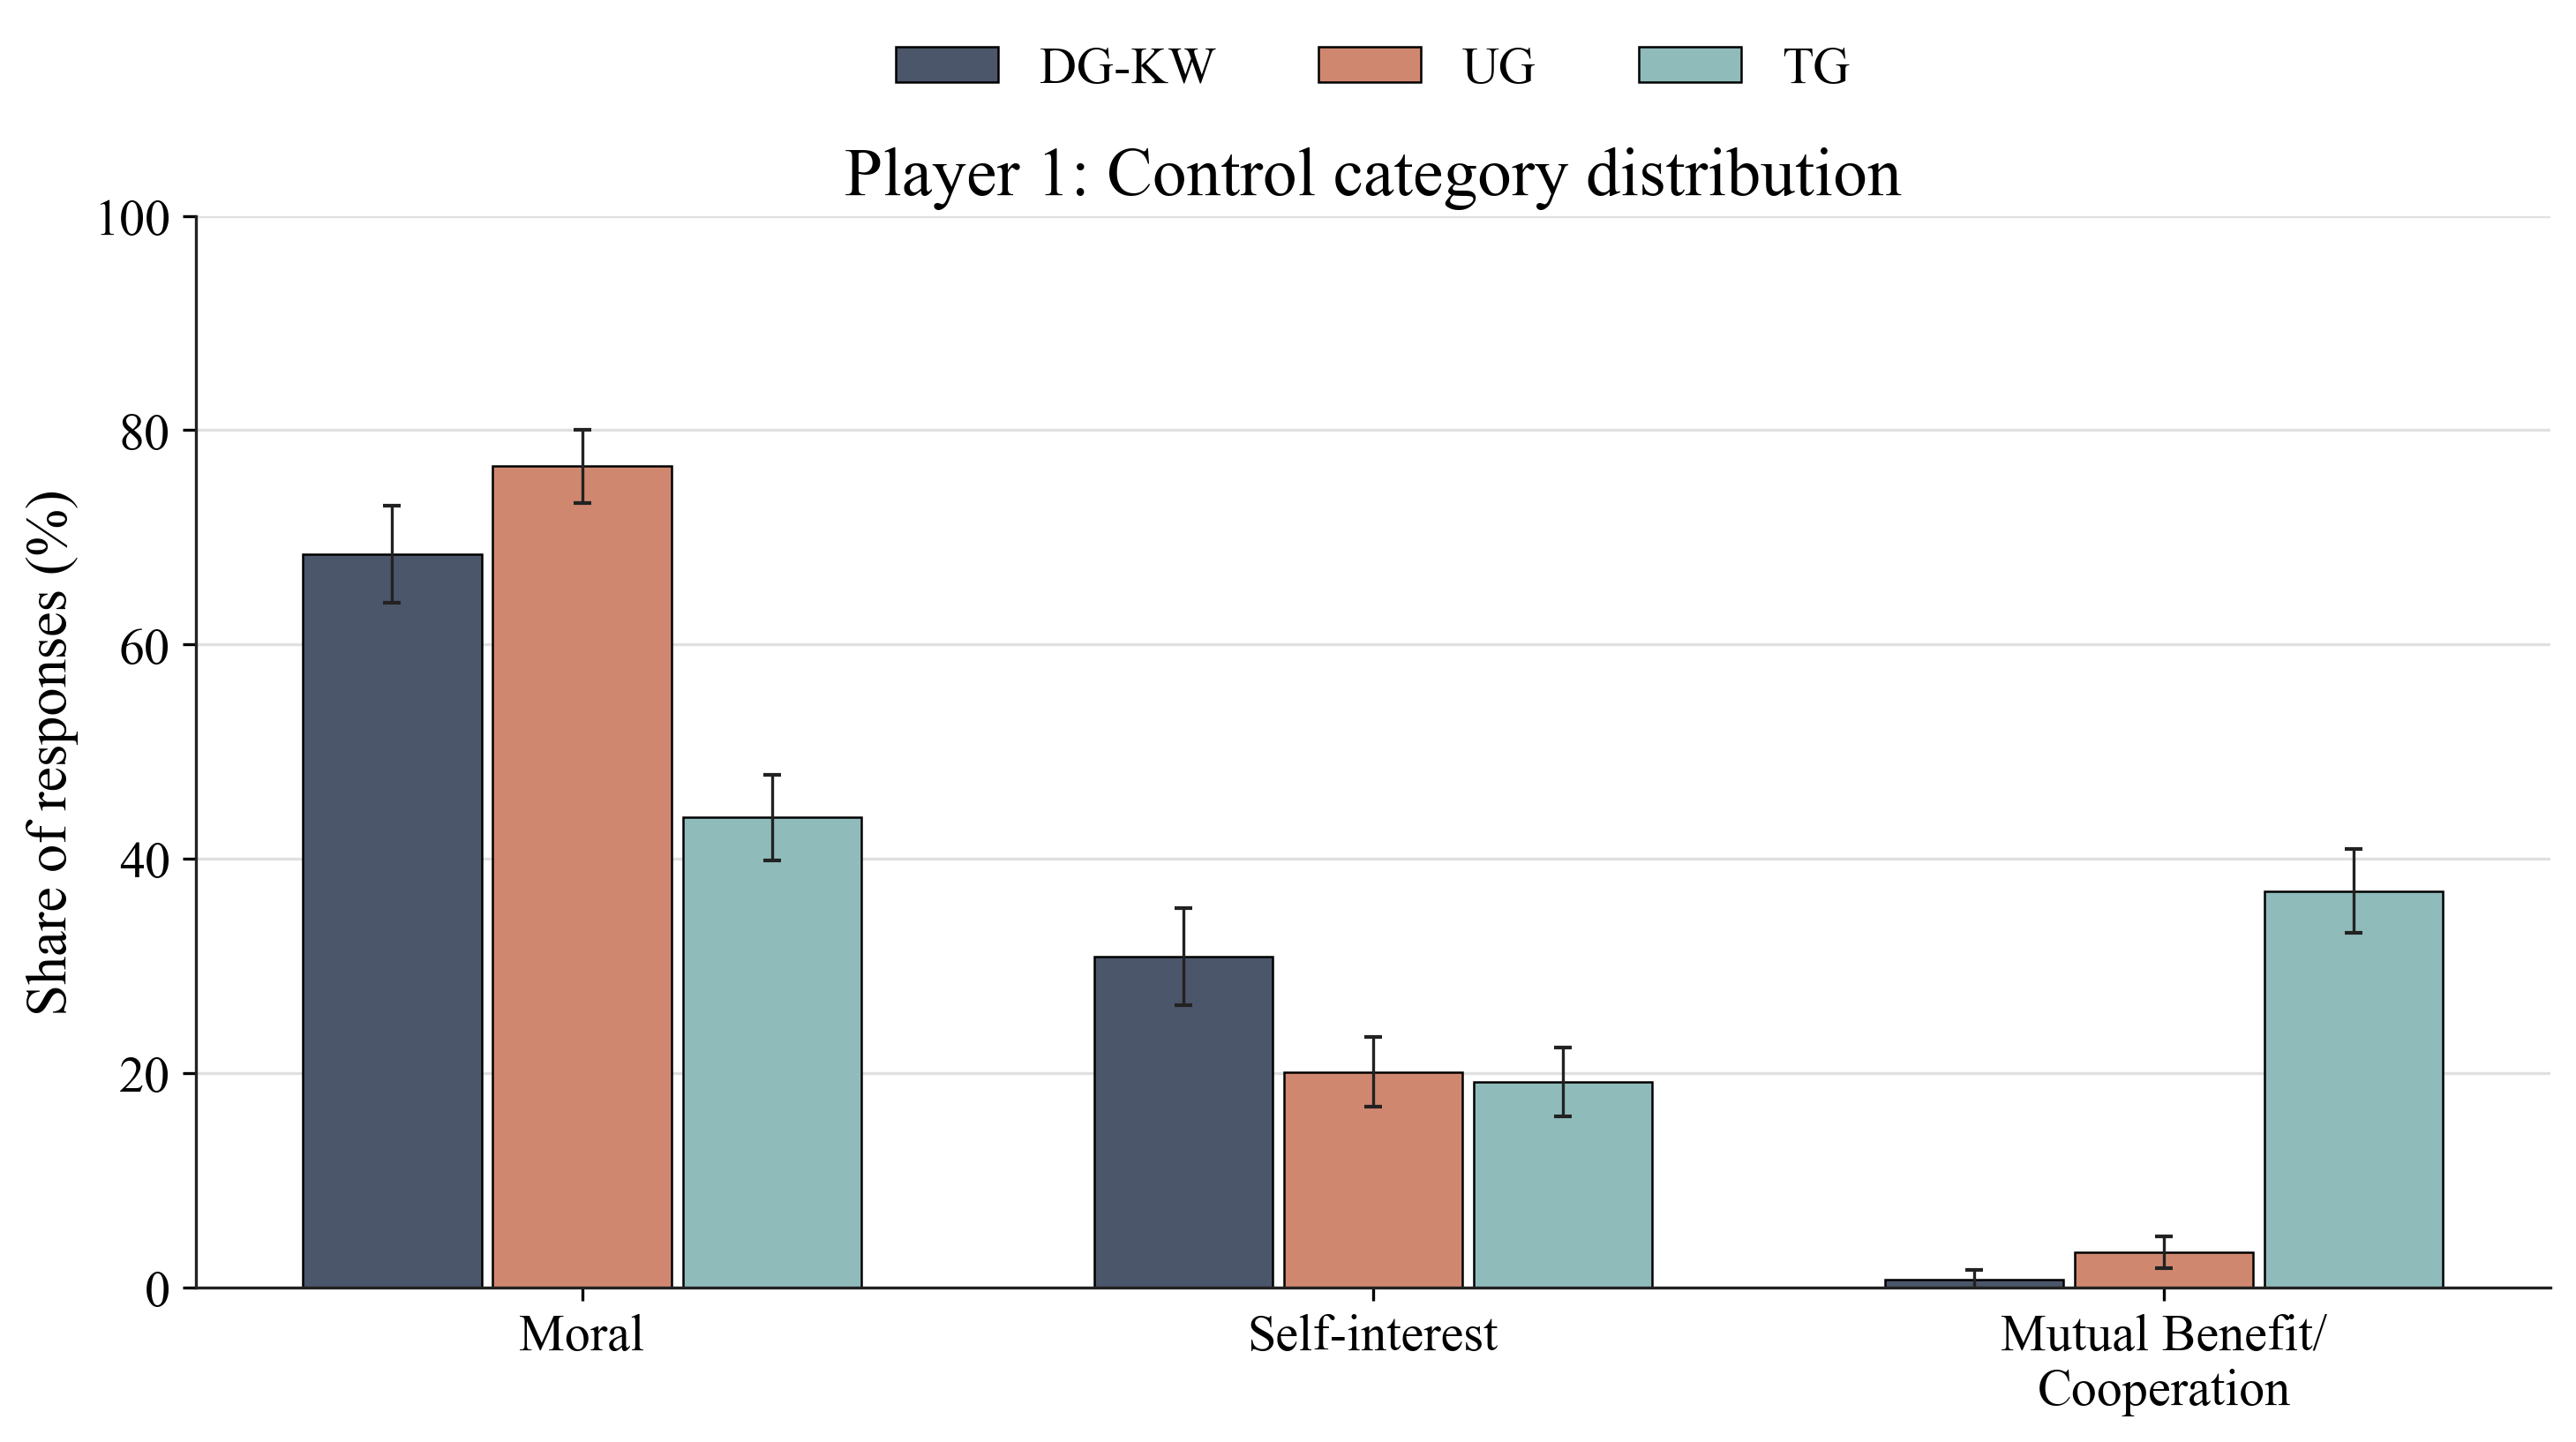
\includegraphics[width=0.82\textwidth]{player1_control_category_distribution_substantive_only.png}
\caption{Control-sample representation distributions for Player 1, excluding unclassified observations. Error bars show 95\% confidence intervals.}
\label{fig:control_cats}
\end{figure}

\paragraph{Social Proximity in Stated Reasons.} Stated reasons differ not only in the considerations they emphasize but also in whether and how they refer to the other player. The classification records whether a response refers to the counterpart and, when it does, the counterpart's social proximity; Table~\ref{tab:player1_sp_by_category} reports the resulting proximity classification within each stated reason category. Self-interested reasons are rarely paired with high social proximity (8.1\%), whereas high social proximity appears in 50.6\% of Moral reasons and 40.6\% of Mutual Benefit/Cooperation reasons. The social-proximity coding is also associated with behavior. In control, dictators whose response describes a close counterpart transfer 47.0\% of the budget, against 29.5\% for those whose response describes a distant counterpart or none; the same difference is 2.9 points in the ultimatum game and 10.1 points in the trust game. These patterns are consistent with participants who give different reasons also construing the counterpart differently.
% INSERTED 2026-07-16 (SP narrative per NG's 07-11 decision + AA's SP-as-bridge, SN approved): footnote promoted from the differ-across-games paragraph; tab:player1_sp_by_category moved here from app:player2; SP-action gaps (17.5/2.9/10.1pp) and market anonymity shares from the new SP block of output/tables/control_treatment_figure_stats.txt.

\begin{table}[!htbp]
\centering
\caption{\textbf{Player 1: Counterpart Proximity within Stated Reason Category}}
\label{tab:player1_sp_by_category}
\begin{tabular}{lccc}
\toprule
Counterpart proximity & Moral & Self-interest & Mutual Benefit/Cooperation \\
\midrule
Low social proximity & 49.4\% & 91.9\% & 59.4\% \\
High social proximity & 50.6\% & 8.1\% & 40.6\% \\
\bottomrule
\end{tabular}
\begin{flushleft}
\footnotesize Notes: Pooled across all games and treatments for Player 1. Columns report the distribution of counterpart proximity within each stated reason category and sum to 100\%.
\end{flushleft}
\end{table}


\paragraph{Representations and Actions.} Within each game, stated categories are systematically associated with actions, and these associations differ across strategic environments in the direction anticipated by the model. Figure~\ref{fig:control_outcomes} reports mean actions by category. Where a dictator faces no strategic response, the gap is large: moral dictators transfer 46.2\% of the budget and self-interested dictators 10.3\%. In the UG, the same category gap is much smaller: moral proposers offer 50.0\% and self-interested proposers 41.7\%, a pattern consistent with rejection risk constraining low offers. In the TG, cooperative senders send the most (63.5\%), moral senders 44.1\%, and self-interested senders 29.5\%. Thus, the same Self-interest category is associated with near-bottom transfers in the DG and near-fair offers in the UG.

\begin{figure}[!htbp]
\centering
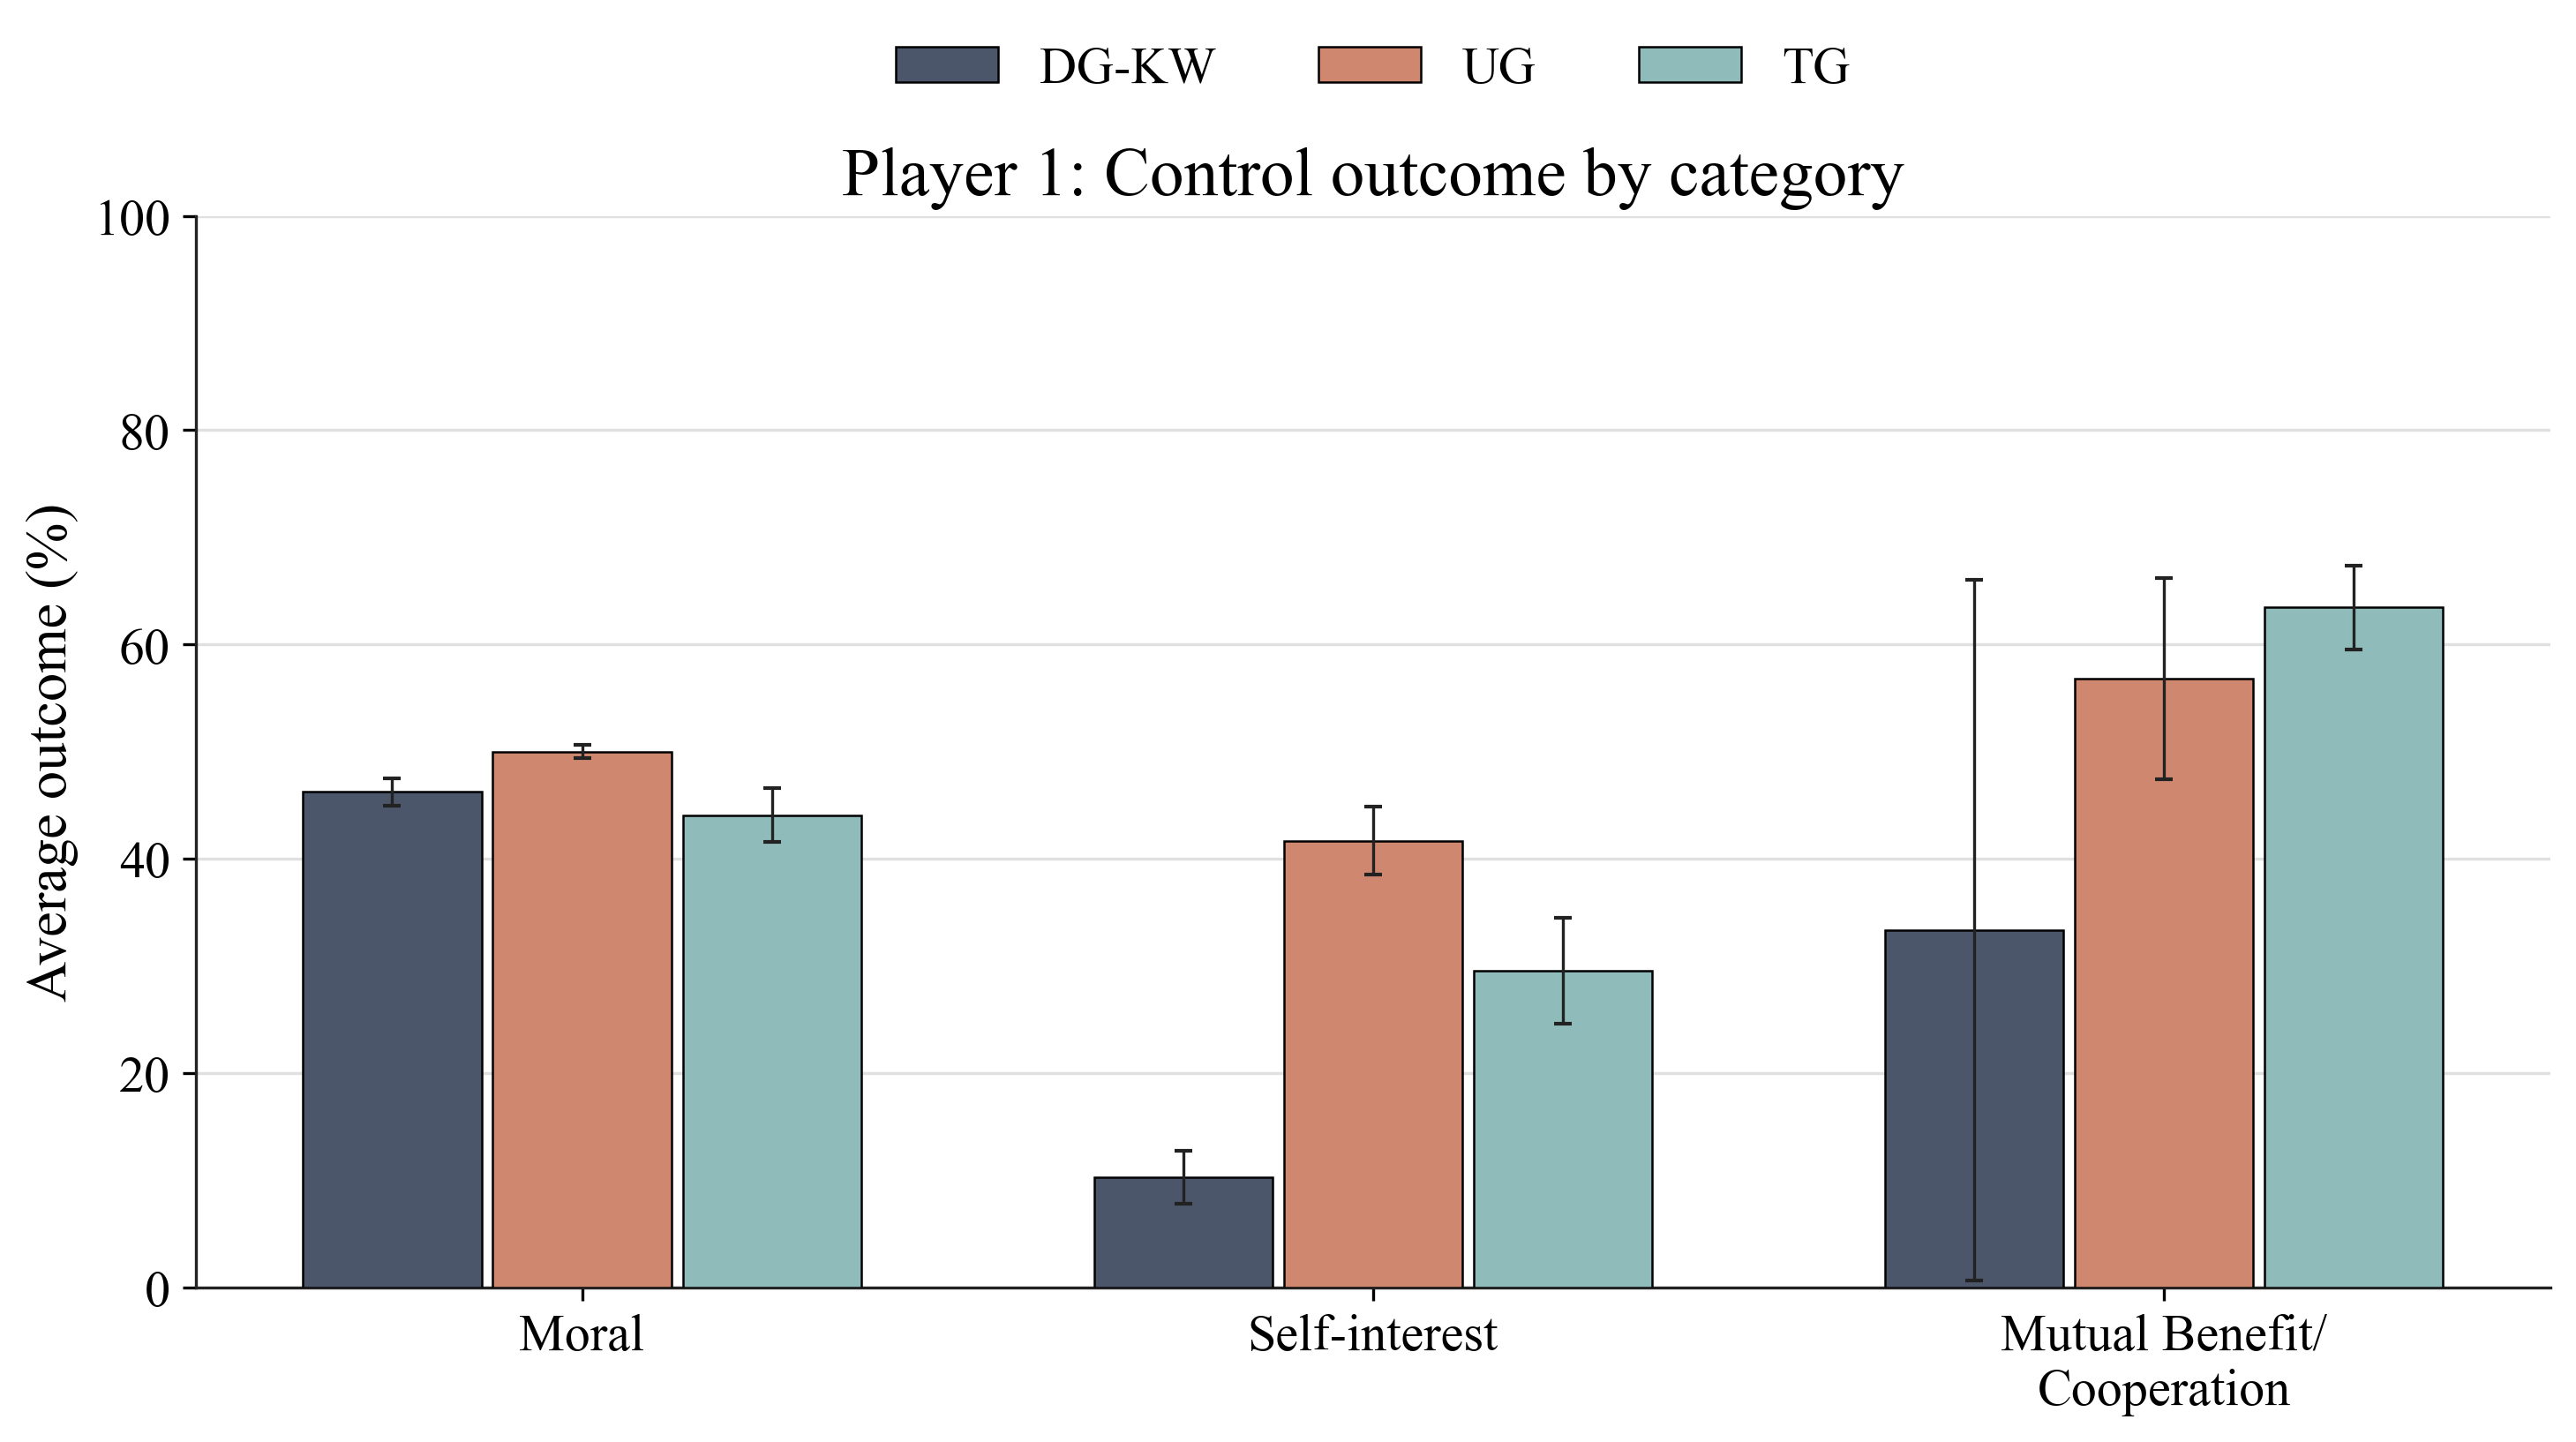
\includegraphics[width=0.82\textwidth]{player1_control_outcome_by_category_substantive_only.png}
\caption{Control-sample outcomes by category for Player 1. Outcomes are the share of the budget transferred (DG-KW), offered (UG), and sent (TG). The DG-KW Mutual Benefit/Cooperation cell contains very few observations (the category is 0.8\% of classified DG-KW responses) and should be read accordingly. Error bars show 95\% confidence intervals.}
\label{fig:control_outcomes}
\end{figure}

\paragraph{Representations and Beliefs.} The belief data reveal a sharp contrast between the UG and the TG. Figure~\ref{fig:control_beliefs} reports hypothetical beliefs at the one-third reference action. In the UG, beliefs about acceptance are essentially flat across categories (48.2--48.5\%): proposers in different categories report very similar acceptance expectations. These common beliefs may help explain why category differences in UG offers are much smaller than in dictator transfers. In the TG, by contrast, beliefs differ sharply across categories: self-interested senders expect back 22.0\% of the tripled amount, moral senders 31.5\%, and cooperative senders 35.7\%. Participants who describe the game as a cooperative venture also expect more cooperation from their counterpart, whereas those focused on own payoffs expect less. Together, these patterns are consistent with a common perceived acceptance standard in the UG and more category-specific expectations in the TG.

\begin{figure}[!htbp]
\centering
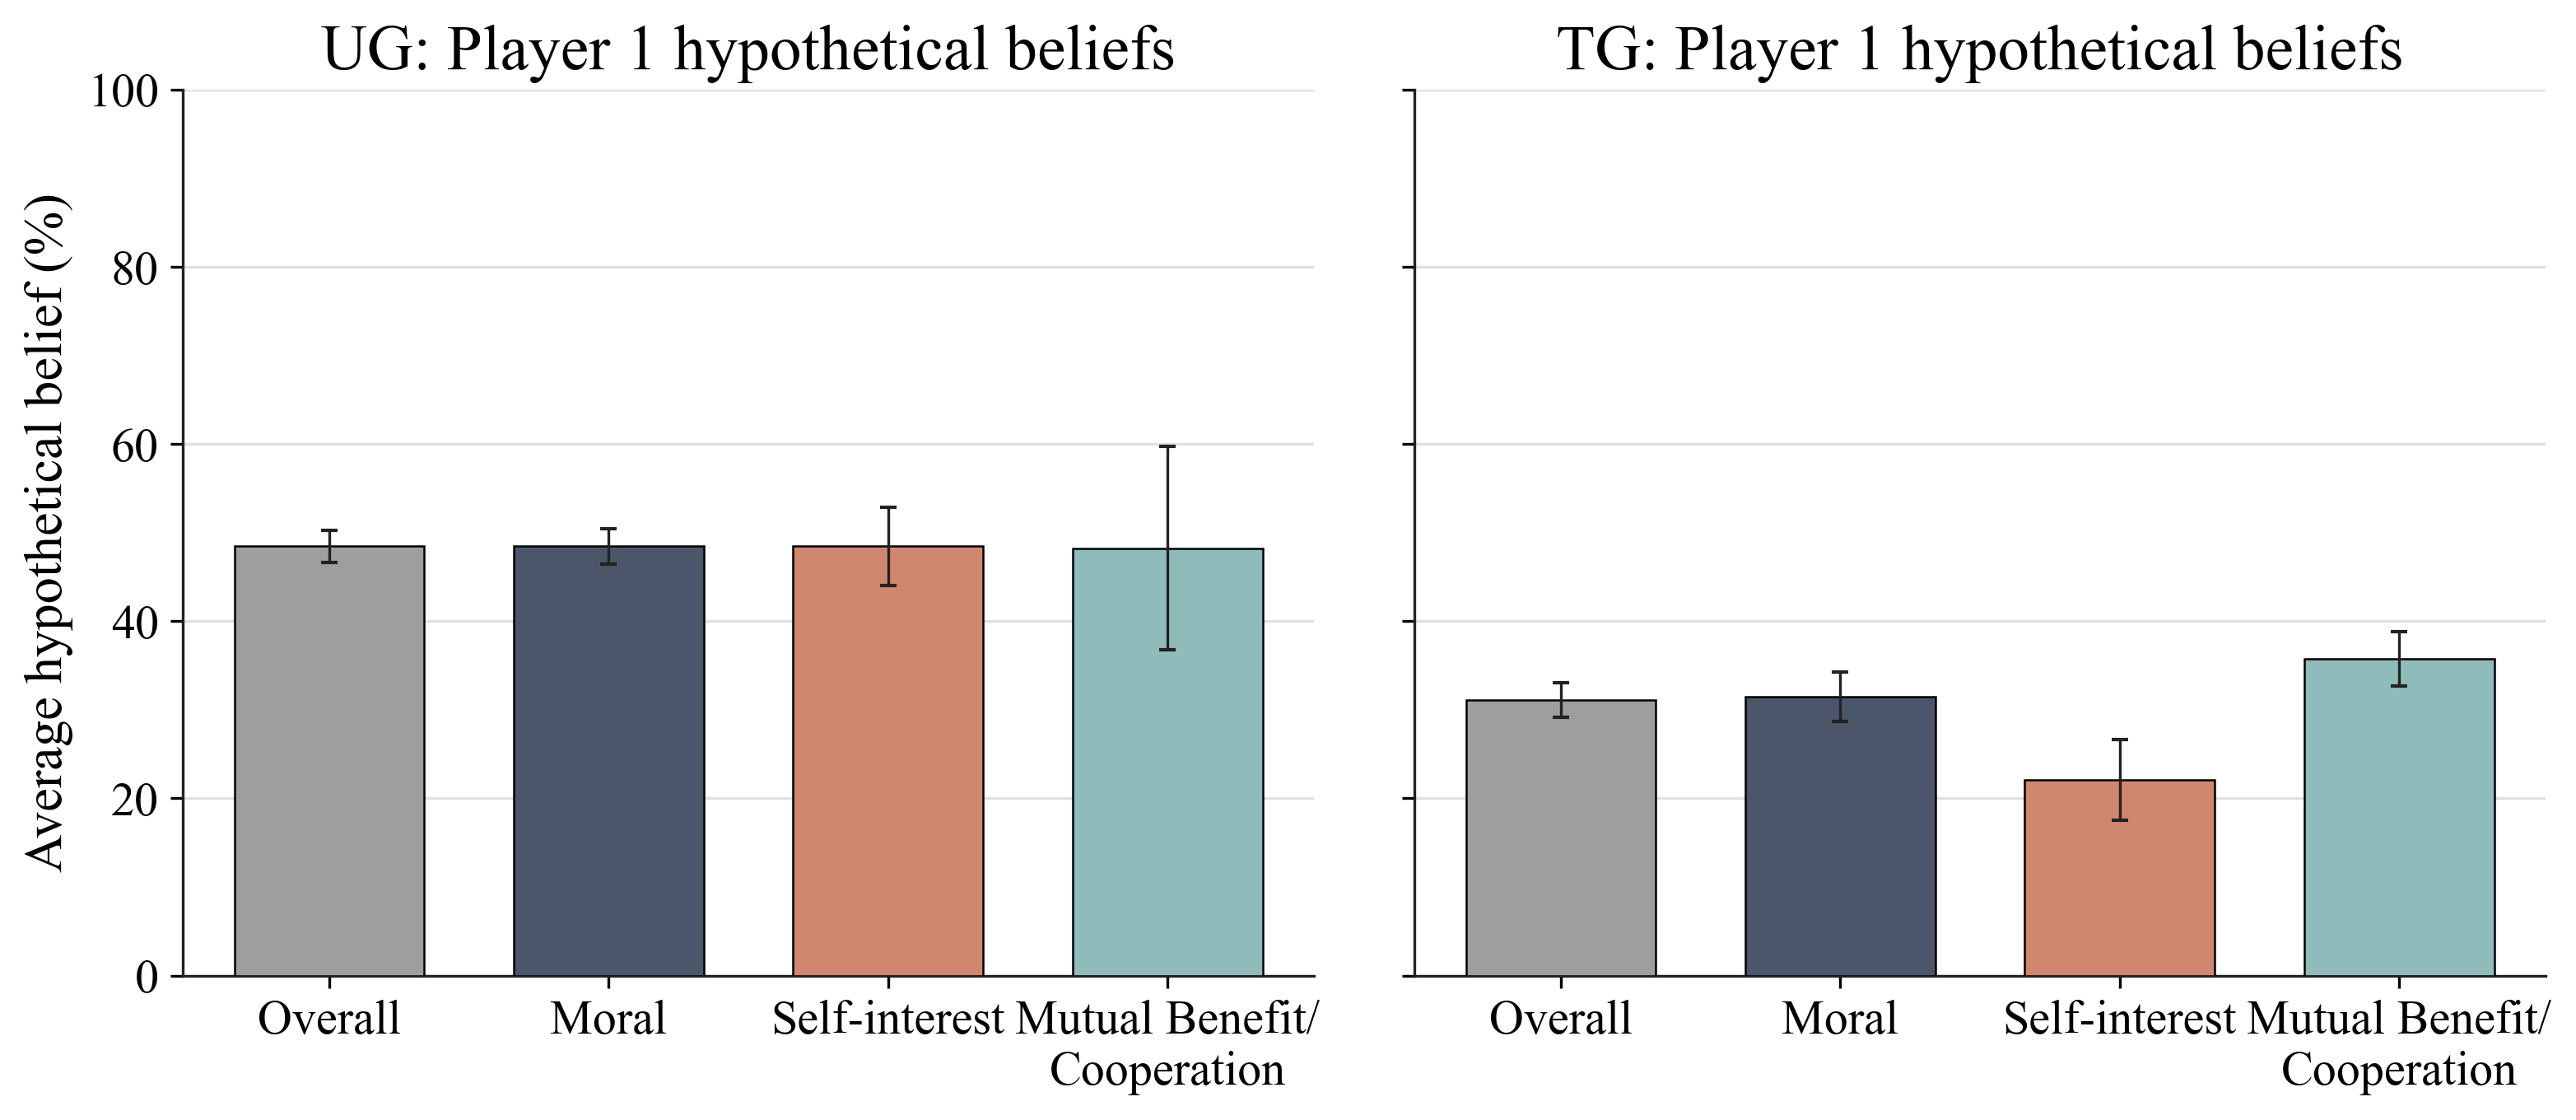
\includegraphics[width=0.92\textwidth]{player1_control_hp_beliefs_by_game.png}
\caption{Control-sample hypothetical beliefs for Player 1 at the common one-third reference action, split by UG and TG\@. Within each game, bars report the overall control-sample average and the category-specific means. Error bars show 95\% confidence intervals.}
\label{fig:control_beliefs}
\end{figure}

\paragraph{Actions and beliefs jointly.} Finally, the relationship between actions and beliefs also varies across categories. Figure~\ref{fig:belief_sensitivity} shows both patterns in the control data. In the UG, moral proposers' offers are essentially unrelated to their beliefs (slope $+0.01$), whereas self-interested proposers offer less when they believe a low offer is more likely to be accepted (slope $-0.11$). In the TG, sending rises with the believed return for every category, and the association is steepest for Self-interest ($+0.45$, against $+0.31$ for Moral). Pooling all four arms sharpens the estimates and rejects equality of slopes across categories in both games ($p=0.002$ in the UG and $p<0.001$ in the TG; Table~\ref{tab:belief_sensitivity} in Appendix~\ref{app:player2}). The pooled Mutual Benefit/Cooperation slope in the TG is the smallest of the three ($0.13$). Finally, the UG slopes are much smaller in magnitude than the TG slopes ($-0.09$ against $+0.47$ for Self-interest in the pooled specification), consistent with expected returns playing a more direct role in the trust game. These category-specific slopes underlie the pooled belief coefficients in the benchmark regressions of Section~\ref{sec:benchmark}.
% INSERTED 2026-07-16 (SN decision, AA-reproduction gate lifted): E1 figure + appendix table from 05 (restyled same day); every number above audited against output/tables/paper_v2_new_stats.txt this session (control slopes +0.010/-0.108/+0.451/+0.306; pooled -0.093/+0.465/+0.319/+0.128; UG pooled equality p=0.0015 -> table shows 0.002; TG pooled 0.0000).

\begin{figure}[!htbp]
\centering
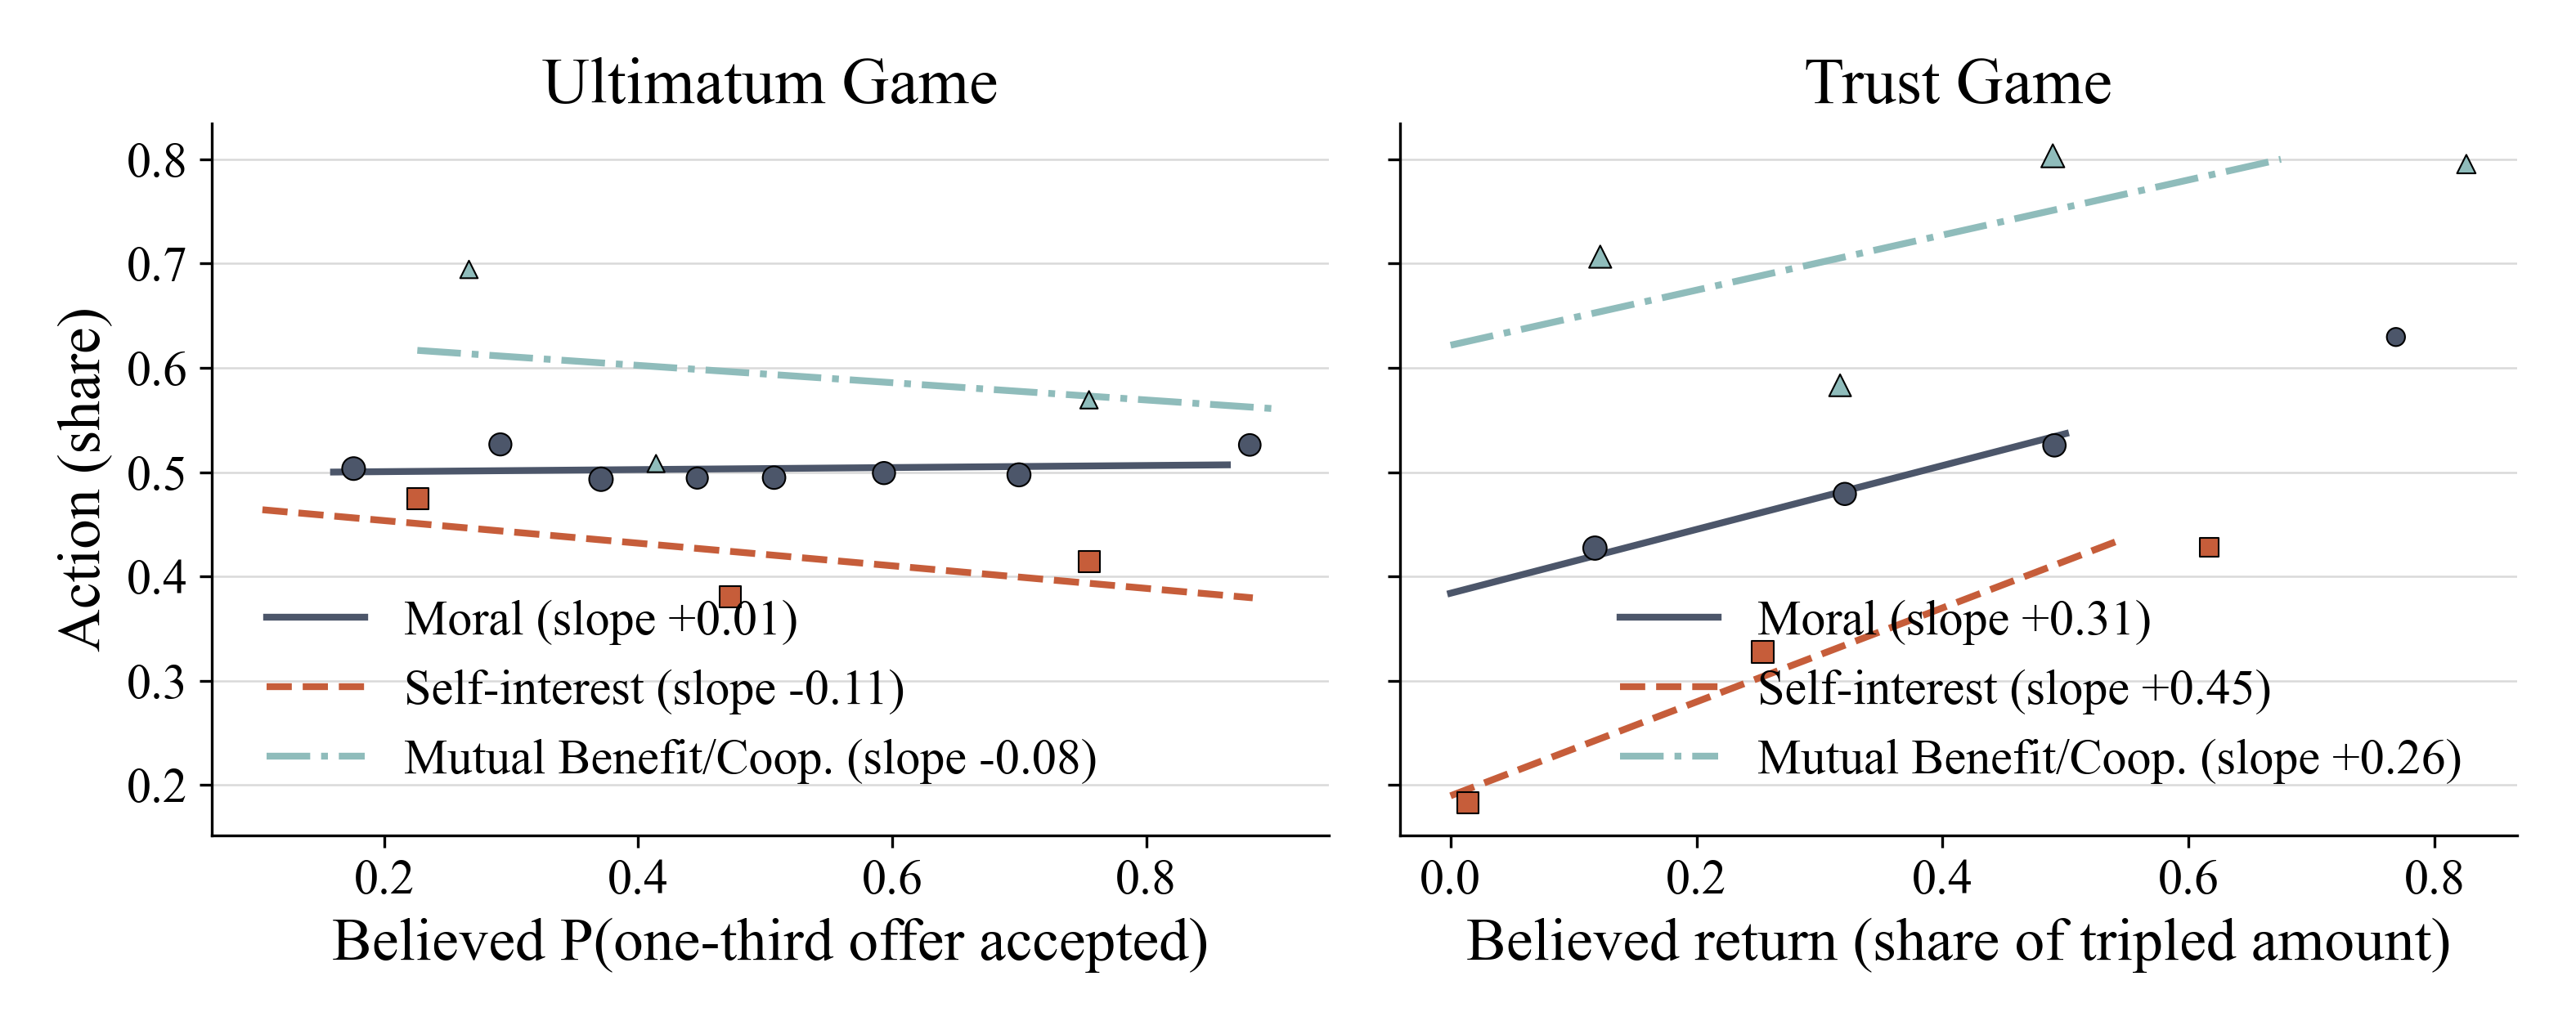
\includegraphics[width=0.9\textwidth]{player1_control_action_vs_belief_by_category.png}
\caption{Actions versus hypothetical beliefs by representation category, control sample. Points are quantile-binned means of the Player 1 action against the hypothetical belief at the one-third reference action (marker size increases with bin size); lines are category-specific OLS fits, with slopes in the legends. The UG Mutual Benefit/Cooperation cell is very small ($N=17$) and should be read accordingly. Slopes, standard errors, and pooled specifications are in Table~\ref{tab:belief_sensitivity}.}
\label{fig:belief_sensitivity}
\end{figure}

Appendix~\ref{app:player2} shows the same three facts for second movers: categories differ across games, predict hypothetical acceptance and returns (with \emph{Moral bad}---condemnation of the first mover---as the strongest predictor of rejection), and interact with the strategic environment as the model predicts.

These control results establish the empirical content of the representation measure: stated categories vary systematically with games, actions, and beliefs. The next subsection examines the similarity structure of the stories and games, yielding a prediction about where the story treatments should be most consequential. In the decomposition of Section~\ref{sec:determination}, a context manipulation moves mean behavior through a retrieval shift, whose size is gated by the similarity measured next and multiplied by the spread of category-typical actions documented above, widest where nothing disciplines the action.
% RESOLVED 2026-07-16 (was NOTE 2026-07-12): SP narrative implemented per NG's 07-11 decision (control SP above; market anonymity + generalized trust in Section 4.2); the one-sentence bridge to 3.3 is the sentence above.

\subsection{Treatments and Similarity}
\label{sec:similarity}

The retrieval model of Section~\ref{sec:determination} runs on similarity, and similarity is measurable. Ideally, we want the perceived similarity between our contexts---the two stories, the market and abstract descriptions---and both the games themselves and broad categories of experience (cooperation problems, conflict problems, moral problems), as well as receiver types (accepting or rejecting, returning or keeping). As a first pass, we measured the perceived \emph{structural} similarity between the two stories and the four games using large language models as raters; a human-subjects survey replicating and extending the module is in progress.
% TODO: field the human similarity survey (design in similarity_survey_design.md) and extend the LLM module to category-level similarity (contexts x {cooperation, conflict, moral} and receiver types), per NG's ``ideal thing to do'' in the skeleton.

Three frontier models each rated, in three separate conversations with independently permuted neutral labels (games presented as A--D, stories as Story 1/Story 2, to rule out position effects and priors about the experimental literature), the similarity of each story to each game on a 0--100 scale, decomposed the games' structure along five dimensions, and reported, for each game, which story it called to mind (a 100-point split). This yields 72 similarity ratings across nine conversations; the findings below hold in every model and every permutation, with small ranges across label permutations.\footnote{Prompts, the nine transcripts, and the recording workbook are in the replication package.}

\begin{table}[!htbp]
\centering
\footnotesize
\renewcommand{\arraystretch}{1.15}
\caption{\textbf{Perceived Similarity of Stories to Games, LLM Raters}}
\label{tab:llm_similarity}
\begin{tabular}{l ccc c}
\toprule
& \multicolumn{3}{c}{Structural similarity (0--100)} & Retrieval split \\
\cmidrule(lr){2-4}\cmidrule(lr){5-5}
Game & Bonus & Aid & Mean & Bonus / Aid \\
\midrule
DG-KW & 94.6 & 94.7 & 94.6 & 41 / 59 \\
DG-LT & 51.8 & 50.7 & 51.2 & 54 / 46 \\
UG    & 30.1 & 29.8 & 29.9 & 60 / 40 \\
TG    & 15.0 & 13.9 & 14.4 & 72 / 28 \\
\bottomrule
\end{tabular}
\begin{flushleft}
\footnotesize Notes: Means over nine conversations (three models $\times$ three label permutations). Structural similarity: 0--100 rating of each story--game pair. Retrieval split: 100 points divided between the two stories according to which the game calls to mind as a similar experience.
\end{flushleft}
\end{table}

Table~\ref{tab:llm_similarity} reports three findings. First, the games differ sharply in their structural distance from the stories, in a fixed order: DG-KW ($94.6$) $>$ DG-LT ($51.2$) $>$ UG ($29.9$) $>$ TG ($14.4$). Every model identifies the budget structure---expandable versus fixed---as the dimension that isolates the trust game from the other three: the gains from cooperation are what make the TG a structurally different situation. Second, \emph{Bonus and Aid are structurally indistinguishable}: their similarity ratings differ by at most 1.1 points for any game. Whatever behavioral differences the two stories produce cannot run through a differently perceived game structure; the stories are the same situation seen from two contexts, which is exactly what the story lever of Section~\ref{sec:determination} requires---it moves $F_c$ while the description stays put---and what a game-specific-norms account cannot use. Third, the \emph{retrieval} direction tells a different story from structural similarity: asked which story each game calls to mind, the models assign Bonus a share that rises monotonically with strategic richness---41\% in DG-KW, 54\% in DG-LT, 60\% in the UG, 72\% in the TG---even though structural similarity is flat across the two stories. Surface and contextual cues in the Bonus story (joint production, an ongoing work relationship) increasingly dominate retrieval as the game acquires strategic structure, precisely the wedge between similarity of structure and similarity of context on which the retrieval model runs.

The structural-distance ordering yields a discipline on the story treatments that we use in Section~\ref{sec:aid_bonus}: if similarity gates retrieval, the boost that a story gives to its category should matter most where the story is structurally close to the game and vanish where it is remote---largest in the dictator games, smaller in the ultimatum game, absent in the trust game. With only four games this is a coarse check, but it is one the data can fail.

\section{Treatment Effects on Representations and Sender Behavior}
\label{sec:treatment}

Having established how representations organize behavior when context is held fixed, we turn to the randomized context manipulations. For each comparison and game, we report treatment effects on three objects: representation shares, actions, and hypothetical beliefs.\footnote{The figures in this section are drawn on the classified sample---the category panels require it, and each figure uses one sample throughout---while the effect sizes quoted in the text and in the tables use all responses (the residual unclassified category is 1--3.5\% of responses). Cell by cell, the two conventions differ by less than one percentage point; both sets are logged in the replication package.} Signs implied by the model (via the category-to-weights mapping of Section~\ref{sec:mapping}, applied to the measured representation shifts) are marked in the figures when the outcome effect is statistically distinguishable from zero and the model's prediction is unambiguous. The two comparisons manipulate different aspects of context. Aid versus Bonus varies the narrative presented before the abstract game, whereas Market versus Control changes the description of the interaction itself. We interpret these treatments through the two levers of Section~\ref{sec:determination}: the stories as shifting retrieval frequency ($F_c$), and the market frame as changing the context of the description ($\boldsymbol{\kappa}_d$).

\subsection{Stories: Aid vs Bonus}
\label{sec:aid_bonus}

Reading a story about charitable aid, relative to a story about a workplace bonus, makes representations \emph{less} moral and \emph{more} self-interested in the two sharing games---and behavior follows (Figure~\ref{fig:te_aid_bonus}). Moral falls by 11.7 percentage points in the DG-KW and 9.7 in the UG, and Self-interest rises by 11.5 and 10.4 points; the TG is unaffected on every margin. Dictator transfers fall by 5.6 percentage points of the budget and UG offers by 2.4 points, while TG sends do not move (+0.5, n.s.). Beliefs do not move either (+1.2 points in the UG, $-$1.6 in the TG, both n.s.), consistent with the representation shift operating through first movers' own weights rather than through their forecasts.

A charitable context does not prime generosity: if anything, a story about need and scarcity licenses self-interest relative to a story about workplace achievement. Context operates not by cueing a behavior (``be generous'') but by changing what the situation is \emph{about}---a pattern consistent with stories of hardship directing attention to one's own material stakes. The stories differ in more than setting---the aid story voices the temptation to keep, the bonus story the case for sharing (Appendix~\ref{app:instructions})---so we read the comparison as story content shifting which considerations the game evokes, rather than as isolating hardship per se; the substantive point, that a charitable context fails to trigger generosity, stands either way.

\begin{figure}[!htbp]
\centering
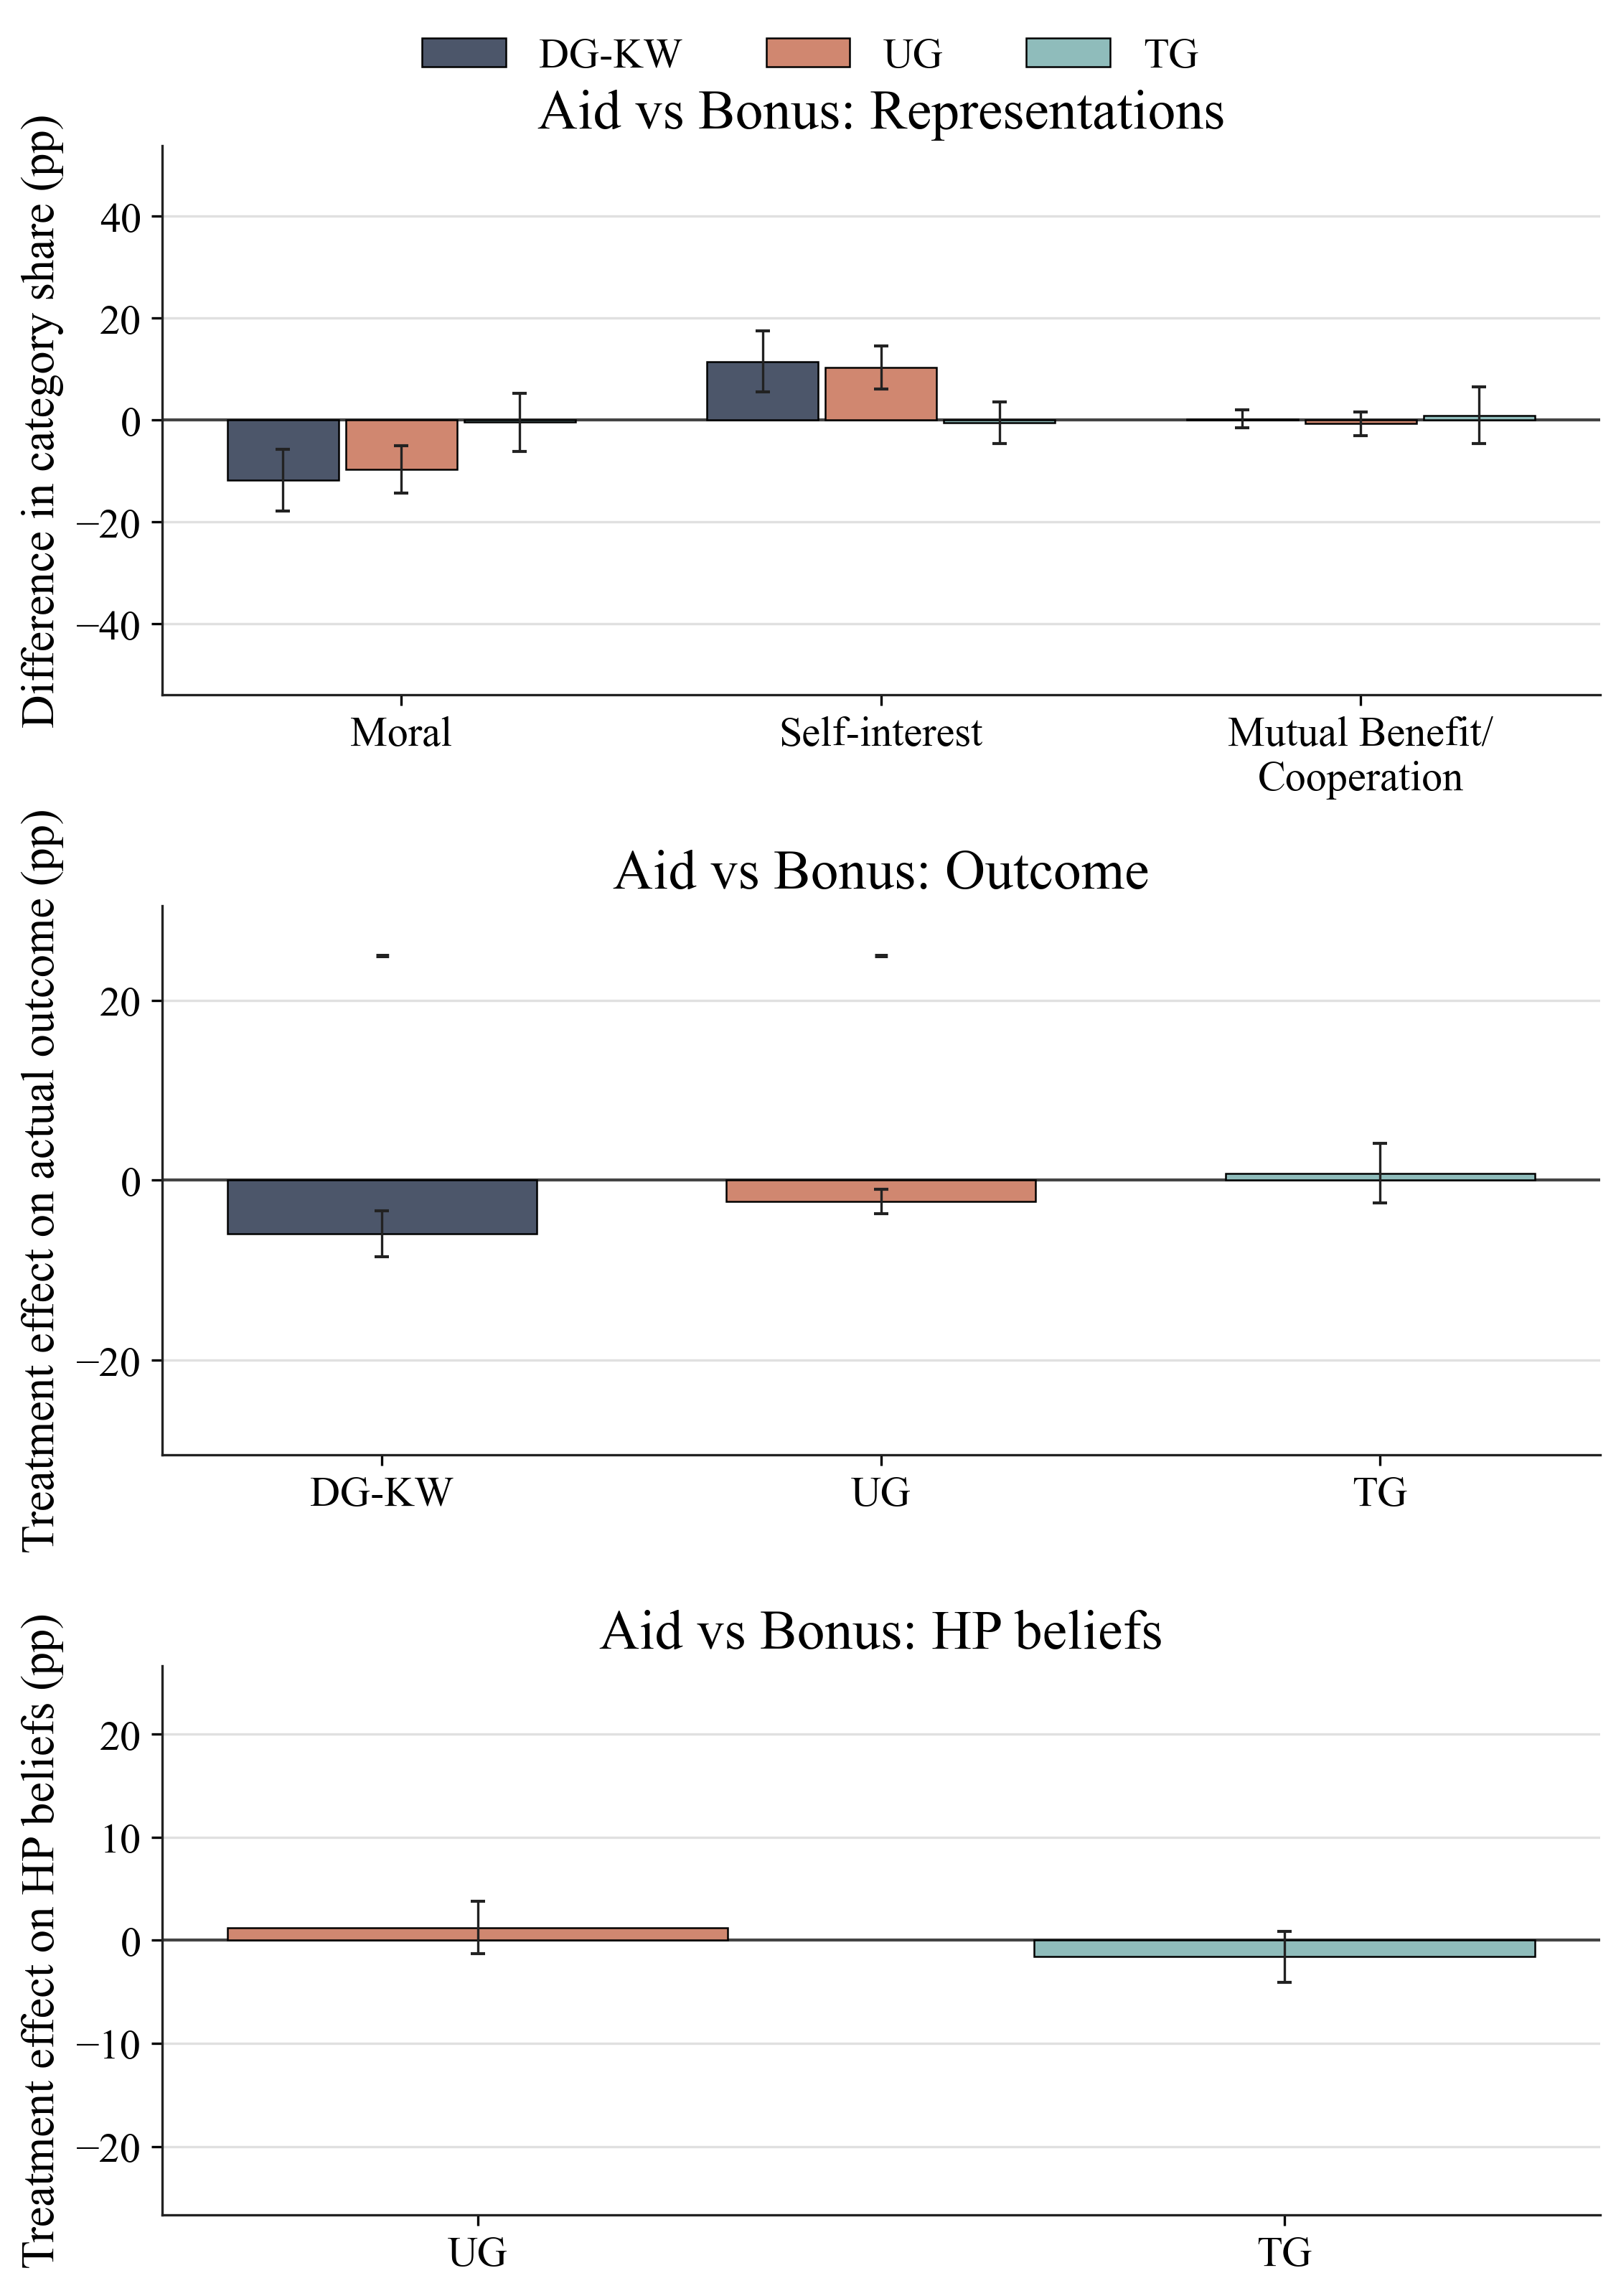
\includegraphics[width=0.78\textwidth]{paper_section4_player1_aid_vs_bonus.png}
\caption{Aid vs Bonus treatment effects for Player 1. The first panel shows treatment-induced shifts in category shares, the second panel shows treatment effects on actual outcomes with model-predicted direction markers, and the third panel shows treatment effects on hypothetical beliefs at the common one-third reference action. A plus or minus sign appears only when the corresponding outcome effect is statistically distinguishable from zero and the model prediction is unambiguous. Error bars show 95\% confidence intervals.}
\label{fig:te_aid_bonus}
\end{figure}

Figure~\ref{fig:te_aid_bonus} displays two patterns consistent with the model's interpretation of the story treatment. First, reported categories and actions move while hypothetical beliefs remain close to zero, consistent with the treatment shifting the considerations participants bring to the game rather than their forecasts of the other player. Second, the effects fade with the structural distance between the stories and the game measured in Section~\ref{sec:similarity} (Table~\ref{tab:llm_similarity}).

Table~\ref{tab:similarity_gradient} places these patterns alongside the structural-similarity ratings, adding DG-LT, the give-or-take dictator game of Figure~\ref{fig:intro_kw_lt} (its story arms appear here and in the dispersion accounting of Section~\ref{sec:heterogeneity}). Story effects on actions decline monotonically as measured similarity falls: $-5.6$, $-4.7$, $-2.4$, and $+0.5$ (n.s.) percentage points as similarity falls from 94.6 to 51.2 to 29.9 to 14.4. The effect on stated representations shows a similar pattern: the Moral share falls by 9.7 to 14.5 points in the three more structurally similar games and by a negligible 0.4 points in the TG. This ordering is consistent with the prediction that story-induced retrieval shifts matter less when the story and game are structurally remote. With only four games and LLM-based similarity ratings, however, it is an ordinal, exploratory consistency check rather than a separately identified estimate. The negligible TG effects coincide with both a negligible shift in Moral reasoning and the lowest measured similarity to the stories; they do not by themselves establish why trust-game sending is unchanged.
% INSERTED 2026-07-16 (SN decision, AA-reproduction gate lifted): E5 table from 05; numbers audited against output/tables/paper_v2_new_stats.txt this session (action effects -5.6/-4.7/-2.4/+0.5; Moral-share -11.7/-14.5/-9.7/-0.4; similarity 94.6/51.2/29.9/14.4). DG-LT Aid-Bonus was previously unreported anywhere.

\begin{table}[!htbp]
\centering
\small
\renewcommand{\arraystretch}{1.15}
\caption{\textbf{Story Effects Track the Structural Similarity of Stories to Games}}
\label{tab:similarity_gradient}
\begin{tabular}{l cc rr}
\toprule
 & Structural & Bonus retrieval & \multicolumn{2}{c}{Aid $-$ Bonus effect (pp)} \\
\cmidrule(lr){4-5}
Game & similarity (0--100) & share (\%) & Action & Moral share \\
\midrule
DG-KW & 94.6 & 41 & $-5.6$ & $-11.7$ \\
DG-LT & 51.2 & 54 & $-4.7$ & $-14.5$ \\
UG & 29.9 & 60 & $-2.4$ & $-9.7$ \\
TG & 14.4 & 72 & $+0.5$ & $-0.4$ \\
\bottomrule
\end{tabular}
\begin{flushleft}
\footnotesize Notes: Structural similarity and retrieval shares are means over the nine LLM conversations (Section on Treatments and Similarity); action and Moral-share effects are Aid $-$ Bonus differences (Player 1; Moral share among classified responses). The treatment-effect figures of Section 4 use DG-KW, UG, TG\@; the DG-LT story conditions enter this table and the dispersion accounting of Section 5.
\end{flushleft}
\end{table}


\subsection{Interaction Frame: Market vs Control}
\label{sec:market_control}

Framing the identical interaction as a market transaction does not simply make people selfish: it replaces the ethics of sharing with a mixture of own-payoff reasoning and joint-gains reasoning (Figure~\ref{fig:te_market_control}). Moral representations fall in every game---by 27.4 percentage points in the DG-KW, 42.7 in the UG, and 23.8 in the TG---while \emph{both} Self-interest (+10.5, +16.8, +5.5) and Mutual Benefit/Cooperation (+16.9, +25.9, +18.3) rise.

Behavior tracks the attention weights game by game. Where the pie is fixed and efficiency attention is idle, transfers fall exactly as the moral-to-self-interest shift predicts: dictator giving falls by 10.9 percentage points and UG offers by 21.9 points (95\% CI $[-24.2, -19.6]$). In the TG, where efficiency attention is the engine of sending, sends \emph{rise} by 14.5 points (95\% CI $[11.3, 17.7]$), in line with the rise of cooperative representations. Beliefs move in the same direction as the cooperative shift: proposers become markedly more optimistic that a one-third offer would be accepted (+17.2 points) and senders more optimistic about repayment (+10.3 points). Second movers show the mirror image: the market frame shifts their representations the same way, yet their hypothetical acceptance and returns \emph{rise} by about 10 points (Section~\ref{sec:ge}).

\begin{figure}[!htbp]
\centering
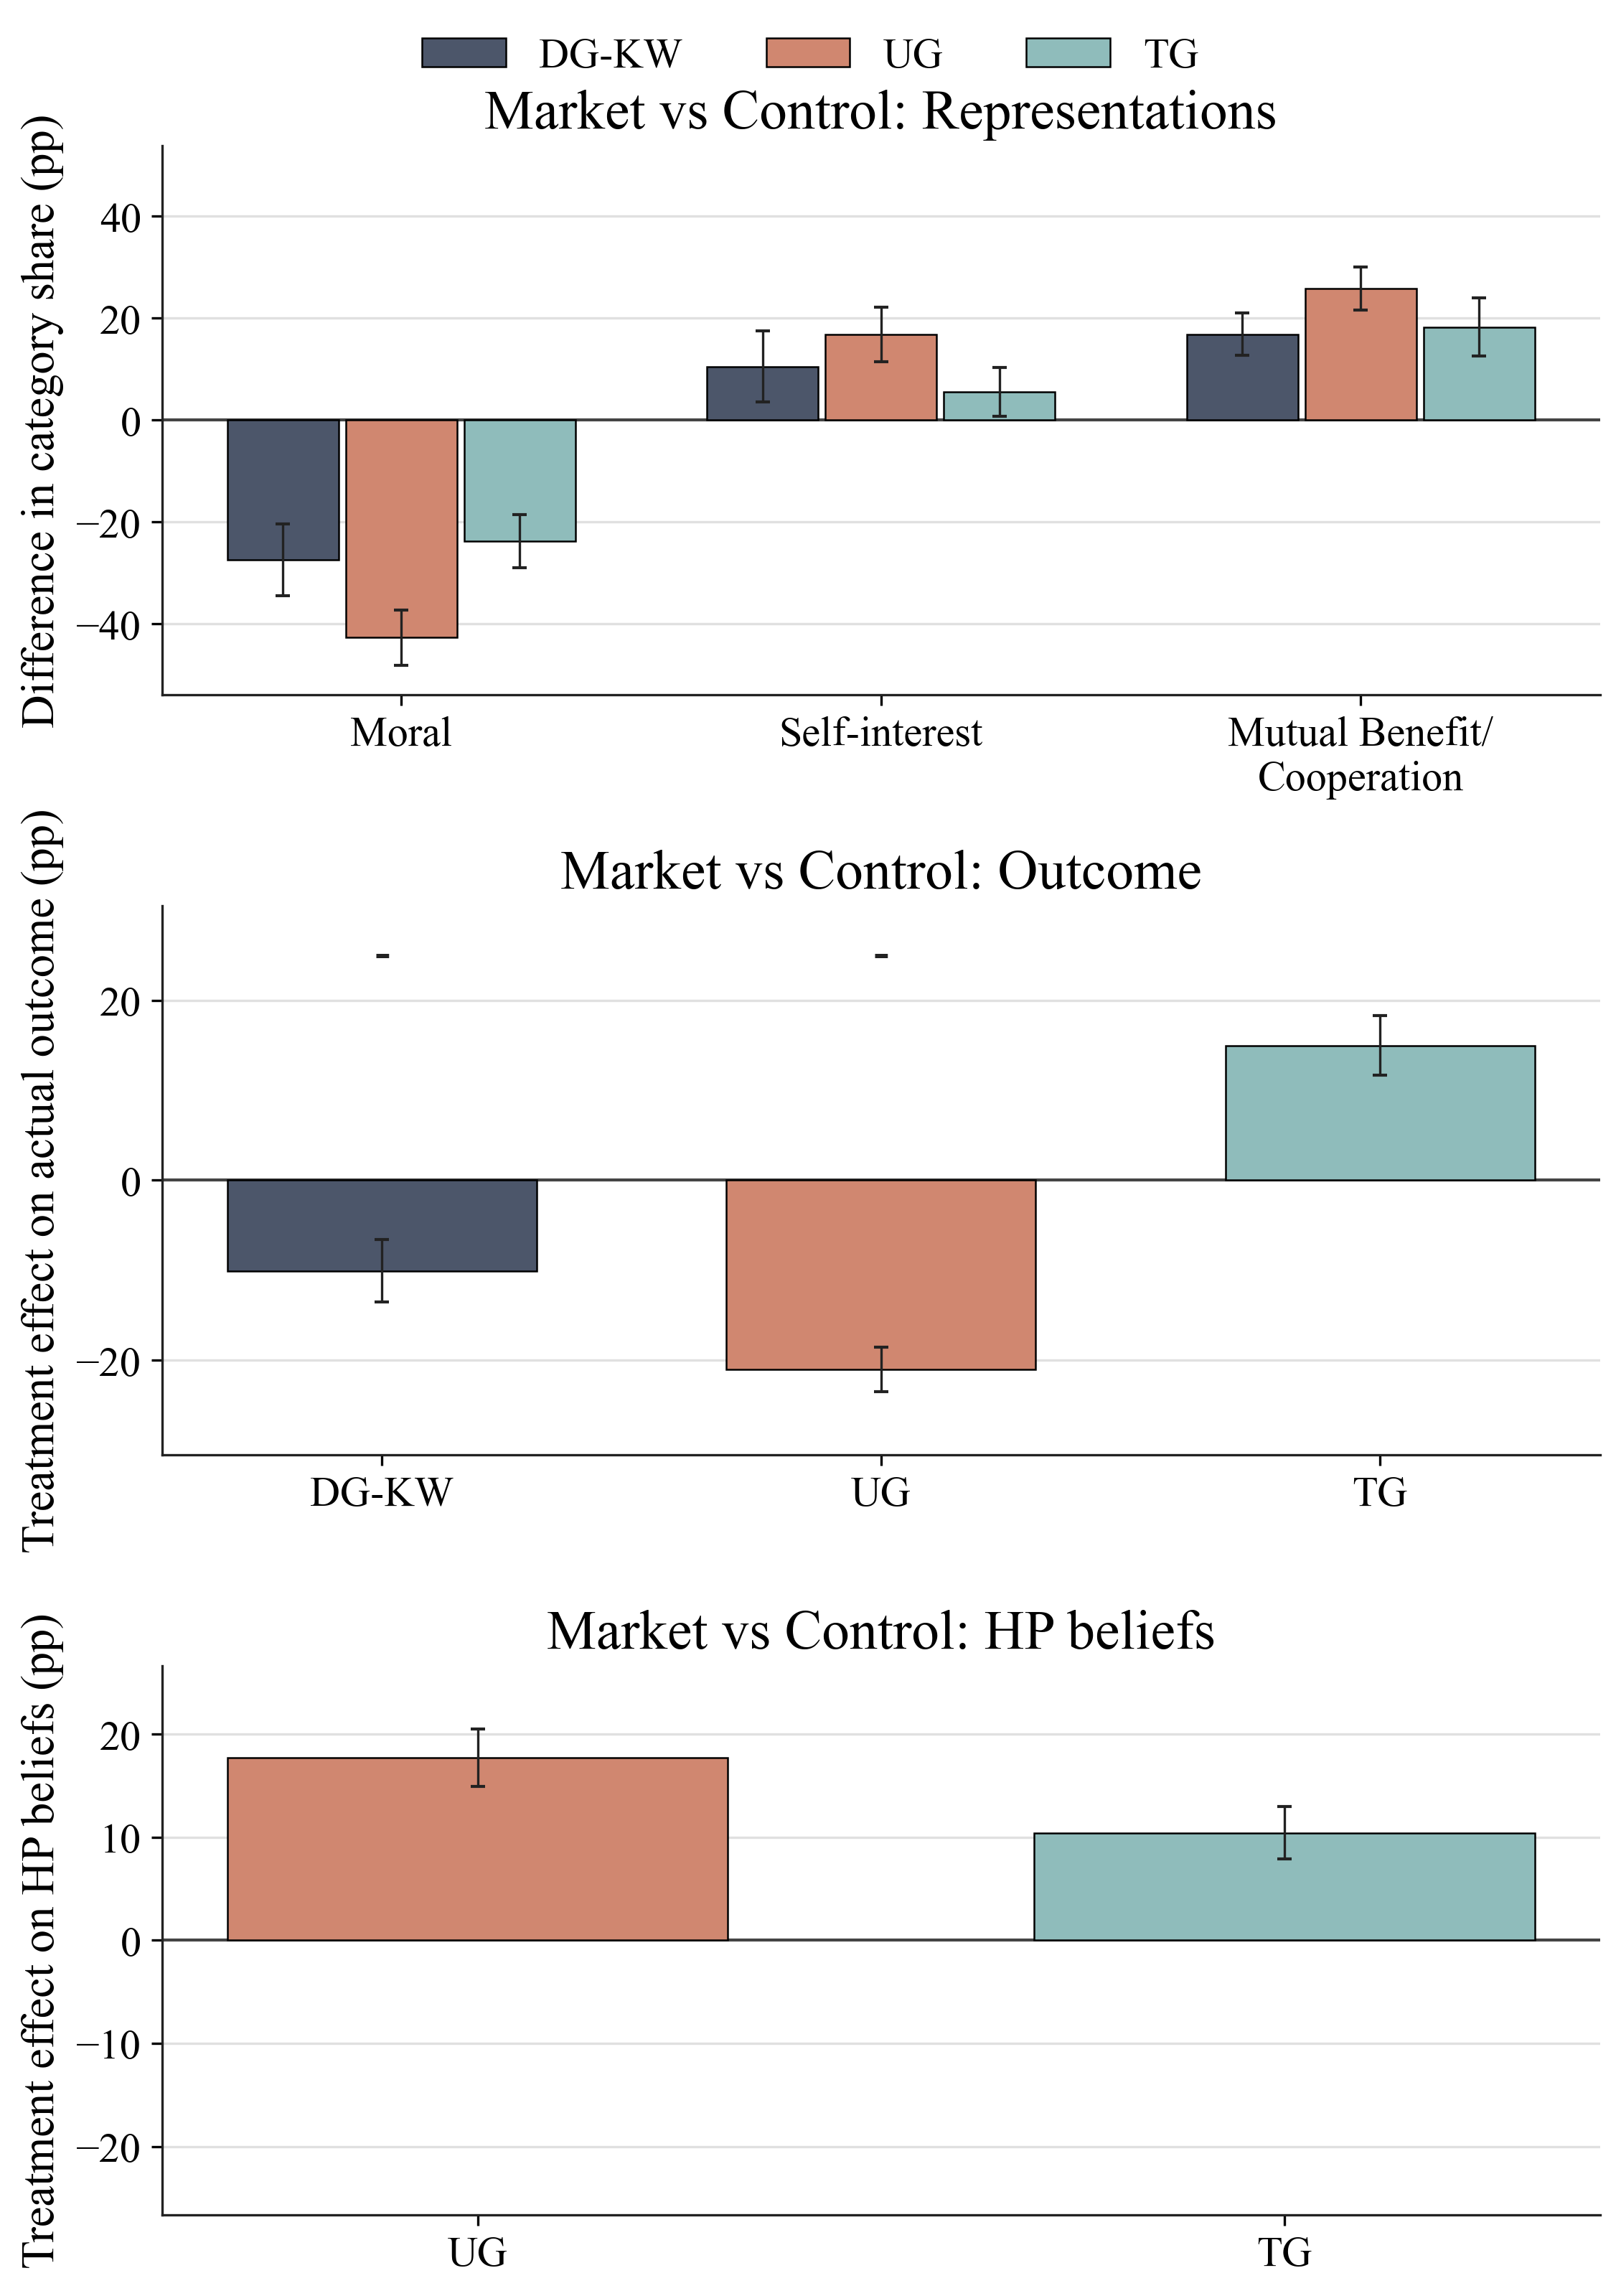
\includegraphics[width=0.78\textwidth]{paper_section4_player1_market_vs_control.png}
\caption{Market vs Control treatment effects for Player 1. Panels as in Figure~\ref{fig:te_aid_bonus}. Error bars show 95\% confidence intervals.}
\label{fig:te_market_control}
\end{figure}

Treatment effects on means understate what the frame does. Figure~\ref{fig:market_distributions} plots the full distributions of Player 1 actions. The market frame does not slide a distribution of mostly-fair choices toward selfishness; it dissolves the equal-split anchor. In the UG, the share of proposers offering exactly half collapses from 76.5\% to 18.3\% while zero offers rise from 1.0\% to 32.0\%; in the DG-KW, the even-split spike falls from 51.4\% to 14.0\% and zero transfers rise from 18.9\% to 37.2\%. In the TG, mass moves the other way, toward the maximum: full sends rise from 16.0\% to 27.0\%. A shift in a single generosity or selfishness parameter would translate these distributions; what the data show is mass moving between qualitatively different actions---the norm anchor, zero, the maximum---which is what a change in the mixture of representations, each with its own anchor, produces. Section~\ref{sec:heterogeneity} returns to this in variance terms.
% INSERTED 2026-07-16 (SN decision, AA-reproduction gate lifted): E2 figure from 05 (restyled same day); spike shares logged by 05 this session (DG-KW 0.514->0.140 at $6, 0.189->0.372 at $0; UG 0.765->0.183, 0.010->0.320; TG 0.160->0.270 at $6); KS D=0.320/0.580/0.283, p=1.2e-18/1.0e-93/1.3e-21 -> "all p<1e-17" (NOT 1e-18: the DG-KW p exceeds 1e-18).

\begin{figure}[!htbp]
\centering
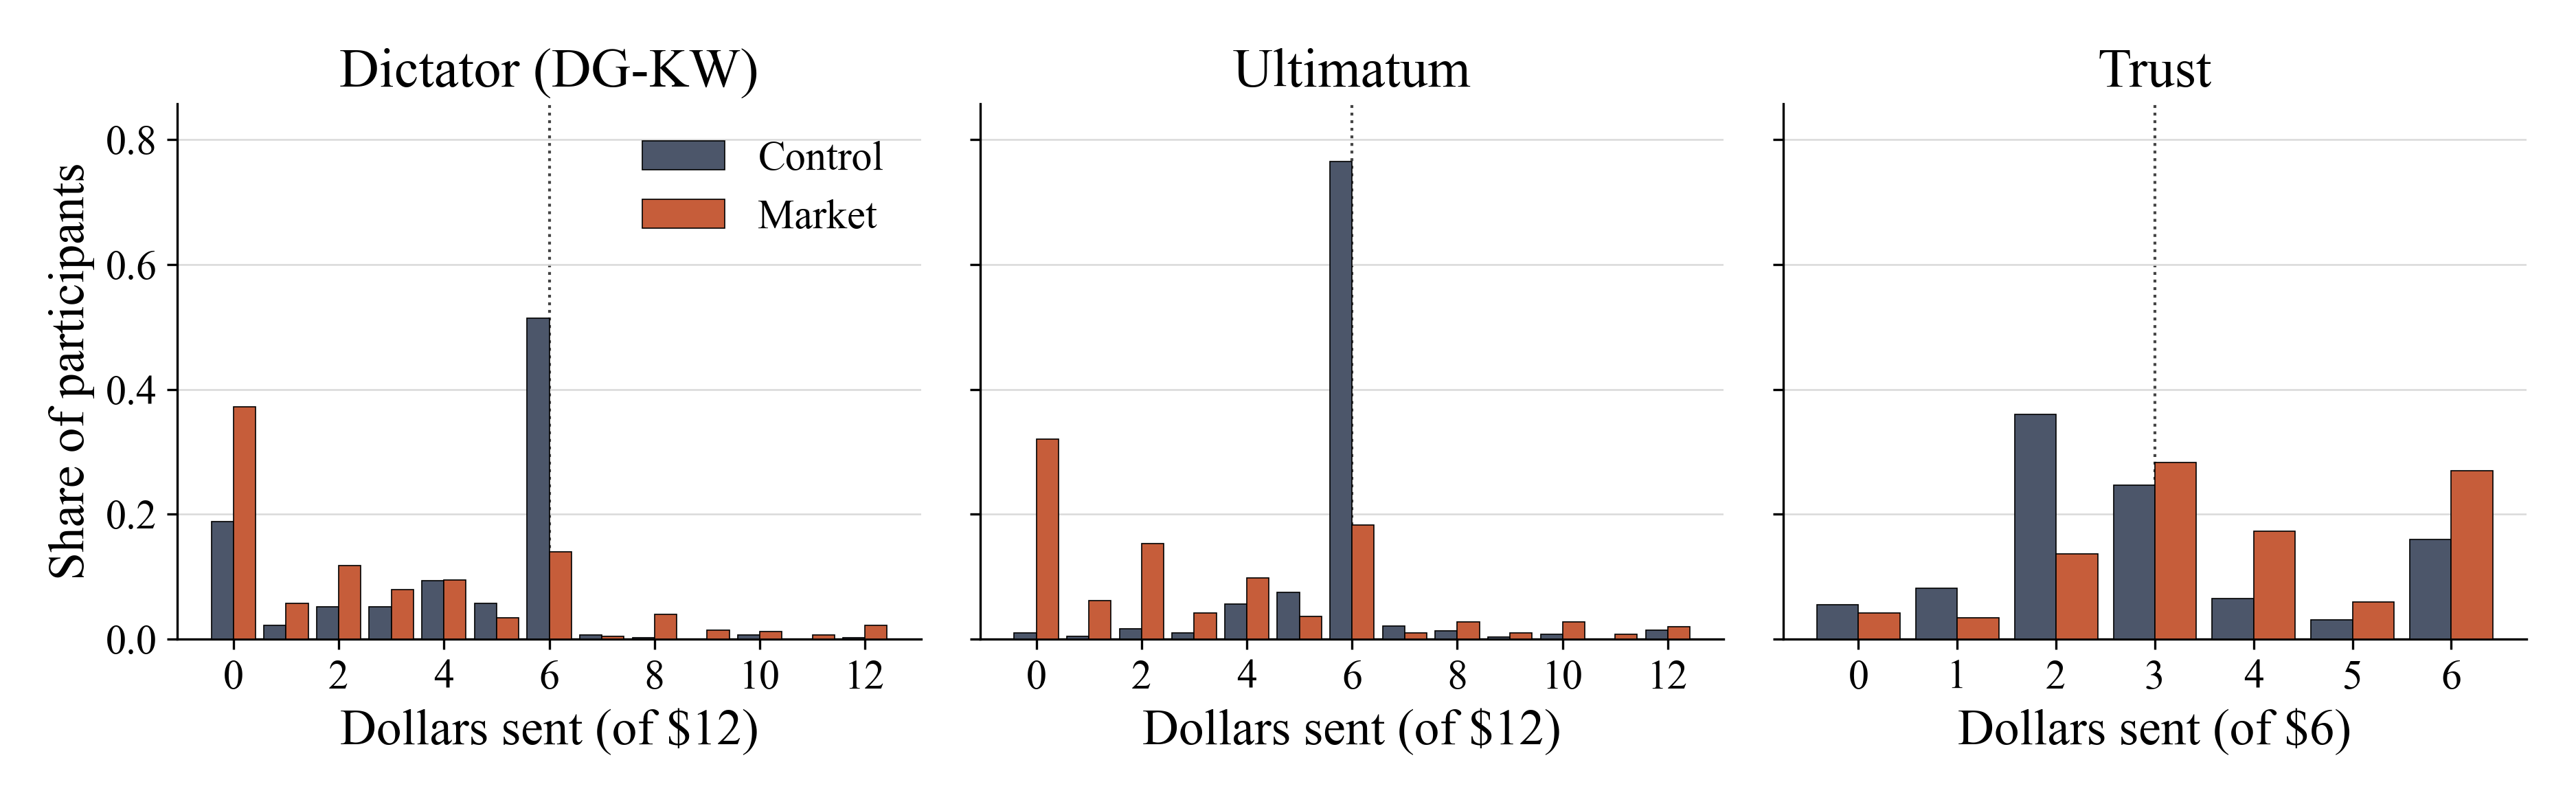
\includegraphics[width=\textwidth]{market_vs_control_distributions.png}
\caption{Distributions of Player 1 actions, Control versus Market. Bars are shares of participants at each dollar amount; the dotted line marks the equal split. Kolmogorov--Smirnov tests reject equality of the control and market distributions in every game ($D=0.32$, $0.58$, $0.28$ in DG-KW, UG, TG\@; all $p<10^{-17}$).}
\label{fig:market_distributions}
\end{figure}

The market frame is deliberately a \emph{bundle} of naturalistic cues rather than a minimal manipulation: it evokes produced---hence earned---endowments, it reframes the dictator's transfer as a price cut from an owned amount, and it gives the broker a concrete value-added role in the TG\@. Entitlement effects \citep{HoffmanMcCabeShachatSmith1994, CherryFrykblomShogren2002} are thus one ingredient of the bundle, exactly as they are in the field settings the frame imitates. The paper's claim is not that any single cue is minimal and payoff-irrelevant. It is that the bundle's effects travel through measurable representations---exactly what the category shifts, the belief shifts, and the accounting exercise of Section~\ref{sec:ge} test.

Two further features of these results resist explanations based on stable preferences plus standard channels. First, the same manipulation moves behavior in opposite directions across games (giving falls, trusting rises), which no single-dimensional shift in generosity or selfishness can produce, but which a reallocation of attention across three motives produces naturally. Second, beliefs move together with representations, strongly under the market frame and not under the stories. This contrast is consistent with the two treatments affecting different aspects of context: the stories change the narrative presented before an otherwise abstract game, whereas the market frame changes the described interaction itself. The data suggest that the latter treatment also changes how participants describe the counterpart, a possibility we examine next.
% TODO: check whether equation~\eqref{eq:retrieval} delivers this attention-vs-beliefs asymmetry formally; discuss at the coauthor call.

Changes in references to counterparts are visible in both measures. Under the market frame, the share of answers that mention no counterpart at all roughly triples in the reasons measure, from 18.5\% to 57.4\% in the DG-KW, 12.9\% to 40.5\% in the UG, and 12.2\% to 38.7\% in the TG; the hypothetical-allocation measure shows the same pattern (28.8\% to 75.9\%, Appendix~\ref{app:hp}). Together with the rise of Mutual Benefit/Cooperation, the trust-game pattern is consistent with more generalized rather than relational trust: market senders send more while describing the counterpart less often as a particular person. The measures record how participants describe the counterpart; they do not directly measure generalized trust.\footnote{\citet{GlaeserLaibsonScheinkmanSoutter2000} find that survey measures of generalized trust predict trustworthiness in the investment game better than they predict sending; \citet{Cox2004} separates trust from unconditional generosity in sending; \citet{AshrafBohnetPiankov2006} decompose trust into expectations and kindness; \citet{JohnsonMislin2011} meta-analyze 162 trust-game replications; \citet{Karlan2005} links game behavior to real repayment; \citet{Fehr2009} reviews.} The market frame changes the description of the interaction and may make a particular counterpart less salient. Where the strategic structure rewards cooperation with abstract counterparties, this abstraction need not lower sending.
% INSERTED 2026-07-16 (SP narrative per NG's 07-11 decision, market half; supersedes the Conclusions TODO on SP placement): reasons-measure no-mention shares from the SP block of output/tables/control_treatment_figure_stats.txt; hp shares recompute from tab:freqs_market_control_sp; all six trust citations verified against journal records this session.
We close the section with what the treatments do to the accuracy of beliefs; their consequences for surplus follow in Section~\ref{sec:ge}.

\subsection{Beliefs and Forecast Errors}
\label{sec:forecast}
% TODO (placement, per NG skeleton): NG's outline mentions forecast errors inside 4.1/4.2 (``maybe can already report forecast errors here''); kept as the closing subsection of Section 4 for now --- decide at the call.

Under rational expectations, context could move beliefs only by moving opponents' behavior, and forecast errors would be centered at zero in every treatment. Figure~\ref{fig:forecast_errors} shows they are not. In the UG, proposers systematically underestimate acceptance: signed forecast errors (belief minus realized Player 2 behavior) average roughly $-$17 percentage points in Control and $-$16 in the story treatments, and swing to \emph{+}9 under the market frame---proposers there expect brokers to accept even more readily than brokers actually do. Chosen-action errors condition on endogenously chosen offers, so part of the market swing reflects the shifted offer distribution; the reference-action errors in the bottom panel are immune to this selection, and there the qualitative pattern---substantial pessimism that shrinks sharply under the market frame---replicates, though the market-frame error remains mildly negative rather than turning positive. In the TG, errors are small in Control and Market ($+$1 to $+$3 points) and mildly pessimistic in the story treatments ($-$4 to $-$5 points).

\begin{figure}[!htbp]
\centering
\begin{subfigure}{0.9\textwidth}
\centering
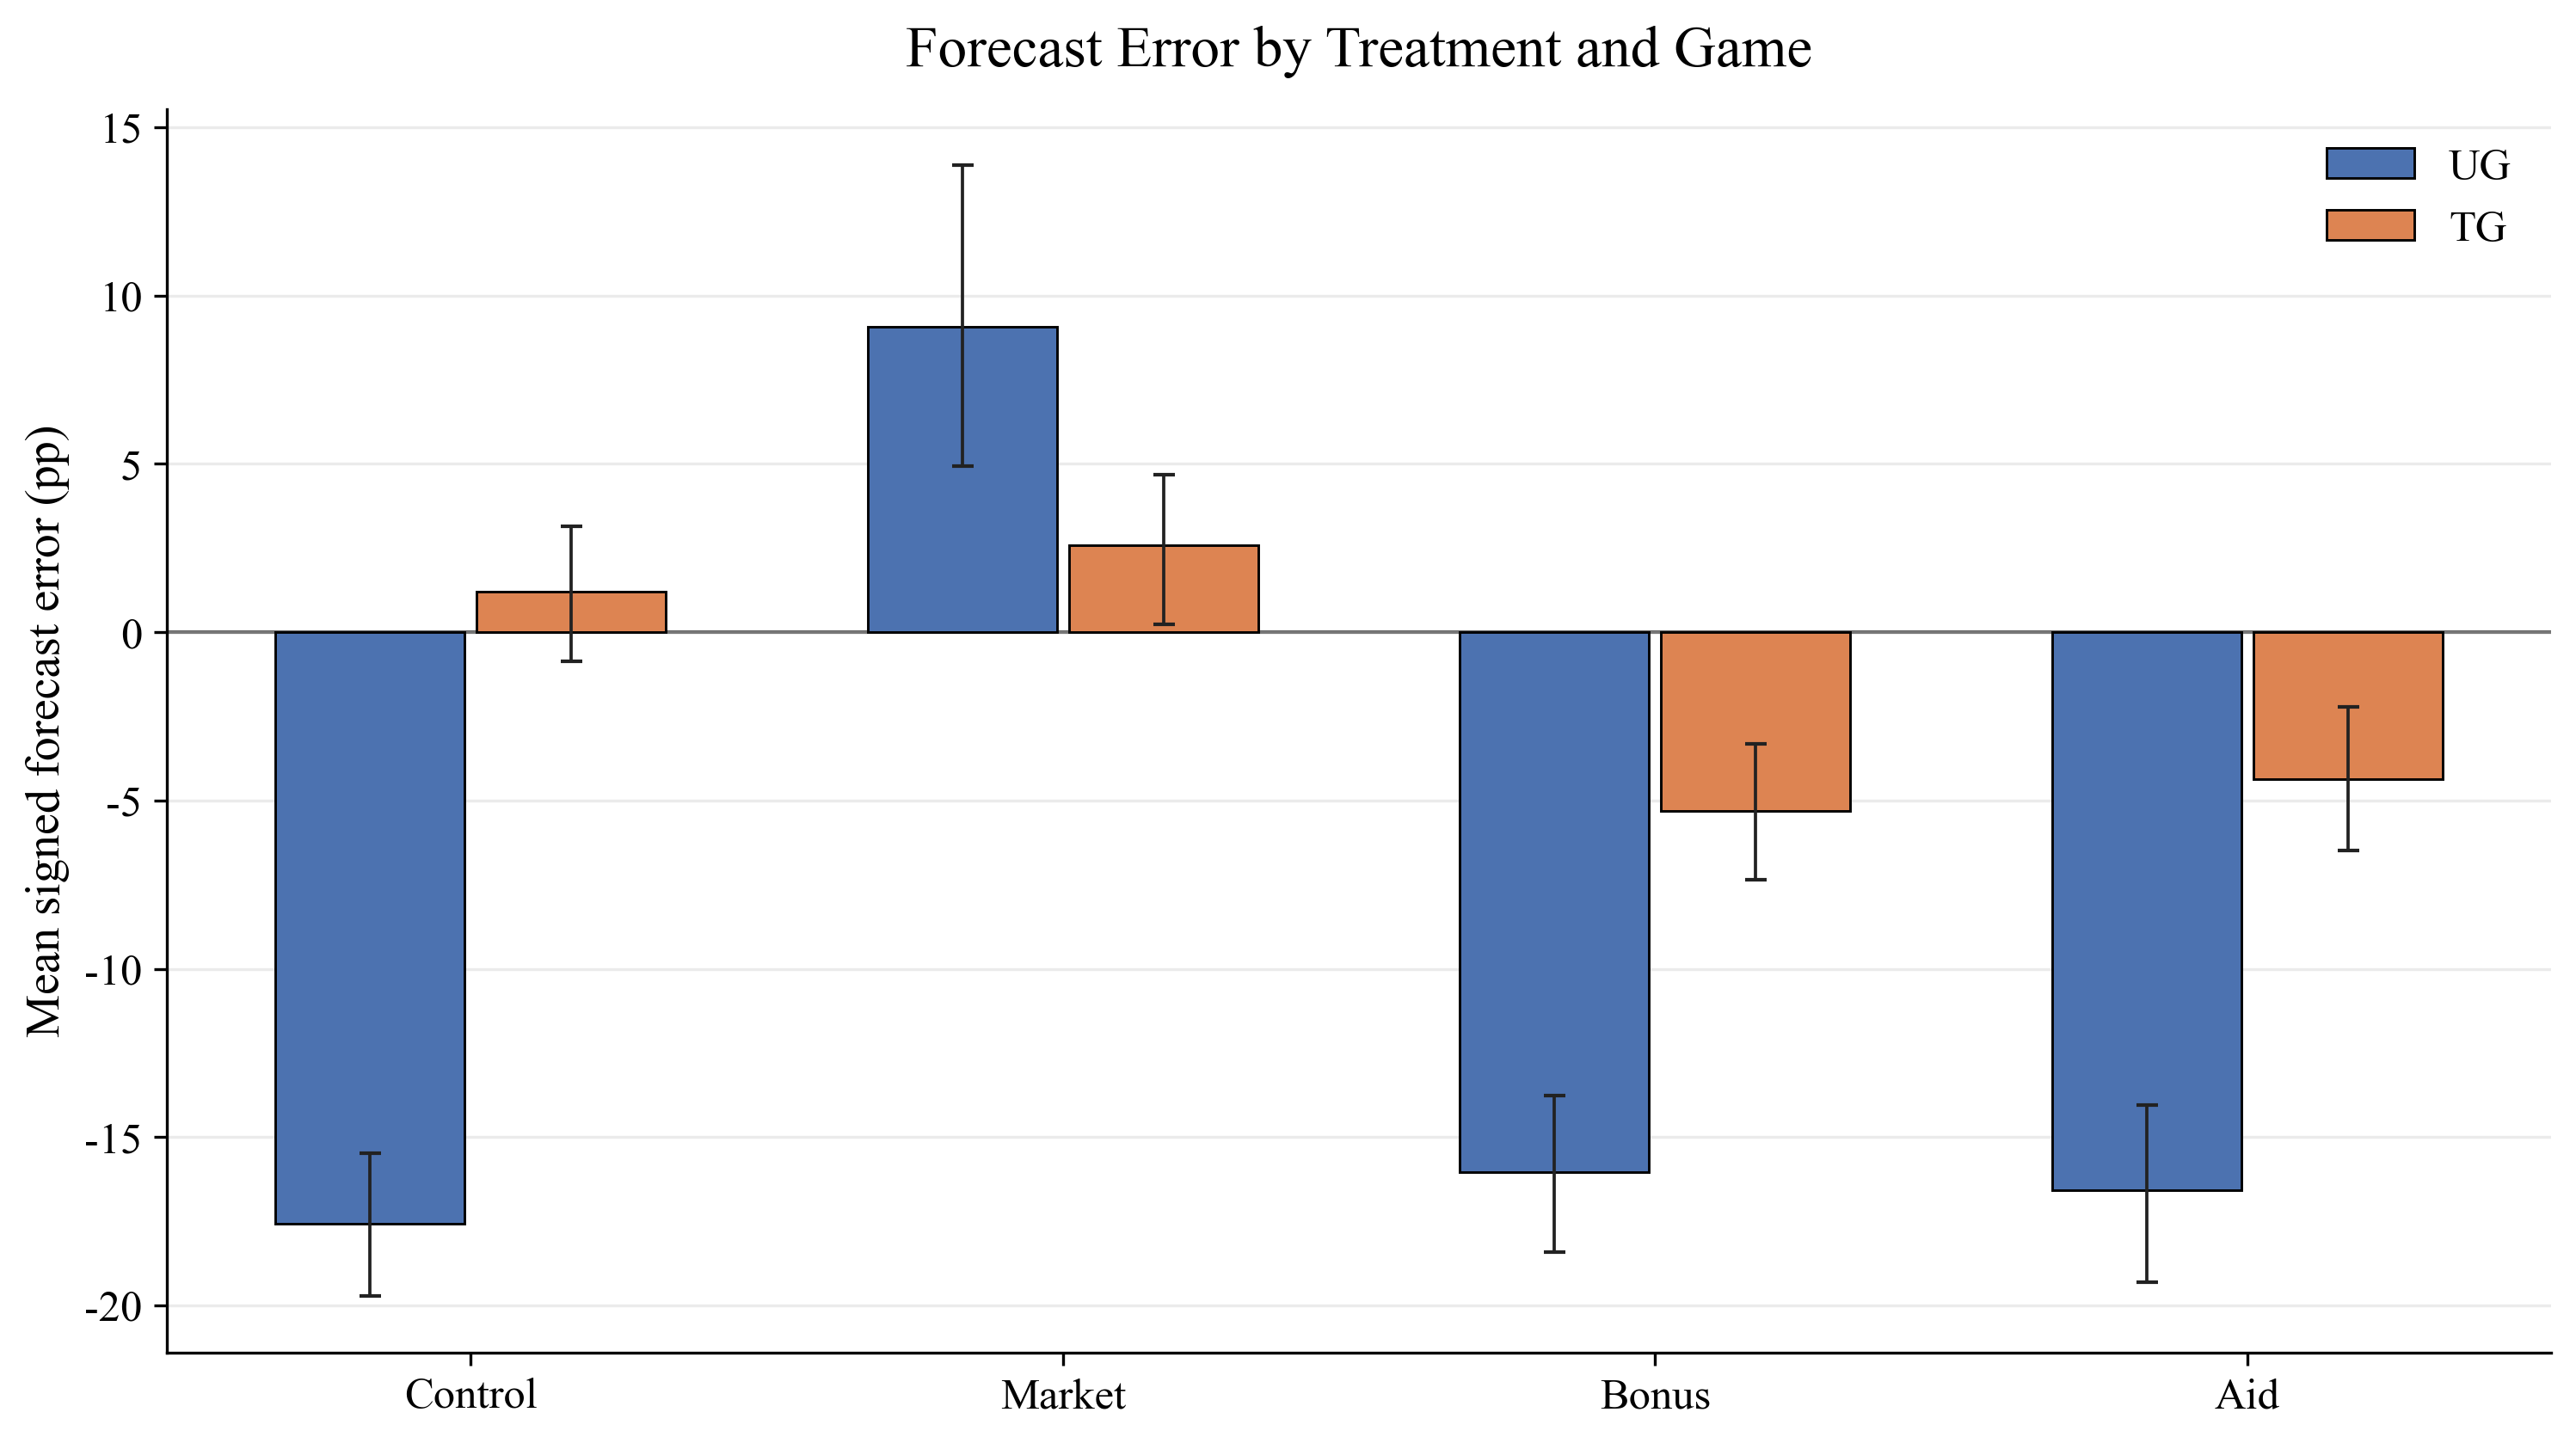
\includegraphics[width=\linewidth]{forecast_error_by_treatment.png}
\end{subfigure}

\vspace{0.35cm}

\begin{subfigure}{0.9\textwidth}
\centering
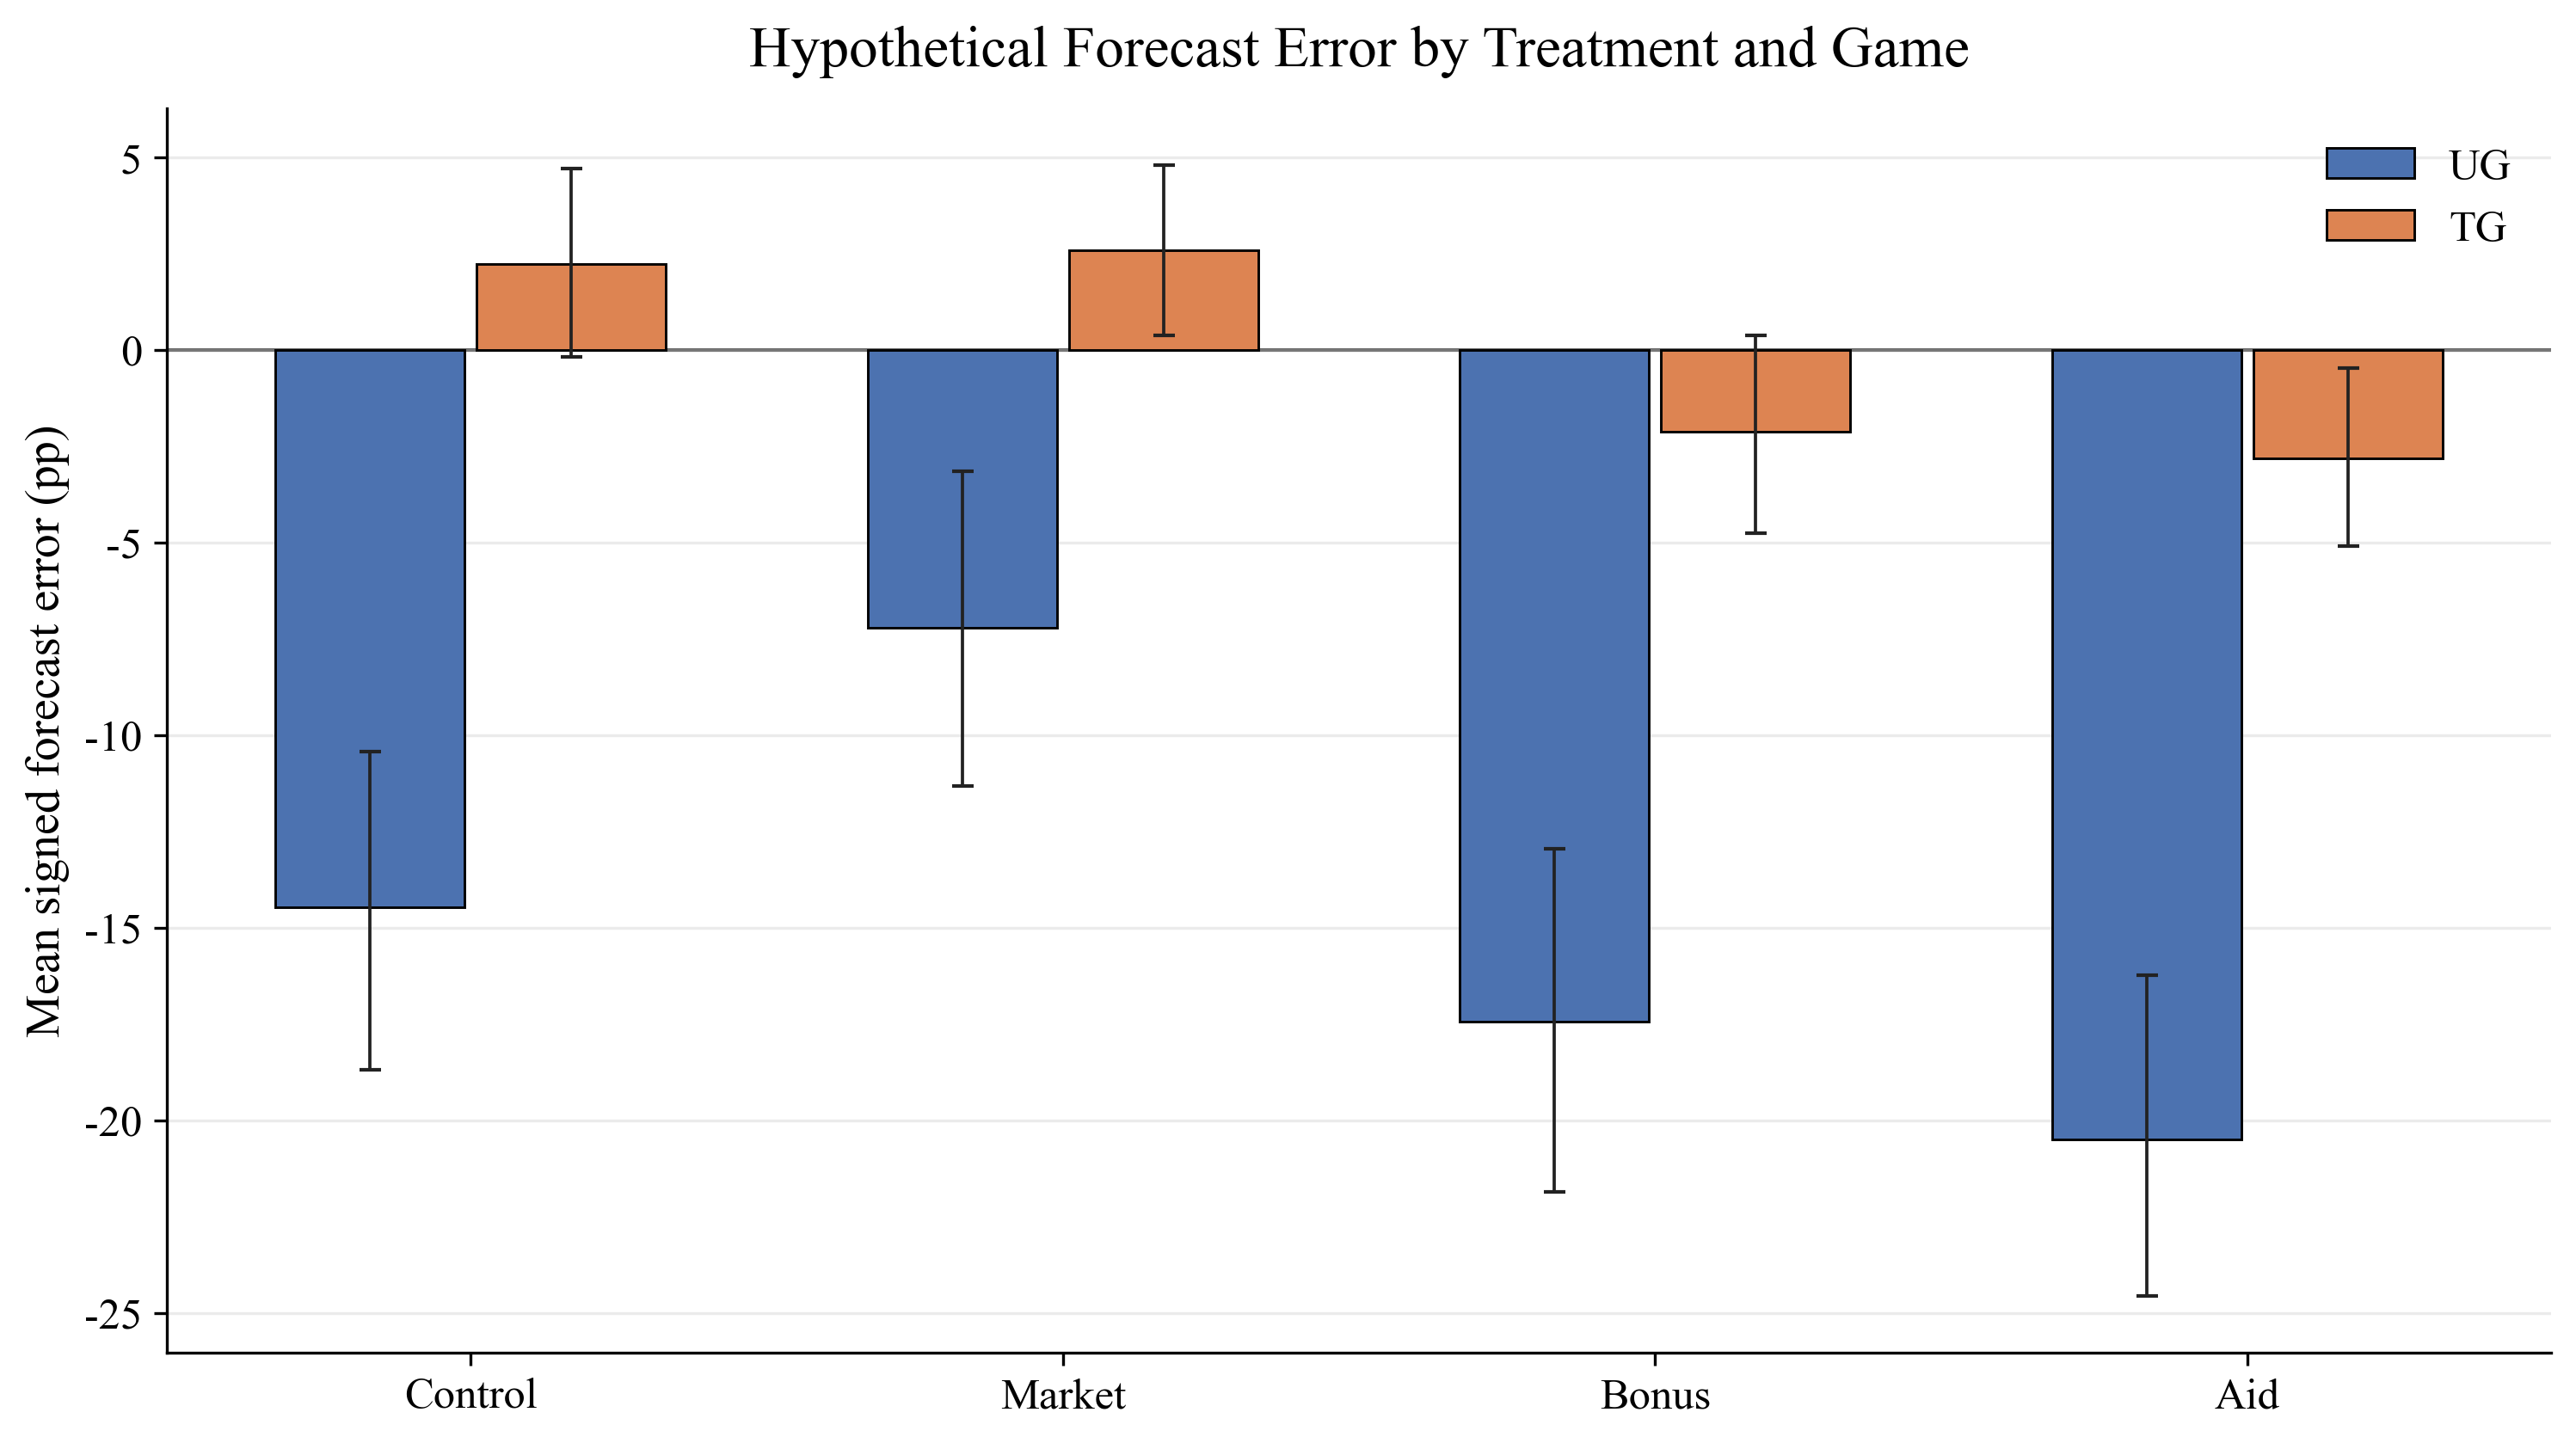
\includegraphics[width=\linewidth]{forecast_error_hp_by_treatment.png}
\end{subfigure}
\caption{Forecast errors by treatment. The top panel reports signed forecast errors for chosen-action beliefs; the benchmark is the mean realized Player 2 behavior at the same Player 1 action within the same treatment-and-game cell. The bottom panel reports signed forecast errors for hypothetical beliefs at the common one-third reference action, using the corresponding mean hypothetical Player 2 response as the benchmark. Positive values indicate optimism and negative values pessimism. Error bars show bootstrap 95\% confidence intervals.}
\label{fig:forecast_errors}
\end{figure}

% RESOLVED 2026-07-13 (AA+NG thread): receiver model inserted as Appendix app:receiver per NG's request (formalization in appendix, one-sentence pointers in the text); supersedes the 2026-07-11 "raise at the call before any paper insertion" note.
Two features tie the errors to representations. First, treatments change forecast errors, not just beliefs: the market frame moves proposers' beliefs upward by more than it moves receivers' behavior, exactly what one expects if beliefs are generated by projecting one's own (treatment-shifted) representation onto the opponent rather than by tracking the opponent's response to the same treatment. Second, within treatments, chosen-action forecast errors covary with representations: in the UG, self-interested and cooperative proposers make errors 13--16 percentage points more optimistic than moral proposers with the same hypothetical beliefs (Table~\ref{tab:cats_hp_cats_hp_fe_regs} in Appendix~\ref{app:player2}). This individual-level covariation is partly mediated by the offers those proposers choose: for reference-action errors it attenuates and, for Self-interest, reverses sign (Table~\ref{tab:cats_hp_cats_hp_hypfe_regs}), so we treat it as suggestive. The case against rational expectations rests on the first, treatment-level pattern, which survives the selection-immune measure: rational mechanisms---in which contextual cues shift equilibrium behavior and beliefs adjust correctly---cannot move mean forecast errors at all. The full model of Appendix~\ref{app:receiver} makes the pattern a prediction rather than a residual: the sender's imagined receiver and the receiver's actual behavior are retrieved from different memories given different descriptions, and nothing aligns the two retrievals, so a treatment that moves the two descriptions differently moves mean forecast errors.

These forecast errors have allocative consequences: they are how the market frame destroys surplus in the UG (Section~\ref{sec:surplus}). Receivers under the market frame are, if anything, more accepting of a given low offer (Figure~\ref{fig:player2_hypothetical}), but proposers---expecting brokers to accept even more readily than they do---cut offers so aggressively that acceptance collapses and a third of the pie is lost. In the TG, where forecast errors stay small, the same frame raises surplus. We return to these departures in the Conclusions.

\section{Explanatory Power of Representations}
\label{sec:ge}

Sections~\ref{sec:design} and~\ref{sec:treatment} establish the two links of the proposed chain separately: representations predict behavior within a context, and randomized context shifts representations. This section combines them. Section~\ref{sec:heterogeneity} asks whether measured representation shifts, weighted by how each representation behaves, quantitatively account for treatment effects---on actions and beliefs, for both players---and for the heterogeneity and allocative consequences behind the means. Section~\ref{sec:kwlt} then returns to the puzzle that opened the paper and reads it with the same instruments.

\subsection{Heterogeneity and Instability}
\label{sec:heterogeneity}

\paragraph{Second movers.}
\label{sec:p2_hypothetical}
% DECIDED 2026-07-13 (AA+NG thread): the main text shows only Player 2 hypothetical behavior before the regressions (AA: the only clean partial-equilibrium outcome for the receiver; NG: "partiamo mostrando solo hypothetical beliefs mettendo le altre figure in appendice, poi vediamo"); category shifts and all other Player 2 figures in Appendix app:player2. Figure produced by 07_player2_exhibit_split.py --- a pure re-layout of appendix_player2_treatment_effects.png rows, no new statistics.
Before the regressions, we bring in the second movers. They enter through their \emph{hypothetical} responses---acceptance of a given offer, return of a given send---because these are their only clean partial-equilibrium outcomes: realized acceptance and returns respond to endogenously chosen first-mover actions, and even measured representations are elicited after the receiver faces the action, which may itself cue her retrieval (Appendix~\ref{app:receiver}). Figure~\ref{fig:player2_hypothetical} reports treatment effects on hypothetical outcomes at the one-third reference action, together with the treatment-level means of the hypothetical actions. The market frame crowds out receivers' \emph{Moral good} representations in favor of Self-interest and \emph{Moral bad} (Figure~\ref{fig:appendix_player2_category_shifts} in Appendix~\ref{app:player2}), yet both hypothetical acceptance of a one-third offer and trustees' hypothetical returns \emph{rise} by about 10 points---the mirror image of the sender-side pattern, and the reason realized surplus moves as it does below. Control-sample distributions, category--outcome associations, and the underlying regressions are in Appendix~\ref{app:player2}.

\begin{figure}[!htbp]
\centering
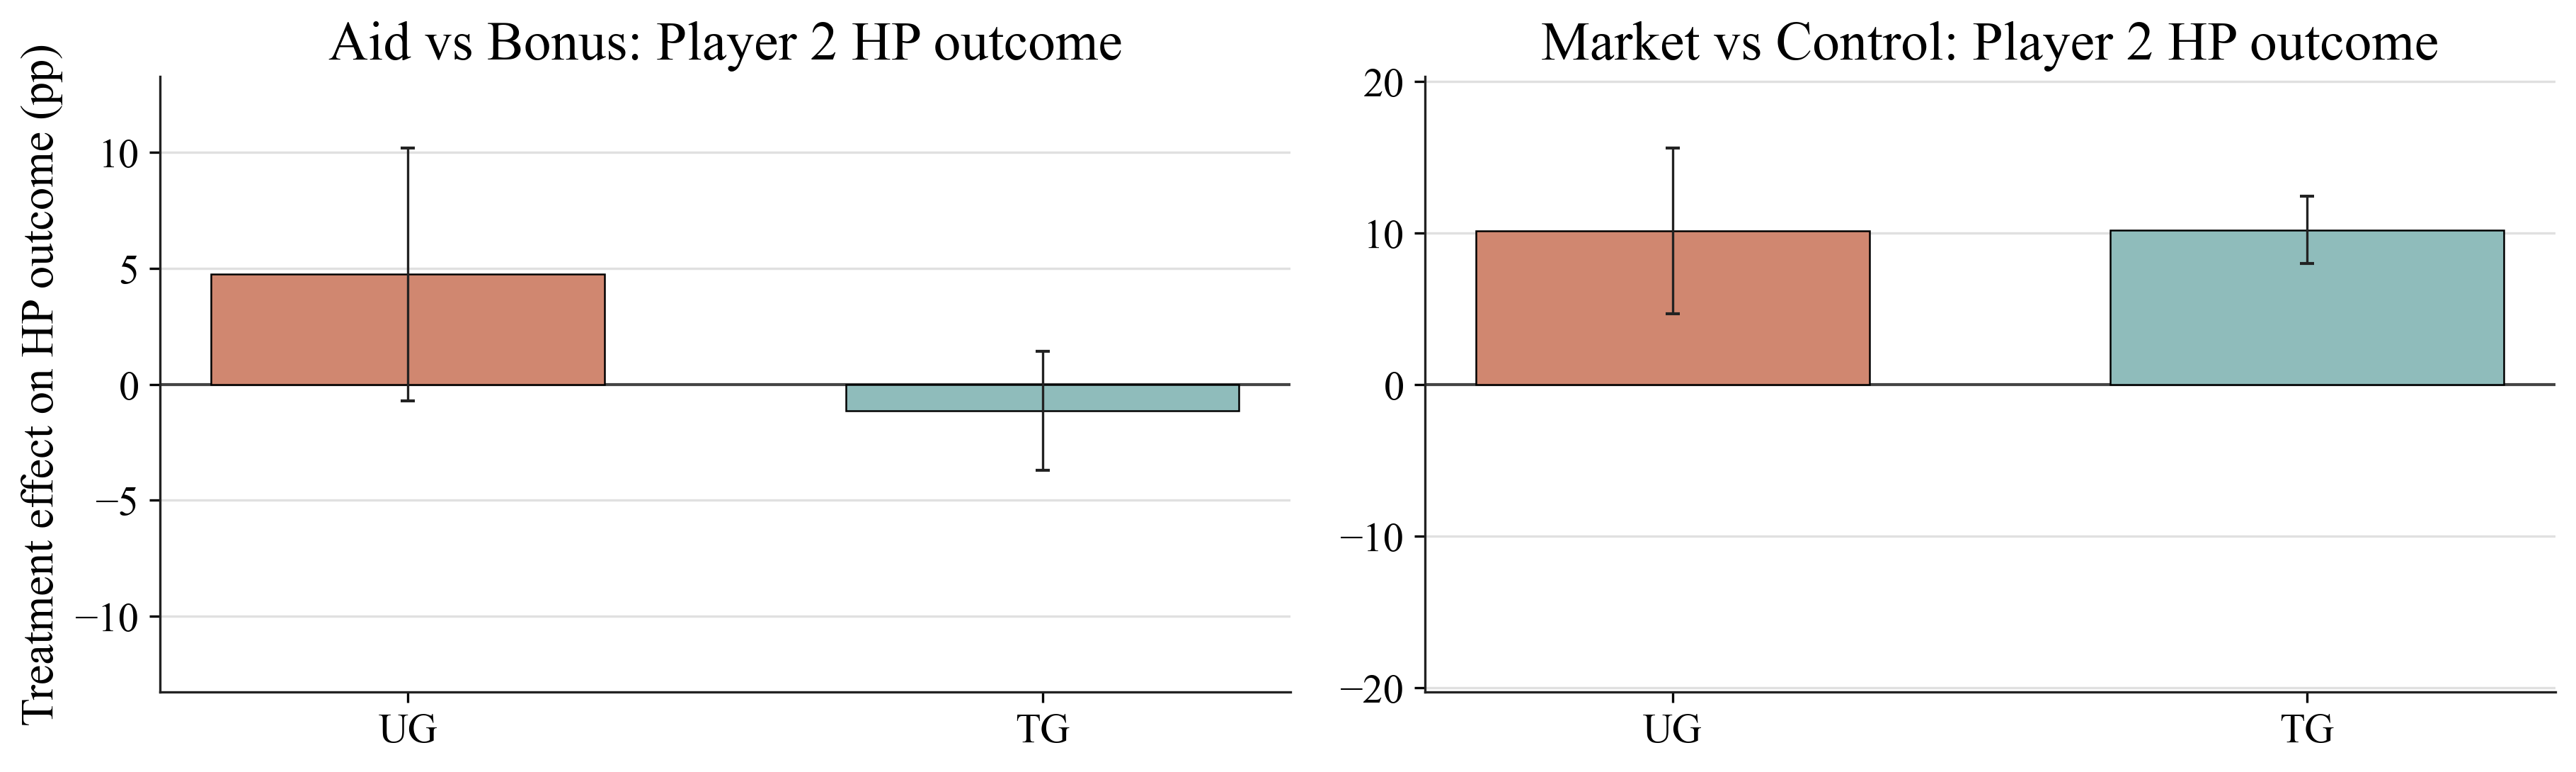
\includegraphics[width=0.96\textwidth]{player2_hypothetical_treatment_effects.png}
\caption{Player 2 hypothetical behavior. Columns report Aid vs Bonus and Market vs Control. The top row shows treatment effects on hypothetical outcomes; a model-predicted direction marker appears only when the effect is statistically distinguishable from zero and the model prediction is unambiguous. The bottom row reports the treatment-level means of Player 2 hypothetical actions in UG and TG\@. Error bars show 95\% confidence intervals.}
\label{fig:player2_hypothetical}
\end{figure}

\paragraph{Benchmark regressions.}
\label{sec:benchmark}
The benchmark regressions estimate the association between representation categories and each outcome---the per-category behavior that, combined with the treatment-induced category shifts, generates the predictions of the accounting exercise below. For each pre-registered comparison (Aid vs Bonus; Market vs Control) we pool the two arms and, separately by game, regress Player 1 outcomes on category dummies, adding hypothetical beliefs for UG offers, TG sends, and the belief outcomes to capture the belief channel of Section~\ref{sec:model}. For Player 2, we regress UG acceptance and TG returns on category dummies plus the participant's hypothetical response at the reference action; a second specification adds the fitted Player 1 action, because realized acceptance and returns conflate second movers' standards with treatment-shifted first-mover behavior. The belief outcomes in the Player 1 regressions and in the fit exercise below are chosen-action beliefs. Tables~\ref{tab:cats_hp_aid_vs_bonus_fullpooled_p1_regs}--\ref{tab:cats_hp_market_vs_control_fullpooled_p2_regs} report the estimates.

The coefficients quantify the control-sample patterns: category gaps are large where representations bite and small where strategic discipline mutes them. Self-interest (relative to Moral) is associated with dictator transfers 30--34 percentage points lower, but with UG offers only 12--16 points lower; Mutual Benefit/Cooperation is associated with TG sends 24--33 points higher. Among second movers, Moral bad is the dominant predictor, associated with acceptance 84--91 percentage points lower and returns 28--29 points lower. Beliefs enter exactly where the model says they should: hypothetical beliefs predict TG sends strongly (coefficients 0.24--0.36) and enter UG offers with the opposite, model-consistent sign ($-0.04$ to $-0.15$)---a proposer who believes a low offer would be accepted offers less. These are exactly the belief-channel signs of equations~\eqref{eq:ug_offer} and~\eqref{eq:tg_send}, and their opposite signs across the two games are a joint prediction no belief-free account shares.

\begin{table}[!htbp]
\centering
\caption{\textbf{Benchmark Regressions: Player 1, Aid vs Bonus, Categories + Beliefs HP}}
\label{tab:cats_hp_aid_vs_bonus_fullpooled_p1_regs}
\resizebox{0.98\textwidth}{!}{%
\begin{tabular}{lccccc}
\toprule
 & (1) & (2) & (3) & (4) & (5) \\
 & KW action & UG action & TG action & UG beliefs & TG beliefs \\
\midrule
Self-interest & -0.337$^{***}$ & -0.124$^{***}$ & -0.151$^{***}$ & -0.159$^{***}$ & -0.031$^{**}$ \\
 & (0.010) & (0.009) & (0.024) & (0.016) & (0.015) \\
Mutual Benefit / Cooperation & 0.011 & 0.059$^{***}$ & 0.326$^{***}$ & 0.040 & 0.106$^{***}$ \\
 & (0.033) & (0.016) & (0.017) & (0.028) & (0.010) \\
No clear justification & -0.245$^{***}$ & -0.032 & -0.035 & -0.210$^{***}$ & 0.015 \\
 & (0.036) & (0.024) & (0.077) & (0.041) & (0.047) \\
Hypothetical beliefs &  & -0.038$^{**}$ & 0.240$^{***}$ & 0.345$^{***}$ & 0.574$^{***}$ \\
 &  & (0.015) & (0.042) & (0.026) & (0.026) \\
Constant & 0.457$^{***}$ & 0.512$^{***}$ & 0.380$^{***}$ & 0.629$^{***}$ & 0.117$^{***}$ \\
 & (0.005) & (0.008) & (0.018) & (0.014) & (0.011) \\
\midrule
Observations & 801 & 1142 & 947 & 1142 & 947 \\
$R^2$ & 0.599 & 0.162 & 0.407 & 0.193 & 0.436 \\
\bottomrule
\end{tabular}
}
\begin{flushleft}
\footnotesize Standard errors in parentheses. Baseline category is Moral. Sample restricted to Bonus and Aid. UG and TG equations include hypothetical beliefs in addition to category dummies; KW action uses category dummies only. $^{*}p<0.10$, $^{**}p<0.05$, $^{***}p<0.01$.
\end{flushleft}
\end{table}

\begin{table}[!htbp]
\centering
\caption{\textbf{Benchmark Regressions: Player 2, Aid vs Bonus, Categories + Beliefs HP}}
\label{tab:cats_hp_aid_vs_bonus_fullpooled_p2_regs}
\resizebox{0.94\textwidth}{!}{%
\begin{tabular}{lcccc}
\toprule
 & (1) & (2) & (3) & (4) \\
 & UG outcome & TG outcome & UG outcome + fitted share sent P1 & TG outcome + fitted share sent P1 \\
\midrule
Moral bad & -0.844$^{***}$ & -0.294$^{***}$ & -0.746$^{***}$ & -0.212$^{***}$ \\
 & (0.024) & (0.020) & (0.029) & (0.019) \\
Mutual Benefit / Cooperation & 0.004 & 0.004 & 0.011 & 0.001 \\
 & (0.012) & (0.011) & (0.011) & (0.010) \\
No clear justification & -0.016 & -0.093$^{**}$ & -0.002 & -0.067$^{*}$ \\
 & (0.034) & (0.038) & (0.033) & (0.034) \\
Self-interest & -0.062$^{***}$ & -0.178$^{***}$ & -0.032$^{*}$ & -0.162$^{***}$ \\
 & (0.016) & (0.020) & (0.016) & (0.018) \\
Hypothetical acceptance & 0.027$^{**}$ &  & 0.031$^{***}$ &  \\
 & (0.011) &  & (0.011) &  \\
Hypothetical share sent P2 &  & 0.516$^{***}$ &  & 0.504$^{***}$ \\
 &  & (0.025) &  & (0.023) \\
Predicted share sent P1 &  &  & 1.259$^{***}$ & 0.558$^{***}$ \\
 &  &  & (0.220) & (0.040) \\
Constant & 0.964$^{***}$ & 0.236$^{***}$ & 0.350$^{***}$ & -0.089$^{***}$ \\
 & (0.010) & (0.011) & (0.108) & (0.025) \\
\midrule
Observations & 1142 & 923 & 1142 & 923 \\
$R^2$ & 0.529 & 0.497 & 0.542 & 0.585 \\
\bottomrule
\end{tabular}
}
\begin{flushleft}
\footnotesize Standard errors in parentheses. Baseline category is Moral good. Sample restricted to Bonus and Aid. Columns (3) and (4) add fitted share sent P1, computed from the comparison-specific Player 1 action regression in the same specification by averaging fitted values within each observed Player 1 donation level. UG equations include hypothetical acceptance and TG equations include hypothetical share sent P2; columns (3) and (4) additionally include fitted share sent P1. $^{*}p<0.10$, $^{**}p<0.05$, $^{***}p<0.01$.
\end{flushleft}
\end{table}


\clearpage

\begin{table}[!htbp]
\centering
\caption{\textbf{Benchmark Regressions: Player 1, Market vs Control, Categories + Beliefs HP}}
\label{tab:cats_hp_market_vs_control_fullpooled_p1_regs}
\resizebox{0.98\textwidth}{!}{%
\begin{tabular}{lccccc}
\toprule
 & (1) & (2) & (3) & (4) & (5) \\
 & KW action & UG action & TG action & UG beliefs & TG beliefs \\
\midrule
Self-interest & -0.299$^{***}$ & -0.164$^{***}$ & -0.083$^{***}$ & -0.093$^{***}$ & 0.001 \\
 & (0.016) & (0.016) & (0.022) & (0.015) & (0.013) \\
Mutual Benefit / Cooperation & -0.082$^{***}$ & -0.162$^{***}$ & 0.244$^{***}$ & -0.066$^{***}$ & 0.080$^{***}$ \\
 & (0.027) & (0.020) & (0.019) & (0.018) & (0.011) \\
No clear justification & -0.211$^{***}$ & -0.197$^{***}$ & 0.074$^{*}$ & -0.148$^{***}$ & 0.067$^{***}$ \\
 & (0.025) & (0.022) & (0.041) & (0.021) & (0.023) \\
Hypothetical beliefs &  & -0.148$^{***}$ & 0.364$^{***}$ & 0.281$^{***}$ & 0.674$^{***}$ \\
 &  & (0.027) & (0.038) & (0.025) & (0.022) \\
Constant & 0.418$^{***}$ & 0.543$^{***}$ & 0.368$^{***}$ & 0.629$^{***}$ & 0.100$^{***}$ \\
 & (0.010) & (0.017) & (0.020) & (0.016) & (0.011) \\
\midrule
Observations & 803 & 1137 & 1011 & 1137 & 1011 \\
$R^2$ & 0.324 & 0.179 & 0.330 & 0.129 & 0.542 \\
\bottomrule
\end{tabular}
}
\begin{flushleft}
\footnotesize Standard errors in parentheses. Baseline category is Moral. Sample restricted to Control and Market. UG and TG equations include hypothetical beliefs in addition to category dummies; KW action uses category dummies only. $^{*}p<0.10$, $^{**}p<0.05$, $^{***}p<0.01$.
\end{flushleft}
\end{table}

\begin{table}[!htbp]
\centering
\caption{\textbf{Benchmark Regressions: Player 2, Market vs Control, Categories + Beliefs HP}}
\label{tab:cats_hp_market_vs_control_fullpooled_p2_regs}
\resizebox{0.94\textwidth}{!}{%
\begin{tabular}{lcccc}
\toprule
 & (1) & (2) & (3) & (4) \\
 & UG outcome & TG outcome & UG outcome + fitted share sent P1 & TG outcome + fitted share sent P1 \\
\midrule
Moral bad & -0.906$^{***}$ & -0.280$^{***}$ & -0.724$^{***}$ & -0.230$^{***}$ \\
 & (0.033) & (0.022) & (0.035) & (0.023) \\
Mutual Benefit / Cooperation & -0.057$^{**}$ & -0.011 & -0.022 & -0.007 \\
 & (0.024) & (0.010) & (0.023) & (0.010) \\
No clear justification & -0.243$^{***}$ & -0.024 & -0.157$^{***}$ & -0.025 \\
 & (0.055) & (0.021) & (0.053) & (0.021) \\
Self-interest & -0.302$^{***}$ & -0.148$^{***}$ & -0.161$^{***}$ & -0.152$^{***}$ \\
 & (0.024) & (0.015) & (0.026) & (0.015) \\
Hypothetical acceptance & 0.038$^{*}$ &  & 0.071$^{***}$ &  \\
 & (0.020) &  & (0.019) &  \\
Hypothetical share sent P2 &  & 0.529$^{***}$ &  & 0.504$^{***}$ \\
 &  & (0.026) &  & (0.025) \\
Predicted share sent P1 &  &  & 1.738$^{***}$ & 0.445$^{***}$ \\
 &  &  & (0.160) & (0.054) \\
Constant & 0.951$^{***}$ & 0.226$^{***}$ & 0.206$^{***}$ & -0.039 \\
 & (0.019) & (0.012) & (0.071) & (0.035) \\
\midrule
Observations & 1137 & 1016 & 1137 & 964 \\
$R^2$ & 0.432 & 0.481 & 0.486 & 0.515 \\
\bottomrule
\end{tabular}
}
\begin{flushleft}
\footnotesize Standard errors in parentheses. Baseline category is Moral good. Sample restricted to Control and Market. Columns (3) and (4) add fitted share sent P1, computed from the comparison-specific Player 1 action regression in the same specification by averaging fitted values within each observed Player 1 donation level. UG equations include hypothetical acceptance and TG equations include hypothetical share sent P2; columns (3) and (4) additionally include fitted share sent P1. $^{*}p<0.10$, $^{**}p<0.05$, $^{***}p<0.01$.
\end{flushleft}
\end{table}



\paragraph{Predicted versus actual treatment effects.}
\label{sec:predicted_actual}
We then combine each benchmark regression with the treatment-induced shifts in its regressors---category shares and, where included, hypothetical beliefs (for Player 2, also the fitted Player 1 action)---to \emph{predict} the treatment effect on each outcome, and compare the prediction with the actual effect. This is a demanding exercise: the benchmark coefficients are identified mostly from within-arm heterogeneity, and the prediction uses only the movement of measured representations and beliefs across arms.

Figures~\ref{fig:instability_p1}--\ref{fig:instability_p2_hyp} plot predicted against actual effects for Player 1 actions, Player 1 beliefs, Player 2 outcomes, and Player 2 hypothetical actions; Table~\ref{tab:cats_hp_instability_regs} reports the calibration regressions. Three findings stand out. First, predicted and actual effects agree in sign in 17 of the 18 cells, including every action cell---and including the reversal between UG offers (down under Market) and TG sends (up under Market). The single sign miss is a belief cell: the model predicts essentially no effect of the market frame on proposers' chosen-action acceptance beliefs ($+0.003$), while the actual effect is negative ($-0.062$).\footnote{Treatment effects on beliefs in Section~\ref{sec:treatment} refer to hypothetical beliefs at the reference action; the belief cells in the fit exercise are chosen-action beliefs, so magnitudes are not comparable across the two.} Second, the fit is tight: regressing actual on predicted effects across all 18 outcome-by-comparison cells yields a slope of 1.24 and $R^{2}=0.87$ (Player 1: slope 1.77, $R^{2}=0.95$; Player 2: slope 1.10, $R^{2}=0.92$). We read slope and $R^{2}$ as descriptive fit statistics: the cells are estimated from overlapping samples, so the conventional standard errors in Table~\ref{tab:cats_hp_instability_regs} are indicative at best.\footnote{Categories alone, without the belief channel, already deliver $R^{2}=0.80$ with slope 1.41 (Player 1 alone: slope 2.77), so the accounting power does not hinge on beliefs; beliefs mainly improve the fit for the trust game. See Table~\ref{tab:cats_only_instability_regs} in Appendix~\ref{app:player2}. For Player 2, a variant that replaces the fitted Player 1 action with the representation-\emph{predicted} Player 1 action---so that no actual treatment variation in first-mover behavior enters the prediction---delivers similar or better fit (predicted-to-actual ratio 0.88 versus 0.62 for UG acceptance under the market comparison). % TODO: consider surfacing the predicted-sender variant as the headline Player 2 specification.
} Third, predicted magnitudes fall short of actual ones (predicted-to-actual ratios of roughly 0.5 for the large first-mover effects). Coarse categories measuring the underlying attention weights with classical error would produce exactly this attenuation, and the pre-choice measure of Appendix~\ref{app:hp} supports that reading; measurement error of the rationalization type would push the other way, however, so we read the ratios as descriptive rather than as bounds.

\begin{figure}[!htbp]
\centering
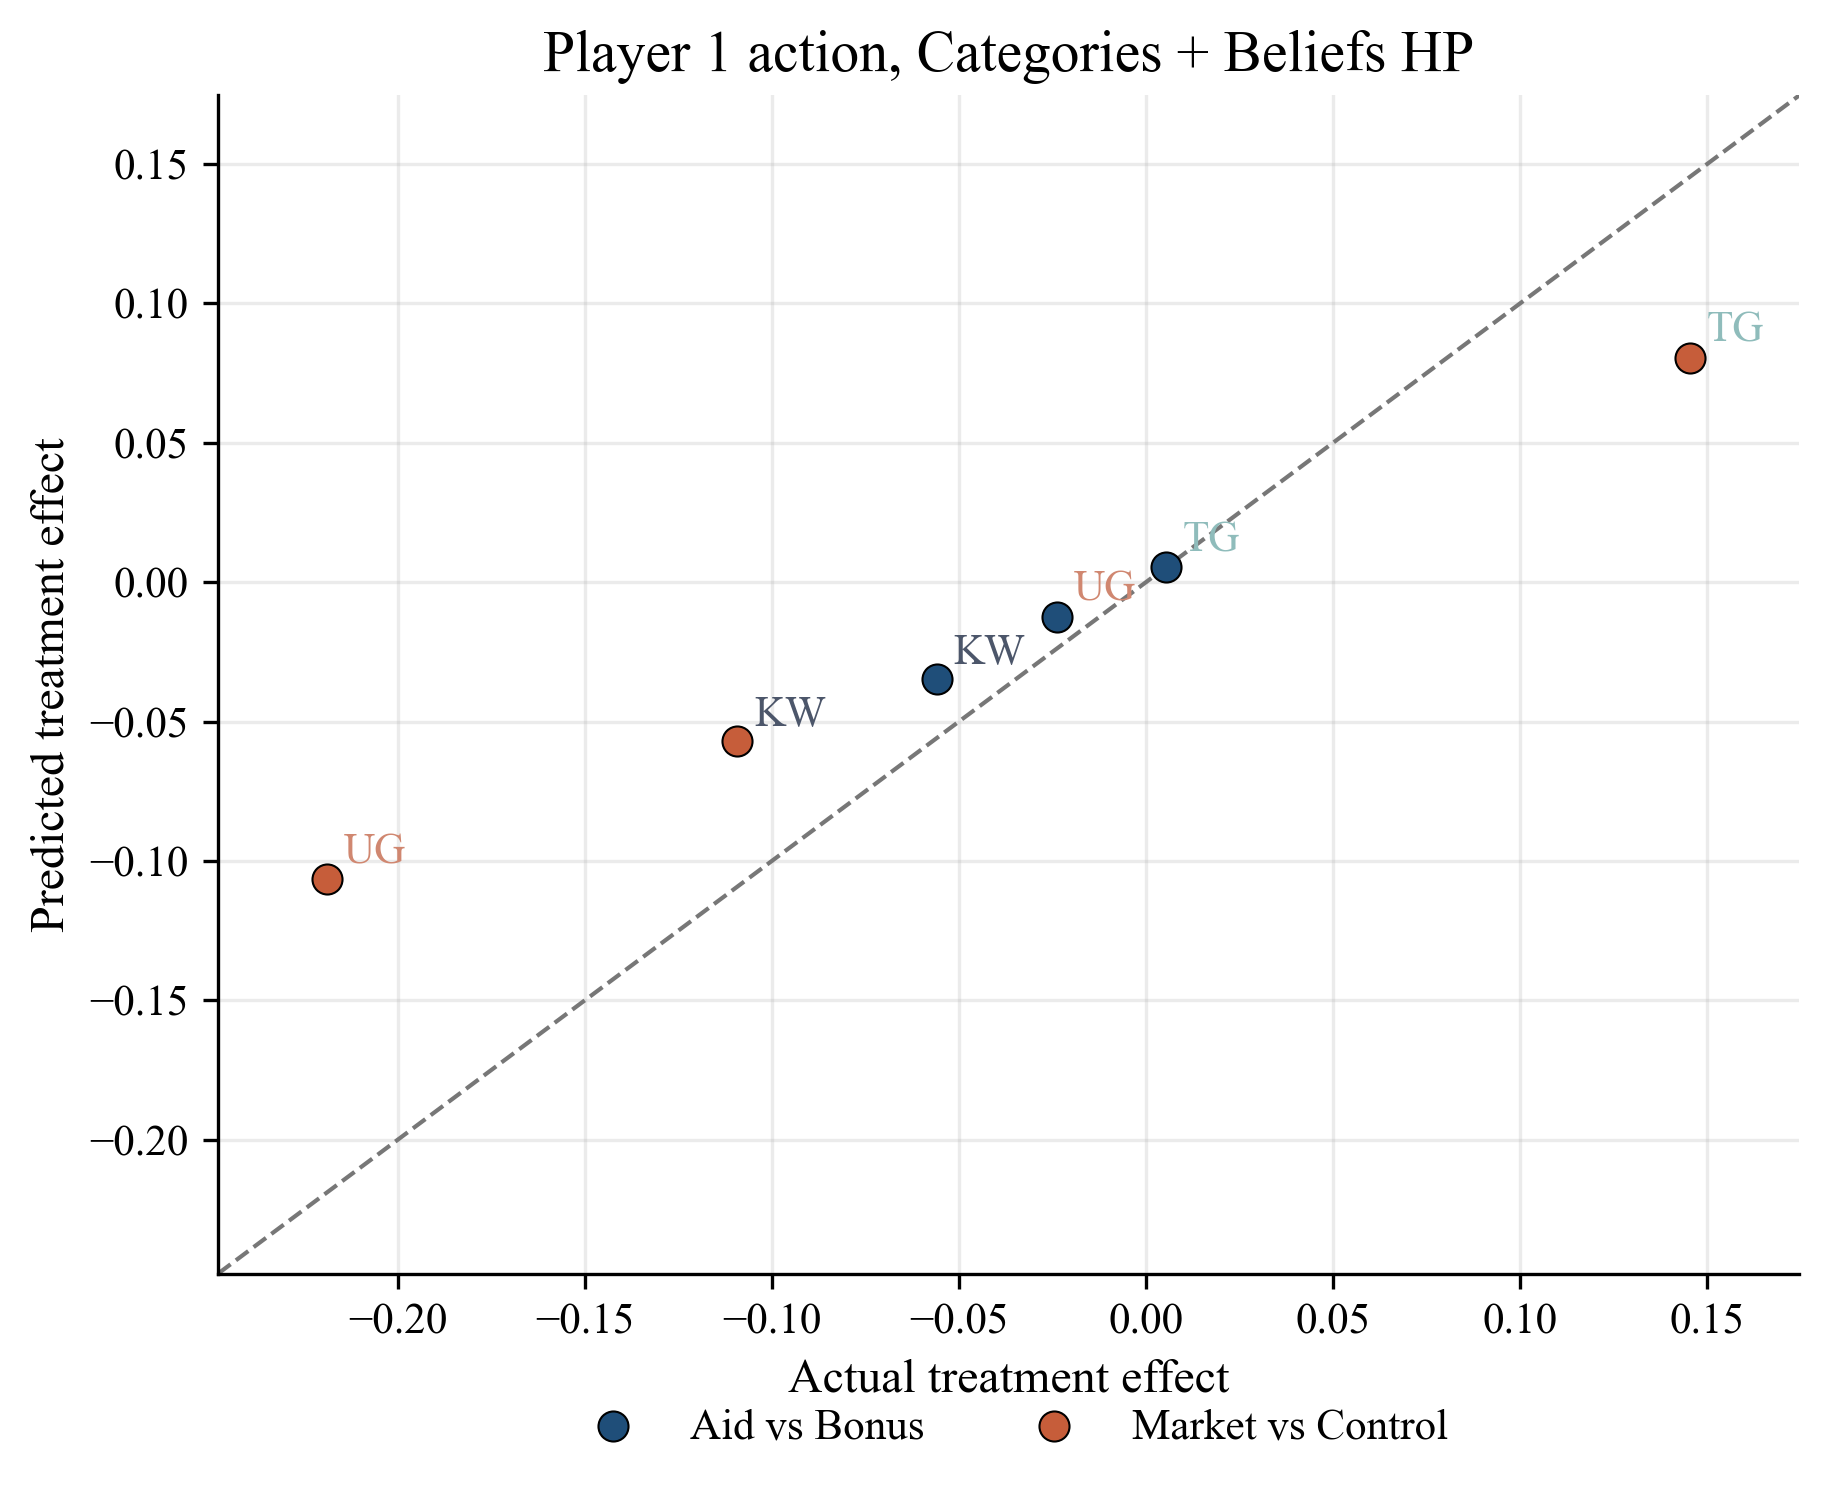
\includegraphics[width=0.74\textwidth]{cats_hp_instability_p1.png}
\caption{Predicted vs actual treatment effects for Player 1 actions, Categories + Beliefs specification. Each point is an outcome-by-comparison cell; the 45-degree line marks exact fit.}
\label{fig:instability_p1}
\end{figure}

\begin{figure}[!htbp]
\centering
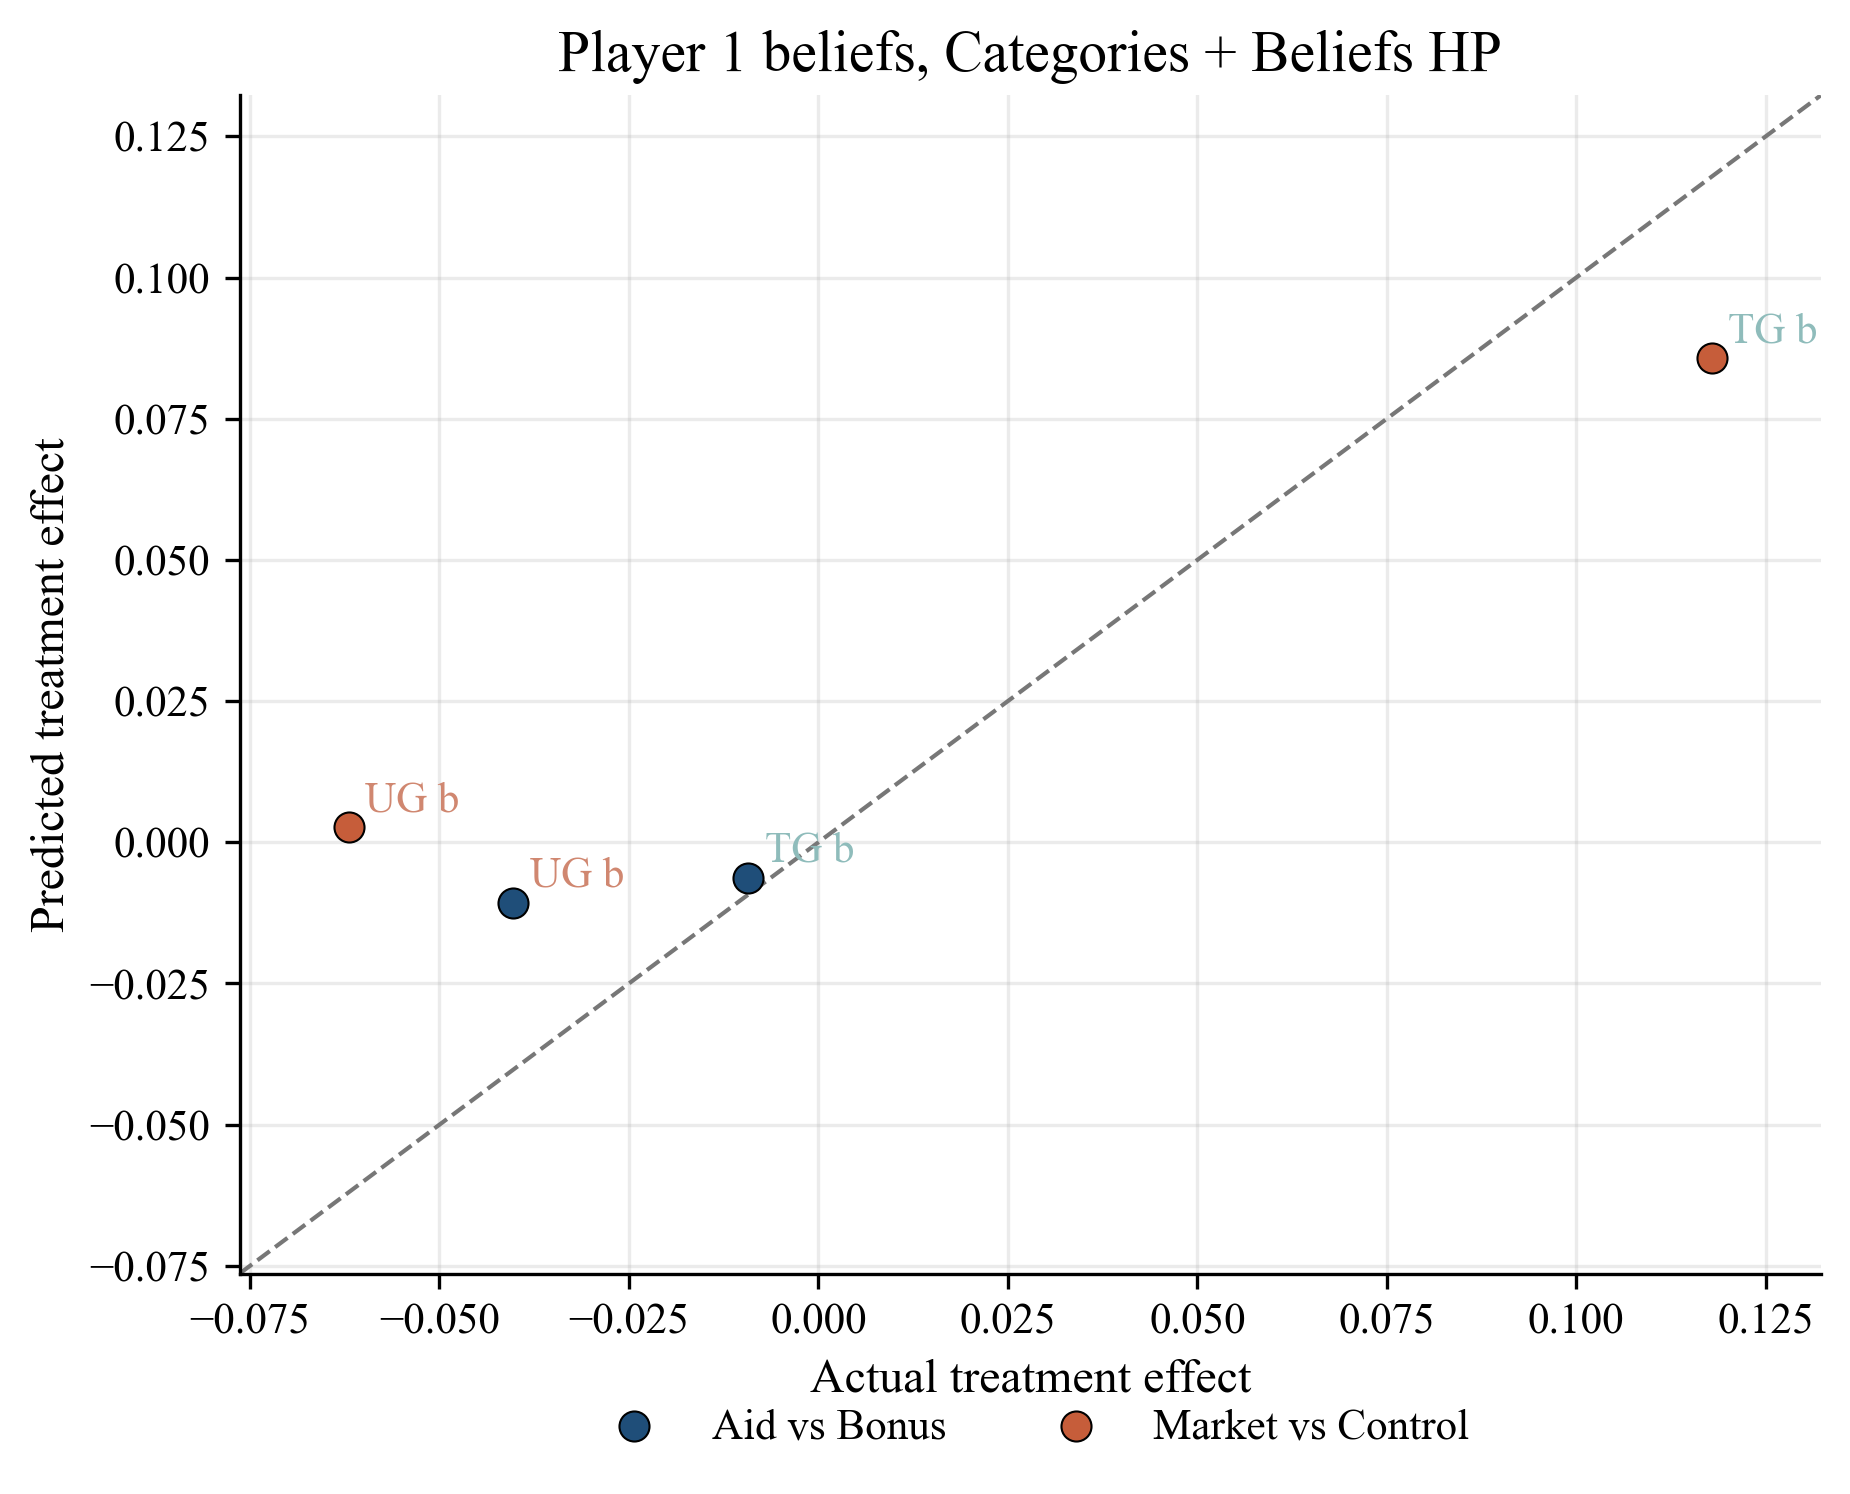
\includegraphics[width=0.74\textwidth]{cats_hp_instability_p1_beliefs.png}
\caption{Predicted vs actual treatment effects for Player 1 chosen-action beliefs, Categories + Beliefs specification. Each point is an outcome-by-comparison cell; the 45-degree line marks exact fit.}
\label{fig:instability_p1_beliefs}
\end{figure}

\begin{figure}[!htbp]
\centering
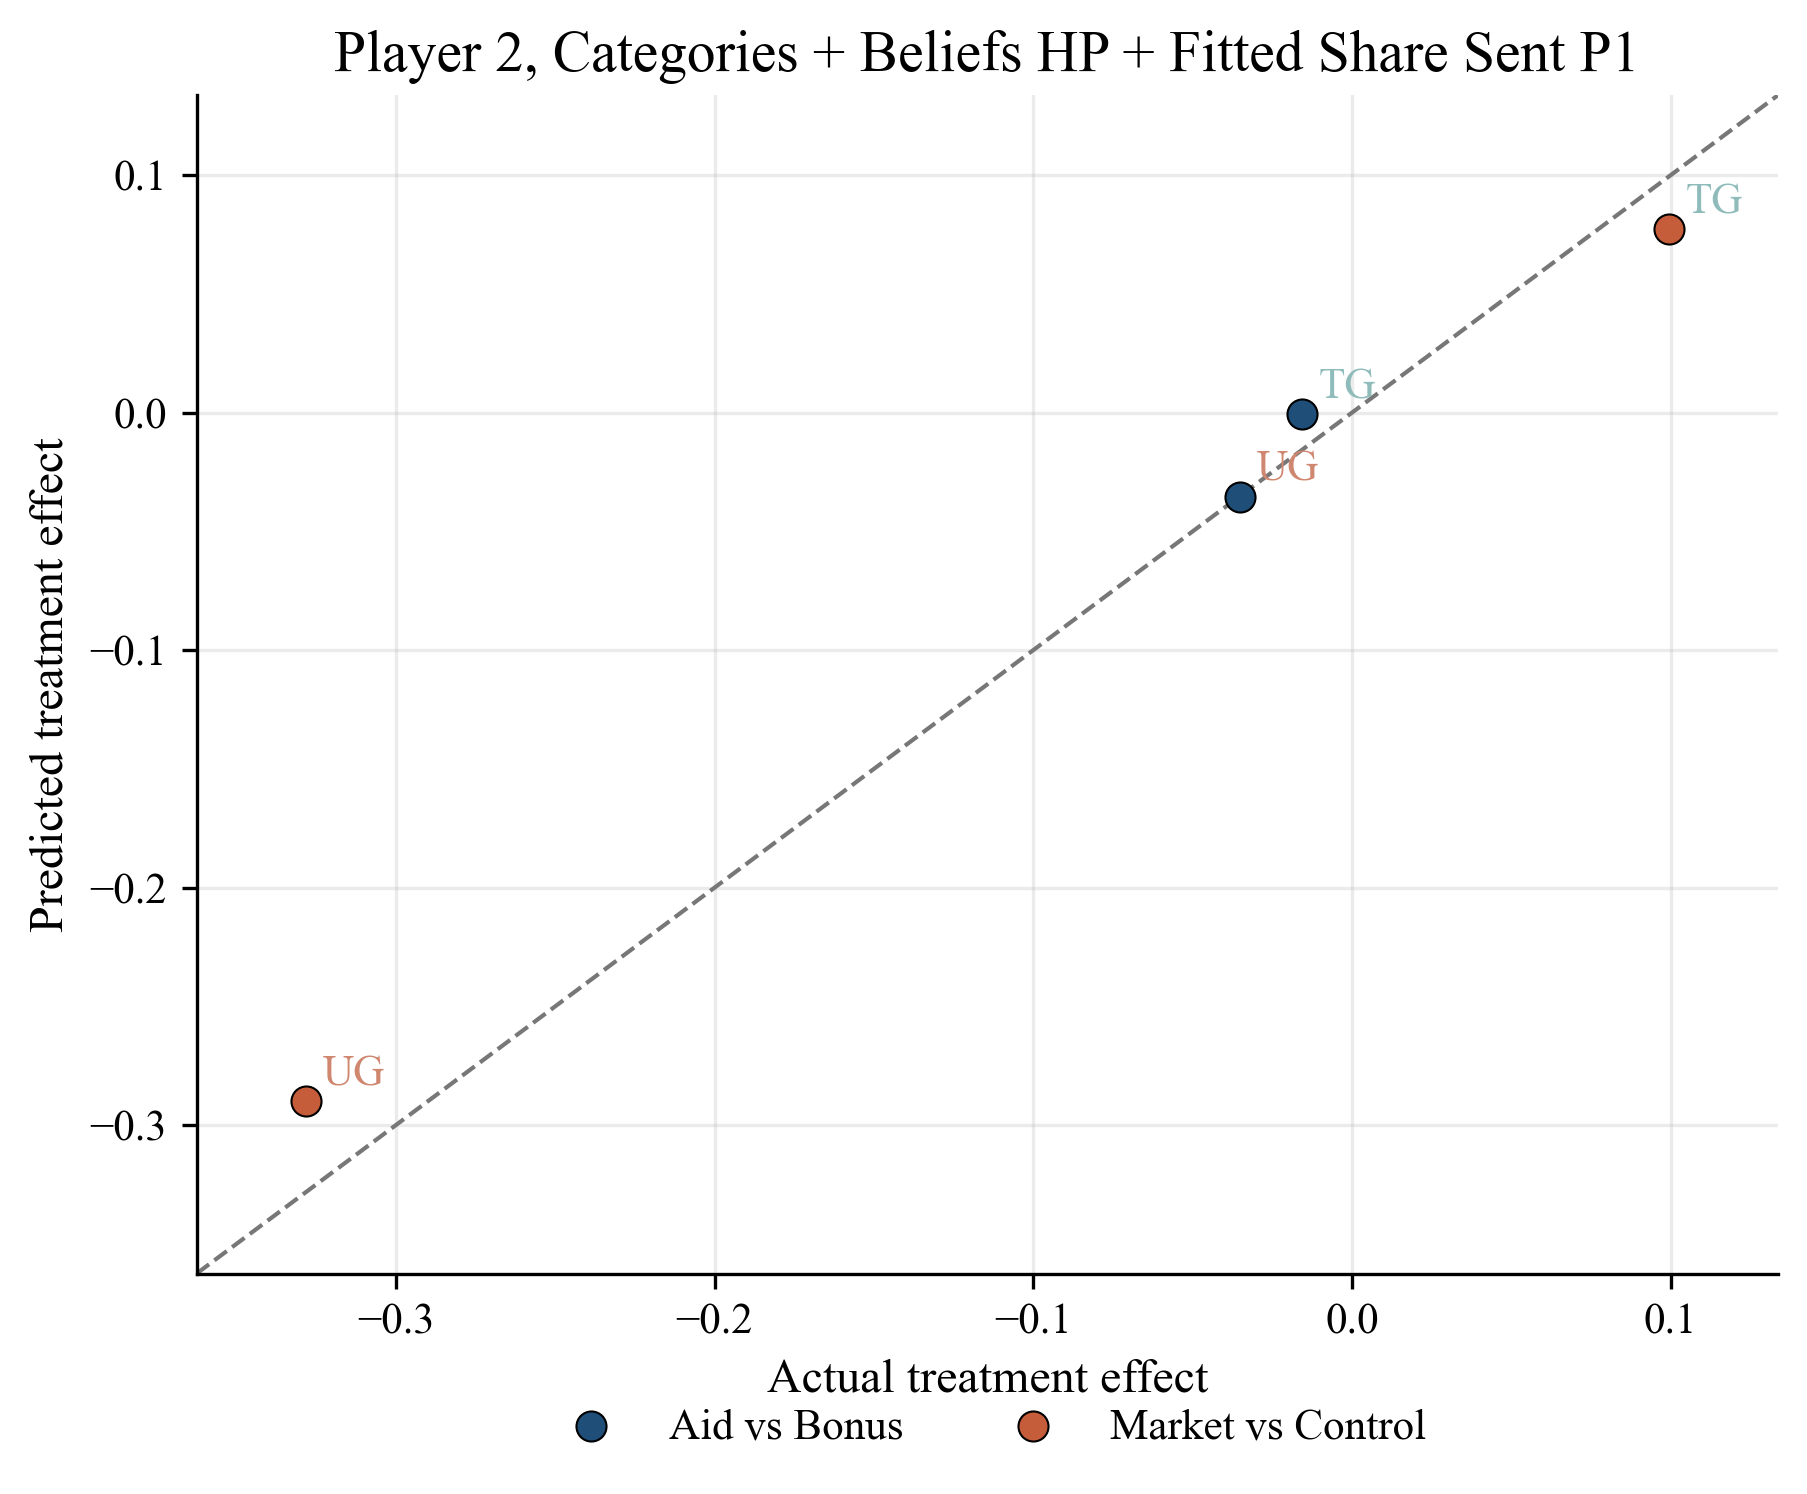
\includegraphics[width=0.74\textwidth]{cats_hp_instability_p2.png}
\caption{Predicted vs actual treatment effects for Player 2 outcomes, Categories + Beliefs specification with fitted Player 1 action. Each point is an outcome-by-comparison cell; the 45-degree line marks exact fit.}
\label{fig:instability_p2}
\end{figure}

\begin{figure}[!htbp]
\centering
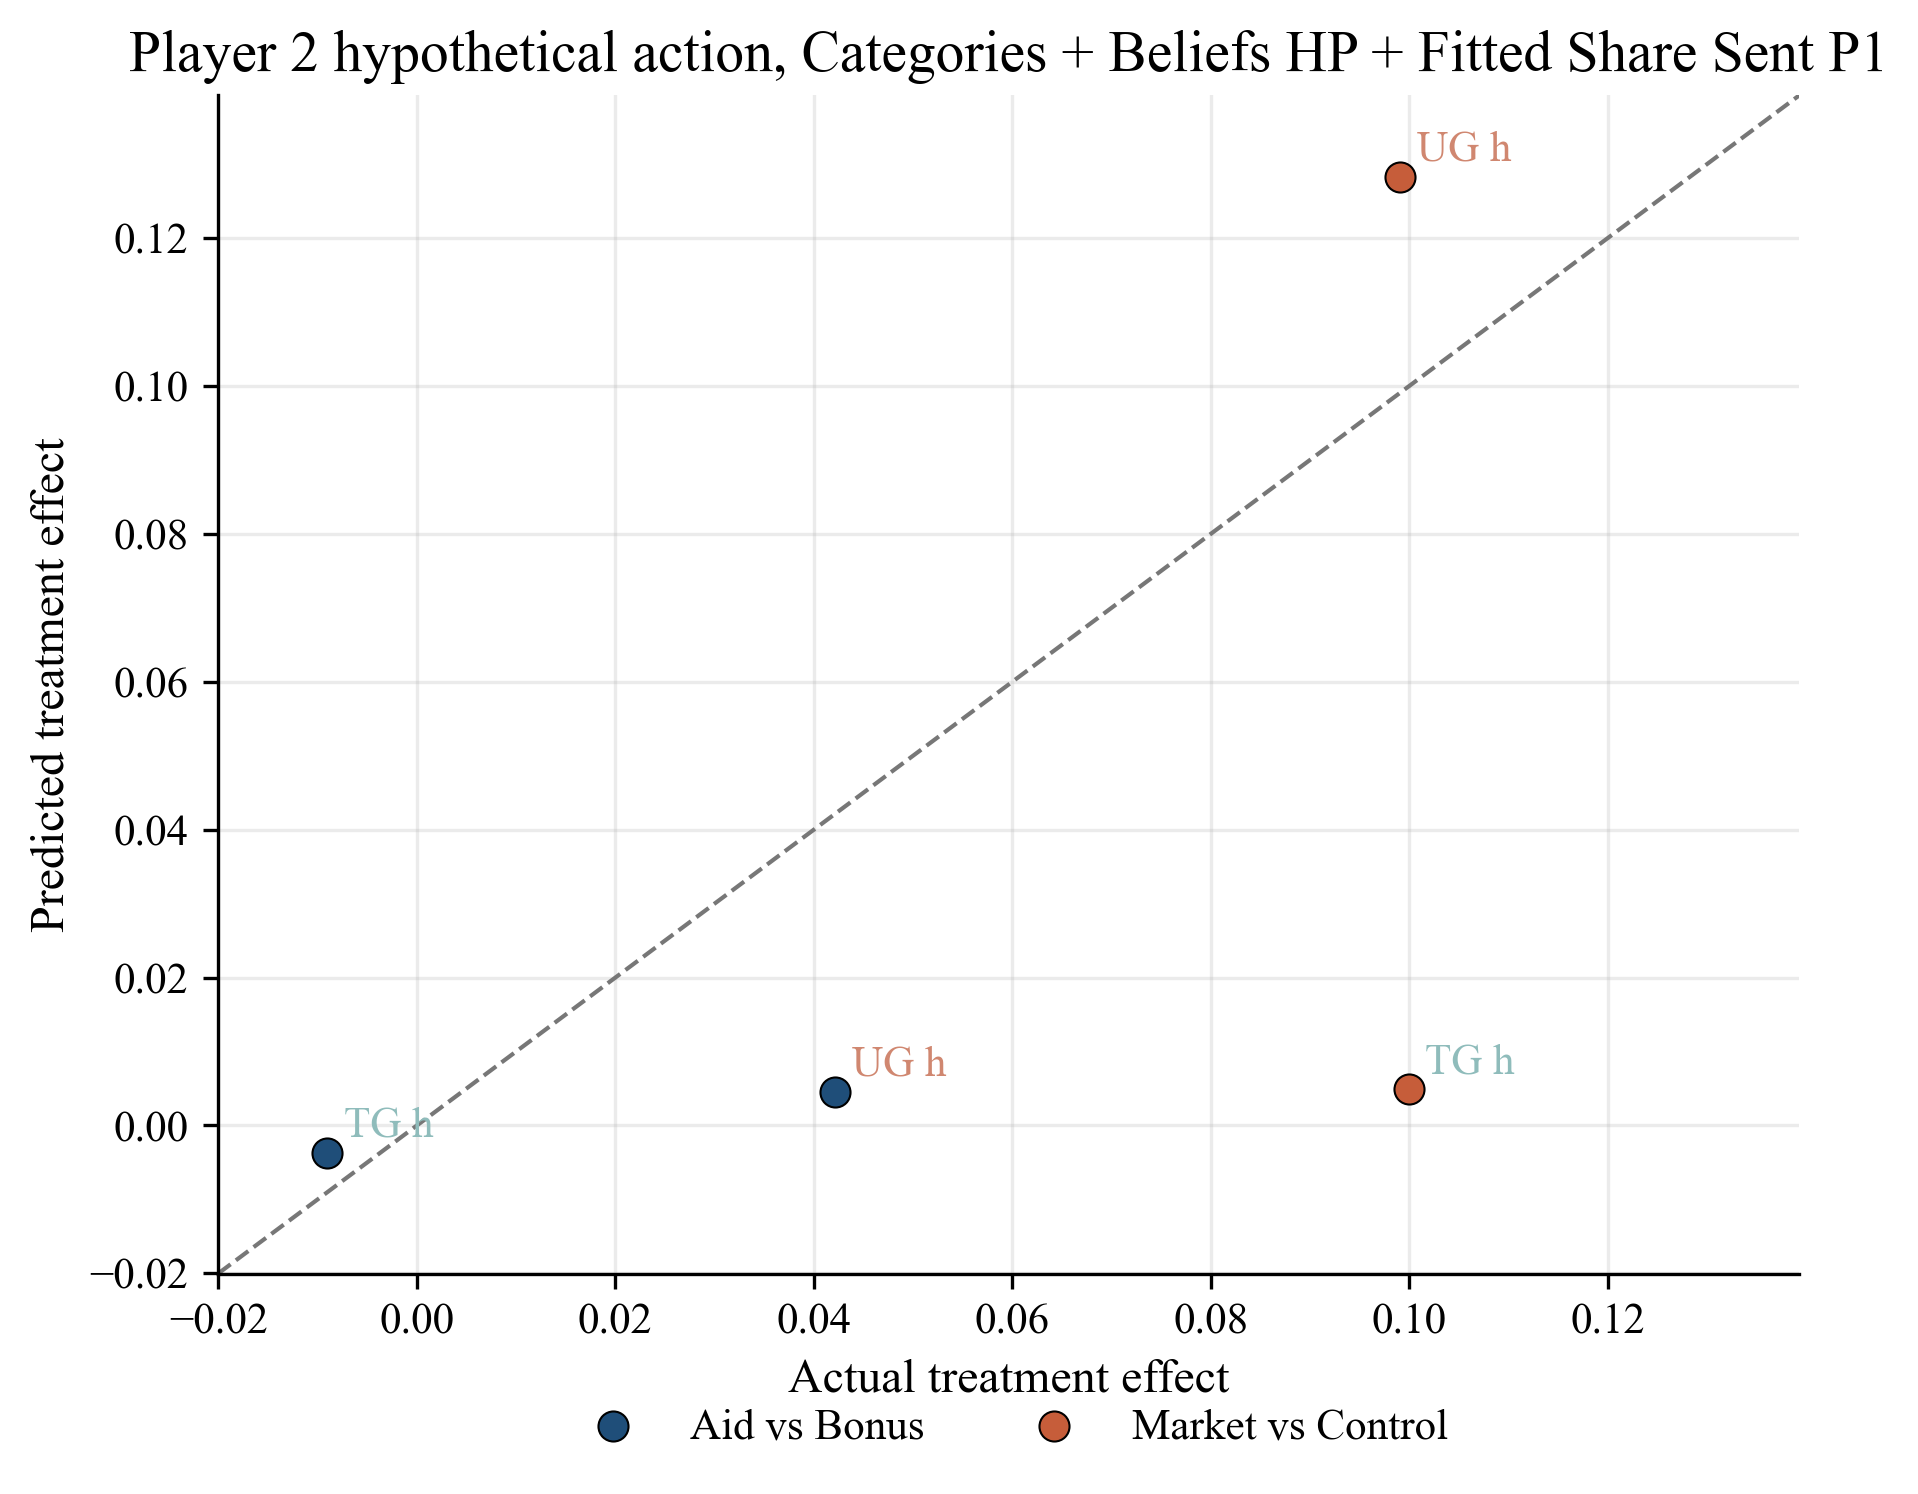
\includegraphics[width=0.74\textwidth]{cats_hp_instability_p2_hyp.png}
\caption{Predicted vs actual treatment effects for Player 2 hypothetical actions, Categories + Beliefs specification with fitted Player 1 action. Each point is an outcome-by-comparison cell; the 45-degree line marks exact fit.}
\label{fig:instability_p2_hyp}
\end{figure}

\begin{table}[!htbp]
\centering
\caption{\textbf{Instability calibration regressions, Categories + Beliefs HP}}
\label{tab:cats_hp_instability_regs}
\begin{tabular}{lccc}
\toprule
& All & Player 1 & Player 2 \\
\midrule
Intercept & -0.005 & -0.016* & 0.010 \\
& (0.010) & (0.008) & (0.016) \\
Predicted & 1.238*** & 1.771*** & 1.100*** \\
& (0.119) & (0.140) & (0.137) \\
Observations & 18 & 10 & 8 \\
$R^2$ & 0.871 & 0.952 & 0.915 \\
\bottomrule
\end{tabular}

\vspace{0.2cm}
\begin{minipage}{0.9\textwidth}
\footnotesize Notes: Unit of observation is an outcome-by-comparison cell from the fitted-values exercise. Each column reports the regression of the actual treatment effect on the predicted treatment effect. Standard errors in parentheses. $^*$ $p<0.1$, $^{**}$ $p<0.05$, $^{***}$ $p<0.01$.
\end{minipage}
\end{table}


The economic content of this exercise is the paper's central claim: the same handful of measured representations that distinguish who gives, offers, trusts, and rejects \emph{within} a context also account for how behavior moves \emph{across} contexts. The same categories therefore organize both variation across participants within a given context and behavioral change when the context changes.

% RESOLVED 2026-07-13 (was: TODO, NG open question i): receiver analysis = hypothetical actions in the main text (moved to the head of this subsection, before the regressions), category shifts and detail in Appendix app:player2, foundations in Appendix app:receiver.

\paragraph{From mean effects to heterogeneity.} The model's first implication in Section~\ref{sec:determination} is about dispersion, not means: within a treatment, behavior is heterogeneous because representations are, and a treatment that shifts the category mixture should reshape the whole outcome distribution, not just its center. Two statistics tie heterogeneity to representations directly: the share of within-treatment outcome variance that lies \emph{between} representation categories, by game and treatment; and the change in outcome dispersion that the shifted category mixture predicts, compared with the actual change.
Table~\ref{tab:heterogeneity_decomposition} reports the decomposition. In control, the between-category share of action variance is 0.66 in the DG-KW against 0.11 in the UG and 0.20 in the TG\@: where nothing disciplines the dictator, which representation a participant holds is most of the story, while rejection risk compresses offers toward the common standard so strongly that categories have little variance left to explain---the variance-domain counterpart of the mean compression of Section~\ref{sec:control}, and of Proposition~\ref{prop:ug}. The treatments move the sorting itself: under the market frame the DG-KW between-share collapses from 0.66 to 0.14 while overall dispersion widens (the standard deviation rises from 0.20 to 0.26). The frame does not merely reshuffle participants across categories that go on sorting behavior as before; it also moves behavior within categories---the sender-side counterpart of the within-category margin that the receiver decomposition of Appendix~\ref{app:receiver} makes explicit.

\begin{table}[!htbp]
\centering
\small
\renewcommand{\arraystretch}{1.15}
\caption{\textbf{Heterogeneity Tied to Representations: Variance Decomposition}}
\label{tab:heterogeneity_decomposition}
\begin{tabular}{ll rrr}
\toprule
Game & Condition & $N$ & SD of action & Between-category share \\
\midrule
DG-KW & Control & 399 & 0.204 & 0.663 \\
 & Market & 329 & 0.263 & 0.136 \\
 & Bonus & 390 & 0.171 & 0.613 \\
 & Aid & 400 & 0.197 & 0.584 \\
DG-LT & Control & 389 & 0.175 & 0.492 \\
 & Market & 347 & 0.178 & 0.109 \\
 & Bonus & 387 & 0.166 & 0.407 \\
 & Aid & 387 & 0.194 & 0.481 \\
UG & Control & 582 & 0.111 & 0.109 \\
 & Market & 501 & 0.260 & 0.061 \\
 & Bonus & 587 & 0.090 & 0.097 \\
 & Aid & 588 & 0.138 & 0.226 \\
TG & Control & 584 & 0.282 & 0.202 \\
 & Market & 563 & 0.285 & 0.250 \\
 & Bonus & 589 & 0.289 & 0.296 \\
 & Aid & 588 & 0.295 & 0.314 \\
\bottomrule
\end{tabular}
\begin{flushleft}
\footnotesize Notes: Player 1, classified responses only. ``Between-category share'' is the share of the within-condition variance of the action lying between the three representation categories (the $R^2$ of the action on category dummies).
\end{flushleft}
\end{table}


Table~\ref{tab:heterogeneity_predicted_actual} takes the accounting to dispersion. Reweighting the category-conditional action distributions by each arm's measured category shares---holding within-category behavior fixed---predicts the change in the standard deviation of behavior with the correct sign in all eight game-by-comparison cells. Magnitudes are close in the story comparisons of the two dictator games and understated where dispersion moves most (the UG story arms, and the DG-KW and UG under the market frame); the small actual changes in the remaining cells are matched only loosely. The table's mean columns show the same attenuation as Figures~\ref{fig:instability_p1}--\ref{fig:instability_p2_hyp} (predicted-to-actual ratios of 0.28--0.46 for the large market effects). The pattern is one message read twice: composition measured from text carries the direction in which every treatment reshapes both the level and the spread of behavior, and the market frame's residual is the within-category movement that composition alone cannot carry.
% INSERTED 2026-07-16 (SN decision, AA-reproduction gate lifted): E3 tables from 05; numbers audited against output/tables/paper_v2_new_stats.txt and the table files this session (between-shares 0.663/0.109/0.202 control, 0.136 DG-KW market; SD 0.204->0.263; dSD signs 8/8; mean ratios market 0.45/0.46/0.35/0.28).

\begin{table}[!htbp]
\centering
\small
\renewcommand{\arraystretch}{1.15}
\caption{\textbf{Predicted versus Actual Treatment Effects on Dispersion}}
\label{tab:heterogeneity_predicted_actual}
\begin{tabular}{ll rr rr}
\toprule
 & & \multicolumn{2}{c}{$\Delta$ Mean (pp)} & \multicolumn{2}{c}{$\Delta$ SD} \\
\cmidrule(lr){3-4}\cmidrule(lr){5-6}
Comparison & Game & Predicted & Actual & Predicted & Actual \\
\midrule
Aid vs Bonus & DG-KW & -3.9 & -5.9 & +0.022 & +0.026 \\
 & DG-LT & -4.0 & -5.0 & +0.023 & +0.028 \\
 & UG & -1.3 & -2.4 & +0.017 & +0.048 \\
 & TG & +0.3 & +0.8 & +0.001 & +0.005 \\
\midrule
Market vs Control & DG-KW & -4.5 & -10.1 & +0.019 & +0.059 \\
 & DG-LT & -9.9 & -21.5 & +0.010 & +0.003 \\
 & UG & -7.3 & -21.0 & +0.043 & +0.149 \\
 & TG & +4.2 & +15.0 & +0.019 & +0.003 \\
\bottomrule
\end{tabular}
\begin{flushleft}
\footnotesize Notes: Player 1, classified responses only. Predicted values reweight the category-conditional action distributions (means and variances pooled across the two conditions of each comparison) by each condition's category shares; the predicted effect is the mixture implication of the representation shift alone. Actual values are the raw between-condition differences.
\end{flushleft}
\end{table}


\paragraph{Surplus and inequality.}
\label{sec:surplus}

The market frame has opposite allocative consequences in the two strategic games: it destroys surplus in the UG and creates it in the TG\@. Table~\ref{tab:surplus_by_treatment} reports realized surplus by treatment (the DG is omitted because its total is fixed by design). In the UG, lower offers meet receivers who---despite representing the game less morally---still reject them often enough that acceptance falls from 94.7\% to 61.8\%, and expected surplus per pair falls from \$11.36 to \$7.42, roughly a third of the pie. In the TG, sends rise and realized surplus increases from \$11.81 to \$13.55 (a 15\% expansion; the maximum feasible surplus is \$18). The aid story has a small negative effect on UG surplus and none in the TG\@. The same contextual manipulation thus destroys surplus in a division problem and creates it in a production problem---a distinction invisible to any account in which ``market framing'' uniformly promotes or degrades prosociality. The forecast errors of Section~\ref{sec:forecast} are the mechanism: under the market frame, proposers expect brokers to accept low prices more readily than brokers actually do.

\begin{table}[!htbp]
\centering
\caption{\textbf{Treatment Effects on Realized Surplus}}
\label{tab:surplus_by_treatment}
\begin{tabular}{lcccccc}
\toprule
 & Control & Market & Market $-$ Control & Bonus & Aid & Aid $-$ Bonus \\
\midrule
UG: acceptance rate & 0.947 & 0.618 & -0.328$^{***}$ & 0.947 & 0.912 & -0.035$^{**}$ \\ % chktex 13
UG: expected surplus (\$) & 11.36 & 7.42 & -3.94$^{***}$ & 11.36 & 10.94 & -0.42$^{**}$ \\ % chktex 13
TG: realized surplus (\$) & 11.81 & 13.55 & 1.74$^{***}$ & 12.13 & 12.20 & 0.07 \\ % chktex 13
\bottomrule
\end{tabular}
\begin{flushleft}
\footnotesize Notes: In the Ultimatum Game, realized surplus per matched pair is \$12 if the receiver accepts and \$0 otherwise; the acceptance rate is computed over receivers responding to their matched sender's offer. In the Trust Game, realized surplus is $6+12s$ dollars, where $s$ is the sender's share sent; the receiver's return does not change total surplus. The Dictator Game is omitted because total surplus is fixed at \$12 by design. Differences are tested with Welch two-sample $t$-tests. $^{*}p<0.10$, $^{**}p<0.05$, $^{***}p<0.01$.
\end{flushleft}
\end{table}



\subsection{Circling Back: The Two Dictator Games}
\label{sec:kwlt}

Return to Figure~\ref{fig:intro_kw_lt}. Under the representations account, DG-KW and DG-LT differ not in what participants can do but in what the situation evokes: a windfall to be shared versus an allocation already in place, where taking from another's pile is theft. The evidence bears this out. Applying the pre-registered representation measures to the two games (Appendix~\ref{app:hp}) shows that they evoke different counterparts and different moral situations: taking-type categories that are virtually absent in DG-KW appear in DG-LT (Theft: 0.5\% vs 4.0\% of responses), and a symmetrized decomposition attributes about half of the roughly \$1 gap in mean allocations in the hypothetical-allocation sample to differences in the \emph{distribution} of representations, with the remainder coming from behavior conditional on the representation (Table~\ref{tab:decomposition_sym_kw_lt}).

The treatments put the gap on a common scale. The KW--LT difference in mean transfers---6.4 points of the budget---is of the same order as the Aid--Bonus effect on dictator giving (5.6 points) and smaller than the market effect (10.9 points): two payoff-equivalent descriptions of the \emph{same} dictator game move behavior about as much as reading a different story, and less than embedding the game in a market.\footnote{With 95\% confidence intervals, in percentage points of the budget: LT $-$ KW $+6.4$ $[+3.8,\,+8.9]$ (bootstrap, 5{,}000 draws); Aid $-$ Bonus $-5.6$ $[-8.2,\,-3.0]$ and Market $-$ Control $-10.9$ $[-14.1,\,-7.7]$ (Welch intervals).}
% VERIFIED 2026-07-09 via 05 (output/tables/kwlt_treatment_scale.tex); CIs inserted as the footnote 2026-07-16 (SN decision, AA gate lifted) --- the three-row table itself deliberately stays out of the paper (the claim is qualitative; CIs suffice).
The within-subject arms sharpen the point at the individual level (Appendix~\ref{app:within}): when the same participant plays both games, 46\% change their choice, and choice switching is tightly linked to representation switching---80\% of those whose category changes across the two games change their choice, against 36\% of those whose category is stable. When the frame switches from abstract to market with the game fixed, 73--82\% change their choice and over half change their representation category. To first order, behavioral instability tracks representational instability---across frames, across stories, and within the person.

\section{Conclusions}
\label{sec:discussion}

Strategic behavior is shaped by context; on the account this paper develops and tests, representations are the channel. Identical rules evoke different situations depending on strategic structure and on payoff-irrelevant cues; the evoked situation directs attention across own earnings, total surplus, and the sharing norm, and supplies the counterpart one imagines facing; attention and beliefs together shape actions. On this account, within-context heterogeneity and cross-context instability are the same phenomenon: people differ in the situations a game evokes for them, and contexts differ in the situations they evoke on average.

Could stable preferences plus correct beliefs explain our treatment effects, with context operating through equilibrium expectations---for instance, the market frame signaling that others will behave selfishly, and best responses adjusting? The forecast-error evidence of Section~\ref{sec:forecast} says no. In the UG, beliefs overshoot behavior under the market frame and undershoot it elsewhere, while TG errors stay small; treatments move chosen-action errors by more than 25 percentage points, and the selection-immune reference-action errors move in the same direction, if by less. Beliefs look like outputs of the representation---a proposer who sees a market expects market-like acceptance, a sender who sees a joint venture expects reciprocation---rather than like calibrated forecasts of a treatment-shifted opponent. This also cautions against interpreting elicited beliefs in games as measures of information: two participants facing the same distribution of opponents can hold different beliefs because they represent the game differently.

Experimenter demand is the other cross-cutting candidate. Three features of the design resist it. The same manipulation moves behavior in opposite directions across games, so a compliant participant would need to divine that the experimenter ``wants'' lower ultimatum offers but higher trust-game sends from the same market frame. The stories never mention the game, and their effects fall with the measured structural distance between story and game rather than following the stories' surface moral content---the charitable story \emph{reduces} giving. And the open-ended answers, written after an unincentivized prompt, predict incentivized beliefs about the other player and hypothetical responses at fixed reference actions, which telling the experimenter what she wants to hear does not produce. Formal bounding exercises are available \citep{deQuidtHaushoferRoth2018}; the sign-reversal pattern alone places tight limits on the demand channel.
% INSERTED 2026-07-16 (from coauthor_discussion_drafts.md section 1, account 5 --- the one alternative account the paper did not yet address; SN approved).

Two substantive lessons follow. First, social context need not mechanically produce generous behavior. Relative to a workplace-bonus story, the aid story shifted reported reasoning toward self-interest and reduced dictator transfers and ultimatum offers. Because the stories differ jointly in focal characters, entitlement, need, and the explicit case for sharing, this comparison does not isolate the effects of charity or hardship per se. It shows instead that a narrative with charitable content need not increase sharing relative to an alternative narrative that foregrounds contribution and reciprocity. Interventions that rely on context to encourage prosociality may therefore have unintended effects when they change what the situation appears to be about. Second, market framing crowds out moral reasoning but can foster cooperation. The market frame crowded out moral representations in every game, echoing longstanding concerns about markets and morals \citep{FalkSzech2013, GneezyRustichini2000}; but in the trust game the very same frame raised trust, repayment expectations, and surplus (Section~\ref{sec:ge}), consistent with the ethics of sharing being replaced by the logic of mutually beneficial exchange. Whether a market cue degrades or improves outcomes depends on whether the underlying interaction is a division or a joint production problem.

The representation lens also speaks to game theory beyond our three games. If representations rather than game forms are the objects players best-respond to, then learning to play a game---the prisoner's dilemma, a public goods game---is learning a \emph{shared} representation, and stability is representational: occasional deviations can be destabilizing not because they change payoffs but because they change what the situation appears to be. Repeated play under a stable context may work precisely by fading the naturalistic frame and creating a context of its own. And the salience that makes focal points focal \citep{Schelling1960} is, in this language, a property of the representations a description evokes rather than of the game form---a reading consistent with the predictable effects of visual salience on strategic choice documented by \citet{LiCamerer2022}.
% TODO (NG): develop this paragraph for the call --- learning in PD/public-goods games, instability upon occasional deviations, the repeated game as a self-generated context. RESOLVED 2026-07-16 (SN: "it must be the one we identified"): the Camerer QJE = Li & Camerer (2022, QJE 137(3), 1849-1900), verified and cited above; NG can swap if he meant another. Schelling1960 verified present in references.bib.
% RESOLVED 2026-07-16 (was NG open question ii, SP placement): SP narrative implemented per NG's 07-11 decision --- control SP in Section 3.2 (categories -> SP -> giving), market anonymity + generalized trust with verified citations in Section 4.2; the "here vs 5.1" question is superseded.

The measurement strategy developed here---eliciting open-ended reasoning at scale and classifying it into representation categories, now paired with direct measurement of the beliefs inside the representation---is portable: to bargaining and labor-market experiments where entitlements and frames are known to matter \citep{HoffmanMcCabeShachatSmith1994, KahnemanKnetschThaler1986}, to field settings where the same transaction is embedded in different relationships, and to the study of how experience reshapes the categories themselves \citep{BordaloGennaioliShleifer2020, BordaloConlonGennaioliKwonShleifer2026}. What determines which representation a context evokes for whom---and how policy can move representations deliberately---strikes us as the central open question.

\bibliographystyle{plainnat}
\bibliography{references}

\clearpage
\appendix

\section{Proofs of Propositions}
\label{app:proofs}

Throughout, attention weights are strictly positive, $\rho,\sigma,\mu>0$, and in the ultimatum game $a,b>0$. Each objective below is strictly concave and differentiable on $[0,1]$, so the constrained maximizer is unique and equals the unconstrained solution projected onto $[0,1]$ (the censoring in the propositions); comparative statics are stated at interior optima, where the projection is the identity.

\begin{proof}[Proof of Proposition~\ref{prop:dg}]
With $W(t)=1$ and $\pi_R=t$, the objective is $u(t)=\rho-\sigma t-\frac{\mu}{2}\left(t-\frac12\right)^{2}$, which is strictly concave ($u''=-\mu<0$). The first-order condition $-\sigma-\mu\left(t-\frac12\right)=0$ gives $t^{\ast}=\frac12-\sigma/\mu$. Since $\sigma/\mu>0$, $t^{\ast}<\frac12$, so the upper bound never binds and $t^{DG}=\max\{0,\,t^{\ast}\}<\frac12$. The solution is strictly decreasing in $\sigma/\mu$ where interior and constant at zero for $\sigma/\mu\ge\frac12$; $\rho$ enters the objective only through the additive constant $\rho\,W(t)=\rho$, so it leaves the maximizer unchanged.
\end{proof}

\begin{proof}[Proof of Proposition~\ref{prop:ug}]
The objective $v(t)=(a+bt)(\rho-\sigma t)-\frac{\mu}{2}\left(t-\frac12\right)^{2}$ has $v'(t)=b\rho-a\sigma-2b\sigma t-\mu\left(t-\frac12\right)$ and $v''(t)=-(2b\sigma+\mu)<0$: $v$ is strictly concave. The first-order condition gives $t\,(2b\sigma+\mu)=b\rho-a\sigma+\frac{\mu}{2}$, and subtracting $\frac12$ from the resulting $t$ yields~\eqref{eq:ug_offer}. The censored solution lies in $(0,1)$ if and only if $\bigl|b\rho-(a+b)\,\sigma\bigr|<b\sigma+\mu/2$, half the curvature $2b\sigma+\mu$.

(i) If $t^{DG}=0$, interiority gives $t^{UG}>0=t^{DG}$. If $t^{DG}=\frac12-\sigma/\mu>0$, putting the difference over the common denominator $\mu\,(2b\sigma+\mu)$ gives
\begin{equation*}
t^{UG}-t^{DG}\;=\;\frac{b\rho-(a+b)\,\sigma}{2b\sigma+\mu}+\frac{\sigma}{\mu}\;=\;\frac{\mu b\rho+2b\sigma^{2}+\mu\sigma\,(1-a-b)}{\mu\,(2b\sigma+\mu)},
\end{equation*}
and $a+b\le 1$ makes every term in the numerator non-negative, with $\mu b\rho>0$; hence $t^{UG}>t^{DG}$.

(ii) Differentiating~\eqref{eq:ug_offer},
\begin{equation*}
\frac{\partial t^{UG}}{\partial \rho}=\frac{b}{2b\sigma+\mu}>0,\qquad
\frac{\partial t^{UG}}{\partial \sigma}=-\,\frac{(a+b)\,\mu+2b^{2}\rho}{(2b\sigma+\mu)^{2}}<0,\qquad
\frac{\partial t^{UG}}{\partial \mu}=-\,\frac{t^{UG}-\tfrac12}{2b\sigma+\mu},
\end{equation*}
where the middle expression follows from the quotient rule and is negative unconditionally and the last expression is positive when $t^{UG}<\frac12$ and negative when $t^{UG}>\frac12$: the norm weight pulls the offer toward the equal split.

(iii) Only the numerator of the second term in~\eqref{eq:ug_offer} depends on $a$, so $\partial t^{UG}/\partial a=-\sigma/(2b\sigma+\mu)<0$. The sensitivity $\sigma/(2b\sigma+\mu)$ has derivative $\mu/(2b\sigma+\mu)^{2}>0$ in $\sigma$ and $-\sigma/(2b\sigma+\mu)^{2}<0$ in $\mu$.
\end{proof}

\begin{proof}[Proof of Proposition~\ref{prop:tg}]
The objective $w(t)=\rho\,(1+rt)-\sigma(1+r)(1-s)\,t-\frac{\mu}{2}\left(t-\frac12\right)^{2}$ has $w'(t)=\rho r-\sigma(1+r)(1-s)-\mu\left(t-\frac12\right)$ and $w''(t)=-\mu<0$, so the first-order condition gives~\eqref{eq:tg_send}. The censored solution lies in $(0,1)$ if and only if $\bigl|\rho r-\sigma(1+r)(1-s)\bigr|<\mu/2$. At an interior optimum,
\begin{equation*}
\frac{\partial t^{TG}}{\partial \rho}=\frac{r}{\mu}>0,\qquad
\frac{\partial t^{TG}}{\partial s}=\frac{\sigma(1+r)}{\mu}>0,\qquad
\frac{\partial t^{TG}}{\partial \sigma}=-\,\frac{(1+r)(1-s)}{\mu}<0,
\end{equation*}
and $\partial t^{TG}/\partial\mu=-\bigl[\rho r-\sigma(1+r)(1-s)\bigr]/\mu^{2}=-\bigl(t^{TG}-\tfrac12\bigr)/\mu$: the norm weight pulls the send toward the equal split. As $\mu\to 0$ the objective converges to the affine function $\rho+\bigl[\rho r-\sigma(1+r)(1-s)\bigr]\,t$, whose maximizer is $t=1$ if the slope is positive and $t=0$ if it is negative. For a purely material sender, $\rho=\sigma$, the objective reduces to $\sigma\,\pi_S$ with $\pi_S=1+t\,\bigl[s(1+r)-1\bigr]$, so the slope is $\sigma\bigl[s(1+r)-1\bigr]$: she sends everything if $s(1+r)>1$ and nothing if $s(1+r)<1$. Finally, if $t^{DG}=0$, interiority gives $t^{TG}>0=t^{DG}$; if $t^{DG}=\frac12-\sigma/\mu$, then
\begin{equation*}
t^{TG}-t^{DG}\;=\;\frac{\rho r-\sigma(1+r)(1-s)+\sigma}{\mu}\;=\;\frac{r\,\bigl[\rho-\sigma(1-s)\bigr]+\sigma s}{\mu},
\end{equation*}
a sum of two non-negative terms when $\rho\ge\sigma(1-s)$, both zero only if $s=0$ and $\rho=\sigma$---the sender who expects nothing back and puts no weight on the surplus, for whom the material pull of sending, $\rho r-\sigma(1+r)=-\sigma$, is exactly the dictator's.
\end{proof}

\begin{proof}[Proof of Proposition~\ref{prop:welfare}]
Welfare statements follow from the chain rule $\partial V_g/\partial\theta=W_g'\cdot\partial t^{g}/\partial\theta$, where the pie's sensitivity to the action is $W_{UG}'=p'(t)=b$ (expected pie $p(t)\cdot 1$) and $W_{TG}'=r$, combined with the action derivatives in the proofs of Propositions~\ref{prop:ug} and~\ref{prop:tg}: for (i), $\partial V_{UG}/\partial\rho=b\cdot b/(2b\sigma+\mu)$ and $\partial V_{TG}/\partial\rho=r\cdot r/\mu$; for (ii), $\partial V_{UG}/\partial\sigma=b\cdot\partial t^{UG}/\partial\sigma<0$ and $\partial V_{TG}/\partial\sigma=r\cdot\partial t^{TG}/\partial\sigma<0$; for (iii), $\partial V_g/\partial\mu=W_g'\cdot\partial t^{g}/\partial\mu$, and both games have $\partial t^{g}/\partial\mu$ proportional to $-(t^{g}-\tfrac12)$; for (iv), $\partial V_{UG}/\partial a=1+b\cdot\partial t^{UG}/\partial a=1-b\sigma/(2b\sigma+\mu)$ and $\partial V_{TG}/\partial s=r\cdot\sigma(1+r)/\mu$. The counterpart's expected payoff: in the ultimatum game $\partial\bigl[p(t)t\bigr]/\partial\sigma=\bigl(bt+p(t)\bigr)\,\partial t^{UG}/\partial\sigma<0$; in the trust game $\partial\bigl[(1-s_a)(1+r)t\bigr]/\partial\sigma=(1-s_a)(1+r)\,\partial t^{TG}/\partial\sigma<0$. The sender's own expected payoff: $\partial\bigl[p(t)(1-t)\bigr]/\partial\sigma=\bigl[b(1-t^{UG})-p(t^{UG})\bigr]\,\partial t^{UG}/\partial\sigma$, and $b(1-t)-p(t)=b(1-2t)-a$, so with $\partial t^{UG}/\partial\sigma<0$ the sender's own expected payoff falls precisely when $b(1-2t^{UG})>a$; a witness: $a=1/20$, $b=3/5$, $\rho=1/10$, $\sigma=1$, $\mu=1$ gives the interior offer $t^{UG}=0.232$, $b(1-2t^{UG})=0.32>0.05=a$, and $\partial\bigl[p(t)(1-t)\bigr]/\partial\sigma=-0.04<0$.
\end{proof}

\begin{proof}[Proof of Remark~\ref{rem:realized}]
For an actual acceptance schedule $\hat p$ with $\hat p'>0$, the chain rule gives $\partial\hat V_{UG}/\partial\theta=\hat p'(t^{UG})\cdot\partial t^{UG}/\partial\theta$ for $\theta\in\{\rho,\sigma,\mu\}$, the same signs as in (i)--(iii), while $\partial\hat V_{UG}/\partial a=\hat p'(t^{UG})\cdot\partial t^{UG}/\partial a=-\hat p'\,\sigma/(2b\sigma+\mu)<0$, reversing (iv); in the trust game $\hat V_{TG}=1+r\,t^{TG}$ coincides with $V_{TG}$, so $\partial\hat V_{TG}/\partial s=r\sigma(1+r)/\mu>0$ is unchanged.
\end{proof}

\begin{proof}[Proof of Proposition~\ref{prop:inequality}]
Conditional on trade, $D_{DG}=1-2t^{DG}=2\sigma/\mu$ and $D_{UG}=1-2t^{UG}=2\bigl[(a+b)\sigma-b\rho\bigr]/(2b\sigma+\mu)$, whence $\partial D_{UG}/\partial\sigma=2\bigl[(a+b)\mu+2b^{2}\rho\bigr]/(2b\sigma+\mu)^{2}>0$, $\partial D_{UG}/\partial\rho=-2b/(2b\sigma+\mu)<0$, and $\partial D_{UG}/\partial\mu=-D_{UG}/(2b\sigma+\mu)$ by direct differentiation. In the trust game $D_{TG}=(1-t)+s_a(1+r)t-(1-s_a)(1+r)t=1-t\bigl[1+(1+r)(1-2s_a)\bigr]$, affine in $t$ with slope $-k$, $k\equiv1+(1+r)(1-2s_a)$, positive iff $s_a<(2+r)/\bigl(2(1+r)\bigr)$; since $\partial t^{TG}/\partial\mu=-(t^{TG}-\tfrac12)/\mu$, $\partial D_{TG}/\partial\mu=-\bigl(D_{TG}-D_{TG}(\tfrac12)\bigr)/\mu$ with $D_{TG}(\tfrac12)=1-k/2=\bigl[1-(1+r)(1-2s_a)\bigr]/2$, which is zero iff $s_a=r/\bigl(2(1+r)\bigr)$.
\end{proof}

\section{Endogenizing Second-Mover Behavior}
\label{app:receiver}
% Inserted 2026-07-13 per the AA+NG email thread (AA: p(t) and s stay primitives in the main text, endogenizations as appendix extensions; NG: "sarebbe ottimo avere in appendice una formalizzazione che ci permette di dire nel testo che queste funzioni possono essere endogeneizzate e dipendono da come il sender percepisce la rappresentazione del receiver"). Content mirrors model-2.tex: rem:foundation and rem:return moved here verbatim from Section 2; the closing paragraphs port the note's section "Receiver's Behavior" (retitled by SN 2026-07-13 from "Bringing the Receiver into the Picture"). 2026-07-13: rem:return split into the foundation Remark + Proposition prop:tg_endog (declining schedule; proof inline here, in the note's appendix there).

The main text treats the acceptance schedule $p(t)=a+bt$ and the returned share $s$ as primitives of the sender's representation. This appendix endogenizes them: both schedules arise from the receiver's own moral psychology, so what the sender holds as a belief is a representation of the \emph{receiver's motives}---of how the sender perceives the receiver's representation. It then closes the model by making the receiver a full player, with her own retrieval problem cued by the very action she faces.

\begin{remark}[Endogenous acceptance schedule]
\label{rem:foundation}
The linear acceptance schedule can be founded in a moral psychology similar to the one we introduced above for senders. Endow the receiver with attention weights $\hat{\boldsymbol{\alpha}}=(\hat\rho,\hat\sigma,\hat\mu)$. Assume that the idealistic principle is applied to the sender's action: the receiver suffers from the offer's inequity and feels this cost whether or not the offer is accepted. Moreover, assume that rejection delivers a psychological benefit of \emph{protest}, $\psi\ge 0$, which is drawn from a distribution $F$ and weighted by moral attention. In this case, the inequity-aversion term cancels from the accept--reject margin and the receiver accepts $t$ if and only if $\hat\rho-\hat\sigma(1-t)\ge\hat\mu\,\psi$, so the acceptance probability is $F\bigl[(\hat\rho-\hat\sigma+\hat\sigma t)/\hat\mu\bigr]$. For $\psi$ uniform on $[0,\bar\Psi]$ this is exactly $p(t)=a+bt$ with
\begin{equation*}
a=\frac{\hat\rho-\hat\sigma}{\hat\mu\bar\Psi},\qquad b=\frac{\hat\sigma}{\hat\mu\bar\Psi}.
\end{equation*}
The believed acceptance schedule $(a,b)$ is therefore a representation of the \emph{receiver's motives}: imagining a punitive receiver (high $\hat\mu\bar\Psi$---our \emph{Moral bad} category) scales acceptance down across the board, while imagining a self-interested receiver (high $\hat\sigma$) makes acceptance sensitive to money. Note also that $p(1)=a+b=\hat\rho/(\hat\mu\bar\Psi)$, so the condition $a+b\le 1$ in Proposition~\ref{prop:ug} has a natural reading: the imagined receiver's protest weight is large enough that even a full-split offer is not certain to be accepted.
\end{remark}

\begin{remark}[Endogenous return schedule]
\label{rem:return}
The believed return can be founded in the same moral psychology as the acceptance schedule of Remark~\ref{rem:foundation}. Endow the imagined receiver with attention weights $\hat{\boldsymbol{\alpha}}=(\hat\rho,\hat\sigma,\hat\mu)$. Holding the output $(1+r)t$, the receiver is a dictator over it: total wealth $1+rt$ is fixed no matter how much she returns, so $\hat\rho$ is idle and she trades own earnings against a norm of returning half of a target pie $X$, choosing the returned amount $y$ to maximize $\hat\rho(1+rt)-\hat\sigma(1-t+y)-\tfrac{\hat\mu}{2}\bigl(y/X-\tfrac12\bigr)^{2}$. The natural targets are the amount sent ($X=t$), the output ($X=(1+r)t$), and total wealth ($X=1+rt$), and for every target the optimal returned share of the target is the same expression, $y^{*}/X=\tfrac12-(\hat\sigma/\hat\mu)X$. Under the first two targets the believed returned share of the output is affine and \emph{decreasing} in the send---with the amount-sent target, $s(t)=\bigl[\tfrac12-(\hat\sigma/\hat\mu)t\bigr]/(1+r)$; with the output target, $s(t)=\tfrac12-(\hat\sigma/\hat\mu)(1+r)t$. Thus, the foundation has a testable signature: believed return shares should decline in the send, which the two elicited belief points per sender (reference and chosen action) can check. The total-wealth target is ill behaved---at small sends the norm target exceeds the pot itself, forcing full return below a threshold and a kinked schedule---so the amount-sent and output targets are the tractable specifications. As in Remark~\ref{rem:foundation}, the believed schedule is a representation of the receiver's motives, here through the imagined selfishness ratio $\hat\sigma/\hat\mu$.
\end{remark}

Replacing the constant share with the founded, declining schedule---or any affine one---leaves the trust-game analysis intact:

\begin{proposition}[Trust send with a declining return schedule]
\label{prop:tg_endog}
Under any affine believed schedule $s(t)=s_{0}-s_{1}t$ with $0\le s_{0}<1$ and $s_{1}\ge 0$, the sender's objective remains strictly concave, and the optimal send is
\begin{equation}
t^{TG}\;=\;\frac{\mu/2+\rho r-\sigma(1+r)(1-s_{0})}{\mu+2\sigma(1+r)s_{1}},
\label{eq:tg_send_endog}
\end{equation}
censored to $[0,1]$, which nests equation~\eqref{eq:tg_send} at $s_{1}=0$; the send is interior if and only if $\bigl|\rho r-\sigma(1+r)(1-s_{0}+s_{1})\bigr|<\mu/2+\sigma(1+r)s_{1}$. At an interior optimum: (i) the send is increasing in $\rho$, decreasing in $\sigma$, and moved toward the equal split by $\mu$, as in Proposition~\ref{prop:tg}; (ii) the send is increasing in the believed level $s_{0}$, with sensitivity $\sigma(1+r)/\bigl(\mu+2\sigma(1+r)s_{1}\bigr)$---damped by the believed slope exactly as the ultimatum sensitivity $\sigma/(2b\sigma+\mu)$ is damped by $b$, with constant $s$ the undamped limit; (iii) the send is decreasing in the believed slope, $\partial t^{TG}/\partial s_{1}=-2\sigma(1+r)\,t^{TG}/\bigl(\mu+2\sigma(1+r)s_{1}\bigr)<0$: greater imagined receiver selfishness lowers the send in proportion to the send itself.
\end{proposition}

\begin{proof}[Proof of Proposition~\ref{prop:tg_endog}]
The objective $w(t)=\rho\,(1+rt)-\sigma(1+r)\,\bigl(1-s_{0}+s_{1}t\bigr)\,t-\frac{\mu}{2}\left(t-\frac12\right)^{2}$ has $w'(t)=\rho r-\sigma(1+r)(1-s_{0})-2\sigma(1+r)s_{1}t-\mu\left(t-\frac12\right)$ and $w''(t)=-\bigl(\mu+2\sigma(1+r)s_{1}\bigr)<0$ for every $s_{1}\ge0$: $w$ is strictly concave. The first-order condition gives $t\,\bigl(\mu+2\sigma(1+r)s_{1}\bigr)=\mu/2+\rho r-\sigma(1+r)(1-s_{0})$, which is~\eqref{eq:tg_send_endog} and reduces to~\eqref{eq:tg_send} at $s_{1}=0$. Write $D\equiv\mu+2\sigma(1+r)s_{1}$ and $N\equiv\mu/2+\rho r-\sigma(1+r)(1-s_{0})$, so that $t^{TG}=N/D$ and $t^{TG}-\tfrac12=\bigl[\rho r-\sigma(1+r)(1-s_{0}+s_{1})\bigr]/D$; the censored solution lies in $(0,1)$ if and only if $\bigl|\rho r-\sigma(1+r)(1-s_{0}+s_{1})\bigr|<D/2=\mu/2+\sigma(1+r)s_{1}$, half the curvature. The comparative statics below hold at an interior optimum, where $0<N<D$.

(i) $\partial t^{TG}/\partial\rho=r/D>0$; $\partial t^{TG}/\partial\sigma=-(1+r)\bigl[(1-s_{0})D+2s_{1}N\bigr]/D^{2}<0$ since $N>0$; and $\partial t^{TG}/\partial\mu=\bigl(\tfrac12 D-N\bigr)/D^{2}=-\bigl(t^{TG}-\tfrac12\bigr)/D$, so the norm weight pulls the send toward the equal split.

(ii) Only $N$ depends on $s_{0}$: $\partial t^{TG}/\partial s_{0}=\sigma(1+r)/D>0$, and $D\ge\mu$ with equality exactly at $s_{1}=0$ gives the damping.

(iii) Only $D$ depends on $s_{1}$: $\partial t^{TG}/\partial s_{1}=-2\sigma(1+r)\,N/D^{2}=-2\sigma(1+r)\,t^{TG}/D<0$.
\end{proof}

\paragraph{The receiver as a full player.}
In the main text the receiver exists only as the sender's belief. The same two building blocks---moral psychology given a representation (Remarks~\ref{rem:foundation} and~\ref{rem:return}) and retrieval given a description (equation~\eqref{eq:retrieval})---turn her into a full player. The receiver's description differs from the sender's in one crucial way: it contains the sender's action. She faces $\mathbf{d}_R=(\mathbf{r}_d,\boldsymbol{\kappa}_d,t)$---not an abstract game, but a game in which she has just been offered $t$ or entrusted $(1+r)t$. Retrieval then assigns category $c$ a probability $q_c(t)$ (a logit, under the extreme-value shocks), \emph{with the sender's action as a contextual cue}, and conditional on the category, behavior follows the second-mover margins derived above---reading the hatted weights of Remarks~\ref{rem:foundation} and~\ref{rem:return} as the receiver's own retrieved attention profile: an acceptance schedule $p_c(t)=a_c+b_c t$ from the protest psychology, a returned share $s_c(t)=\tfrac12-(\hat\sigma/\hat\mu)_c(1+r)t$ from the dictator-over-the-output problem (the output target of Remark~\ref{rem:return}; the amount-sent target gives another affine declining schedule, and nothing below depends on the choice). Aggregate second-mover behavior is the mixture
\begin{equation}
p(t)=\sum_c q_c(t)\,p_c(t),\qquad s(t)=\sum_c q_c(t)\,s_c(t).
\label{eq:receiver_mixture}
\end{equation}
The sender's action now works through two channels,
\begin{equation*}
p'(t)\;=\;\underbrace{\sum_c q_c(t)\,p_c'(t)}_{\text{margin within categories}}\;+\;\underbrace{\sum_c q_c'(t)\,p_c(t)}_{\text{composition across categories}},
\end{equation*}
and if low offers retrieve condemnation---an insulting offer resembles situations of exploitation, so $q_{\text{Moral bad}}$ falls with $t$ and the released probability mass flows to categories with higher acceptance---the composition term is positive and the aggregate schedule is steeper than the within-category margins alone, and can be steeper than \emph{every} category schedule. Three consequences follow. First, measured acceptance can respond to offers more strongly than any fixed protest psychology implies: part of the response is a change in what the offer makes the receiver think the situation \emph{is}. Second, the mixture is measurable: receiver categories should covary with the action faced---condemnation concentrated at low offers, cooperation at generous sends---which the second-mover representation data can check directly. Third, treatments reach the receiver through the same two levers as the sender ($F_c$ and $\boldsymbol{\kappa}_d$), but nothing forces the two sides to move equally---the asymmetry between first- and second-mover treatment effects documented in Sections~\ref{sec:treatment} and~\ref{sec:ge}.

This closes the model on the forecast-error side. The sender's imagined receiver---the schedule $(a,b)$ or the share $s$---is retrieved from the \emph{sender's} memory given the sender's description; actual second-mover behavior is retrieved from the \emph{receiver's} memory given a description that includes the action. Nothing aligns the two retrievals, so systematic, context-dependent forecast errors are an equilibrium object, and a treatment that moves the two descriptions differently moves \emph{mean} forecast errors---the treatment-level result of Section~\ref{sec:forecast}. Learning under a stable context is then convergence of the sender's retrieved receiver toward the receiver's retrieved self.

\section{Second Movers: Control Sample and Treatment Effects}
\label{app:player2}

This appendix reports the Player 2 control-sample results, the treatment-induced shifts in Player 2 category shares, the forecast-error regressions referenced in Section~\ref{sec:forecast}, the belief-sensitivity regressions behind Figure~\ref{fig:belief_sensitivity}, and the Player 2 social-proximity cross-tabulation (the Player 1 counterpart is in Section~\ref{sec:control}); treatment effects on Player 2 hypothetical behavior appear in Figure~\ref{fig:player2_hypothetical} in Section~\ref{sec:ge}.

\begin{figure}[!htbp]
\centering
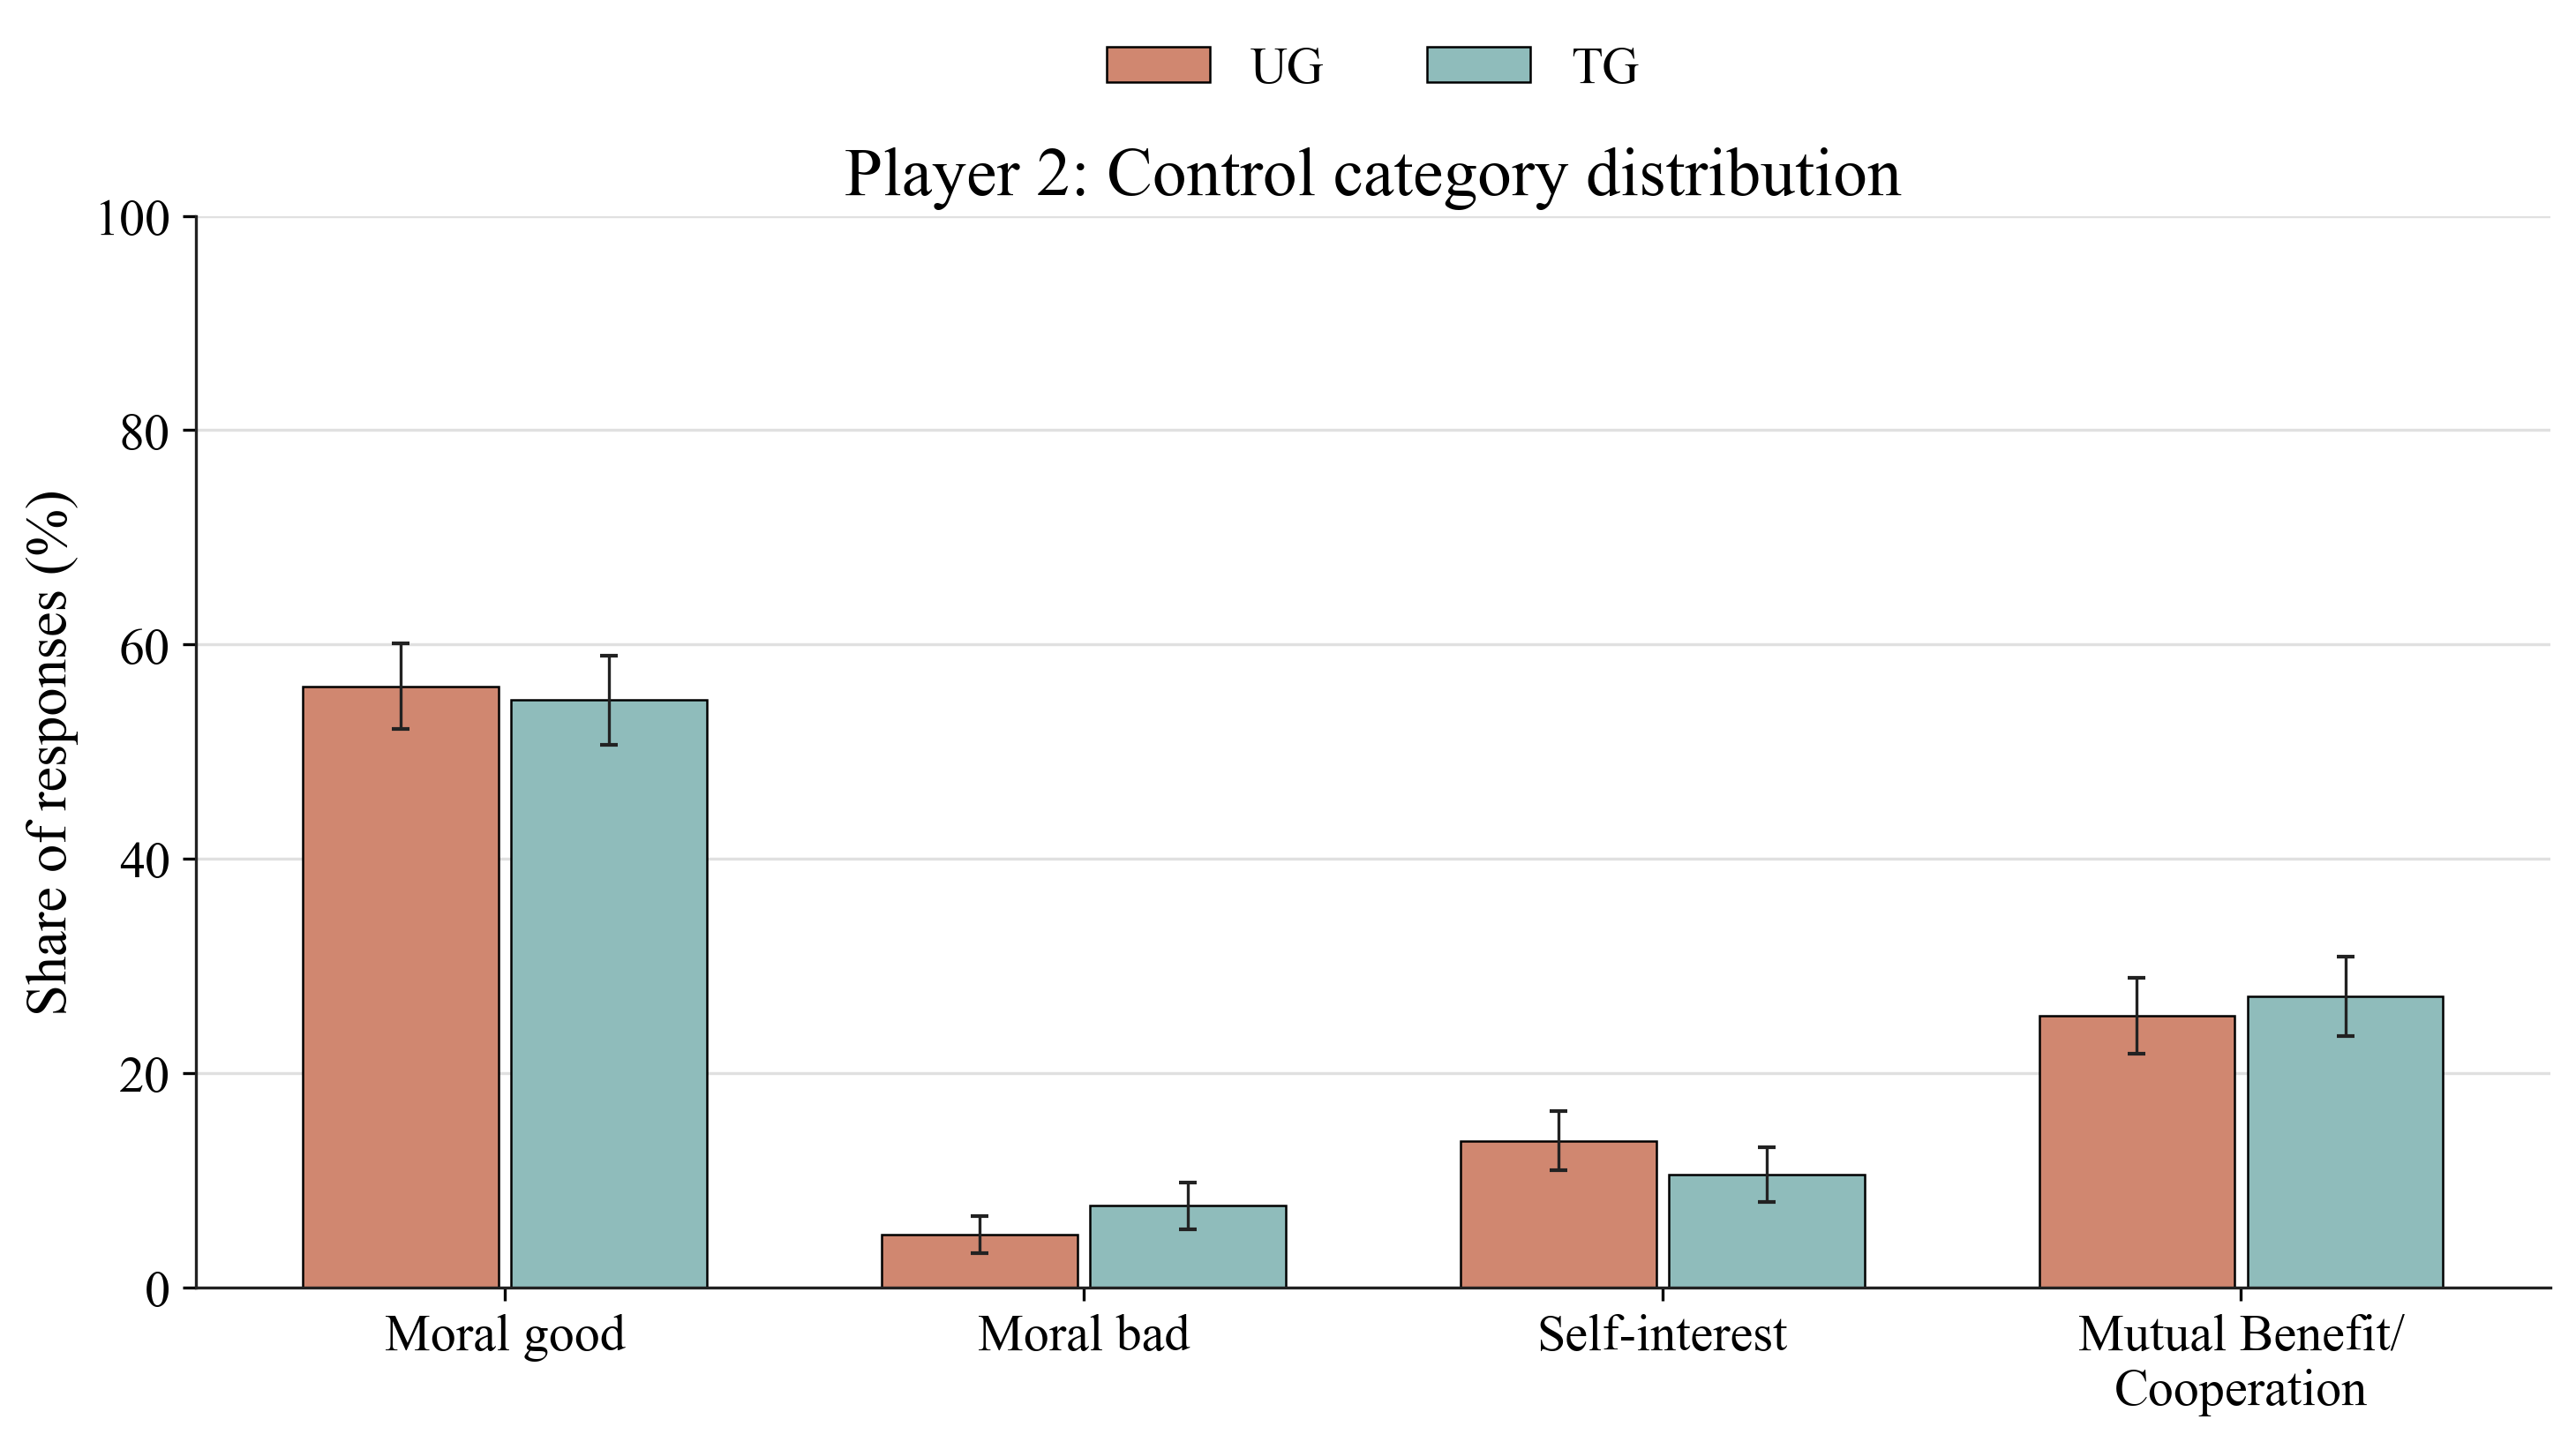
\includegraphics[width=0.82\textwidth]{player2_control_category_distribution_substantive_only.png}
\caption{Control-sample representation distributions for Player 2, excluding unclassified observations. Error bars show 95\% confidence intervals.}
\label{fig:appendix_player2_control_category}
\end{figure}

\begin{table}[!htbp]
\centering
\caption{\textbf{Player 2: Counterpart Proximity within Stated Reason Category}}
\label{tab:player2_sp_by_category}
\begin{tabular}{lcccc}
\toprule
Counterpart proximity & Moral good & Moral bad & Self-interest & Mutual Benefit/Cooperation \\
\midrule
Low social proximity & 48.6\% & 82.2\% & 91.0\% & 19.1\% \\
High social proximity & 51.4\% & 17.8\% & 9.0\% & 80.9\% \\
\bottomrule
\end{tabular}
\begin{flushleft}
\footnotesize Notes: Pooled across all games and treatments for Player 2. Columns report the distribution of counterpart proximity within each stated reason category and sum to 100\%.
\end{flushleft}
\end{table}


\begin{table}[!htbp]
\centering
\small
\renewcommand{\arraystretch}{1.2}
\caption{\textbf{Belief Sensitivity of Actions, by Representation Category}}
\label{tab:belief_sensitivity}
\begin{tabular}{ll rr rr}
\toprule
 & & \multicolumn{2}{c}{Control} & \multicolumn{2}{c}{All conditions (condition FE)} \\
\cmidrule(lr){3-4}\cmidrule(lr){5-6}
Game & Category & Slope & (SE) & Slope & (SE) \\
\midrule
UG & Moral & 0.010 & (0.020) & -0.003 & (0.016) \\
 & Self-interest & -0.108 & (0.096) & -0.093 & (0.048) \\
 & Mutual Benefit/Coop. & -0.083 & (0.319) & -0.128 & (0.089) \\
\midrule
TG & Moral & 0.306 & (0.095) & 0.319 & (0.045) \\
 & Self-interest & 0.451 & (0.144) & 0.465 & (0.086) \\
 & Mutual Benefit/Coop. & 0.264 & (0.098) & 0.128 & (0.045) \\
\bottomrule
\end{tabular}
\begin{flushleft}
\footnotesize Notes: OLS slopes of the Player 1 action (share) on the hypothetical belief at the one-third reference action, estimated separately by representation category; robust (HC1) standard errors. ``All conditions'' pools the four conditions with condition fixed effects. Slope-equality F-tests across categories: UG control $p=0.464$, UG pooled $p=0.002$, TG control $p=0.560$, TG pooled $p=0.000$. Model predictions: negative slopes in the UG, positive in the TG for every category (the equal-payoff norm anchor moves with the believed return); magnitude largest for Self-interest, whose material channel adds to the common anchor channel. The UG Mutual Benefit/Cooperation cell is very small and should be read accordingly.
\end{flushleft}
\end{table}


\begin{figure}[!htbp]
\centering
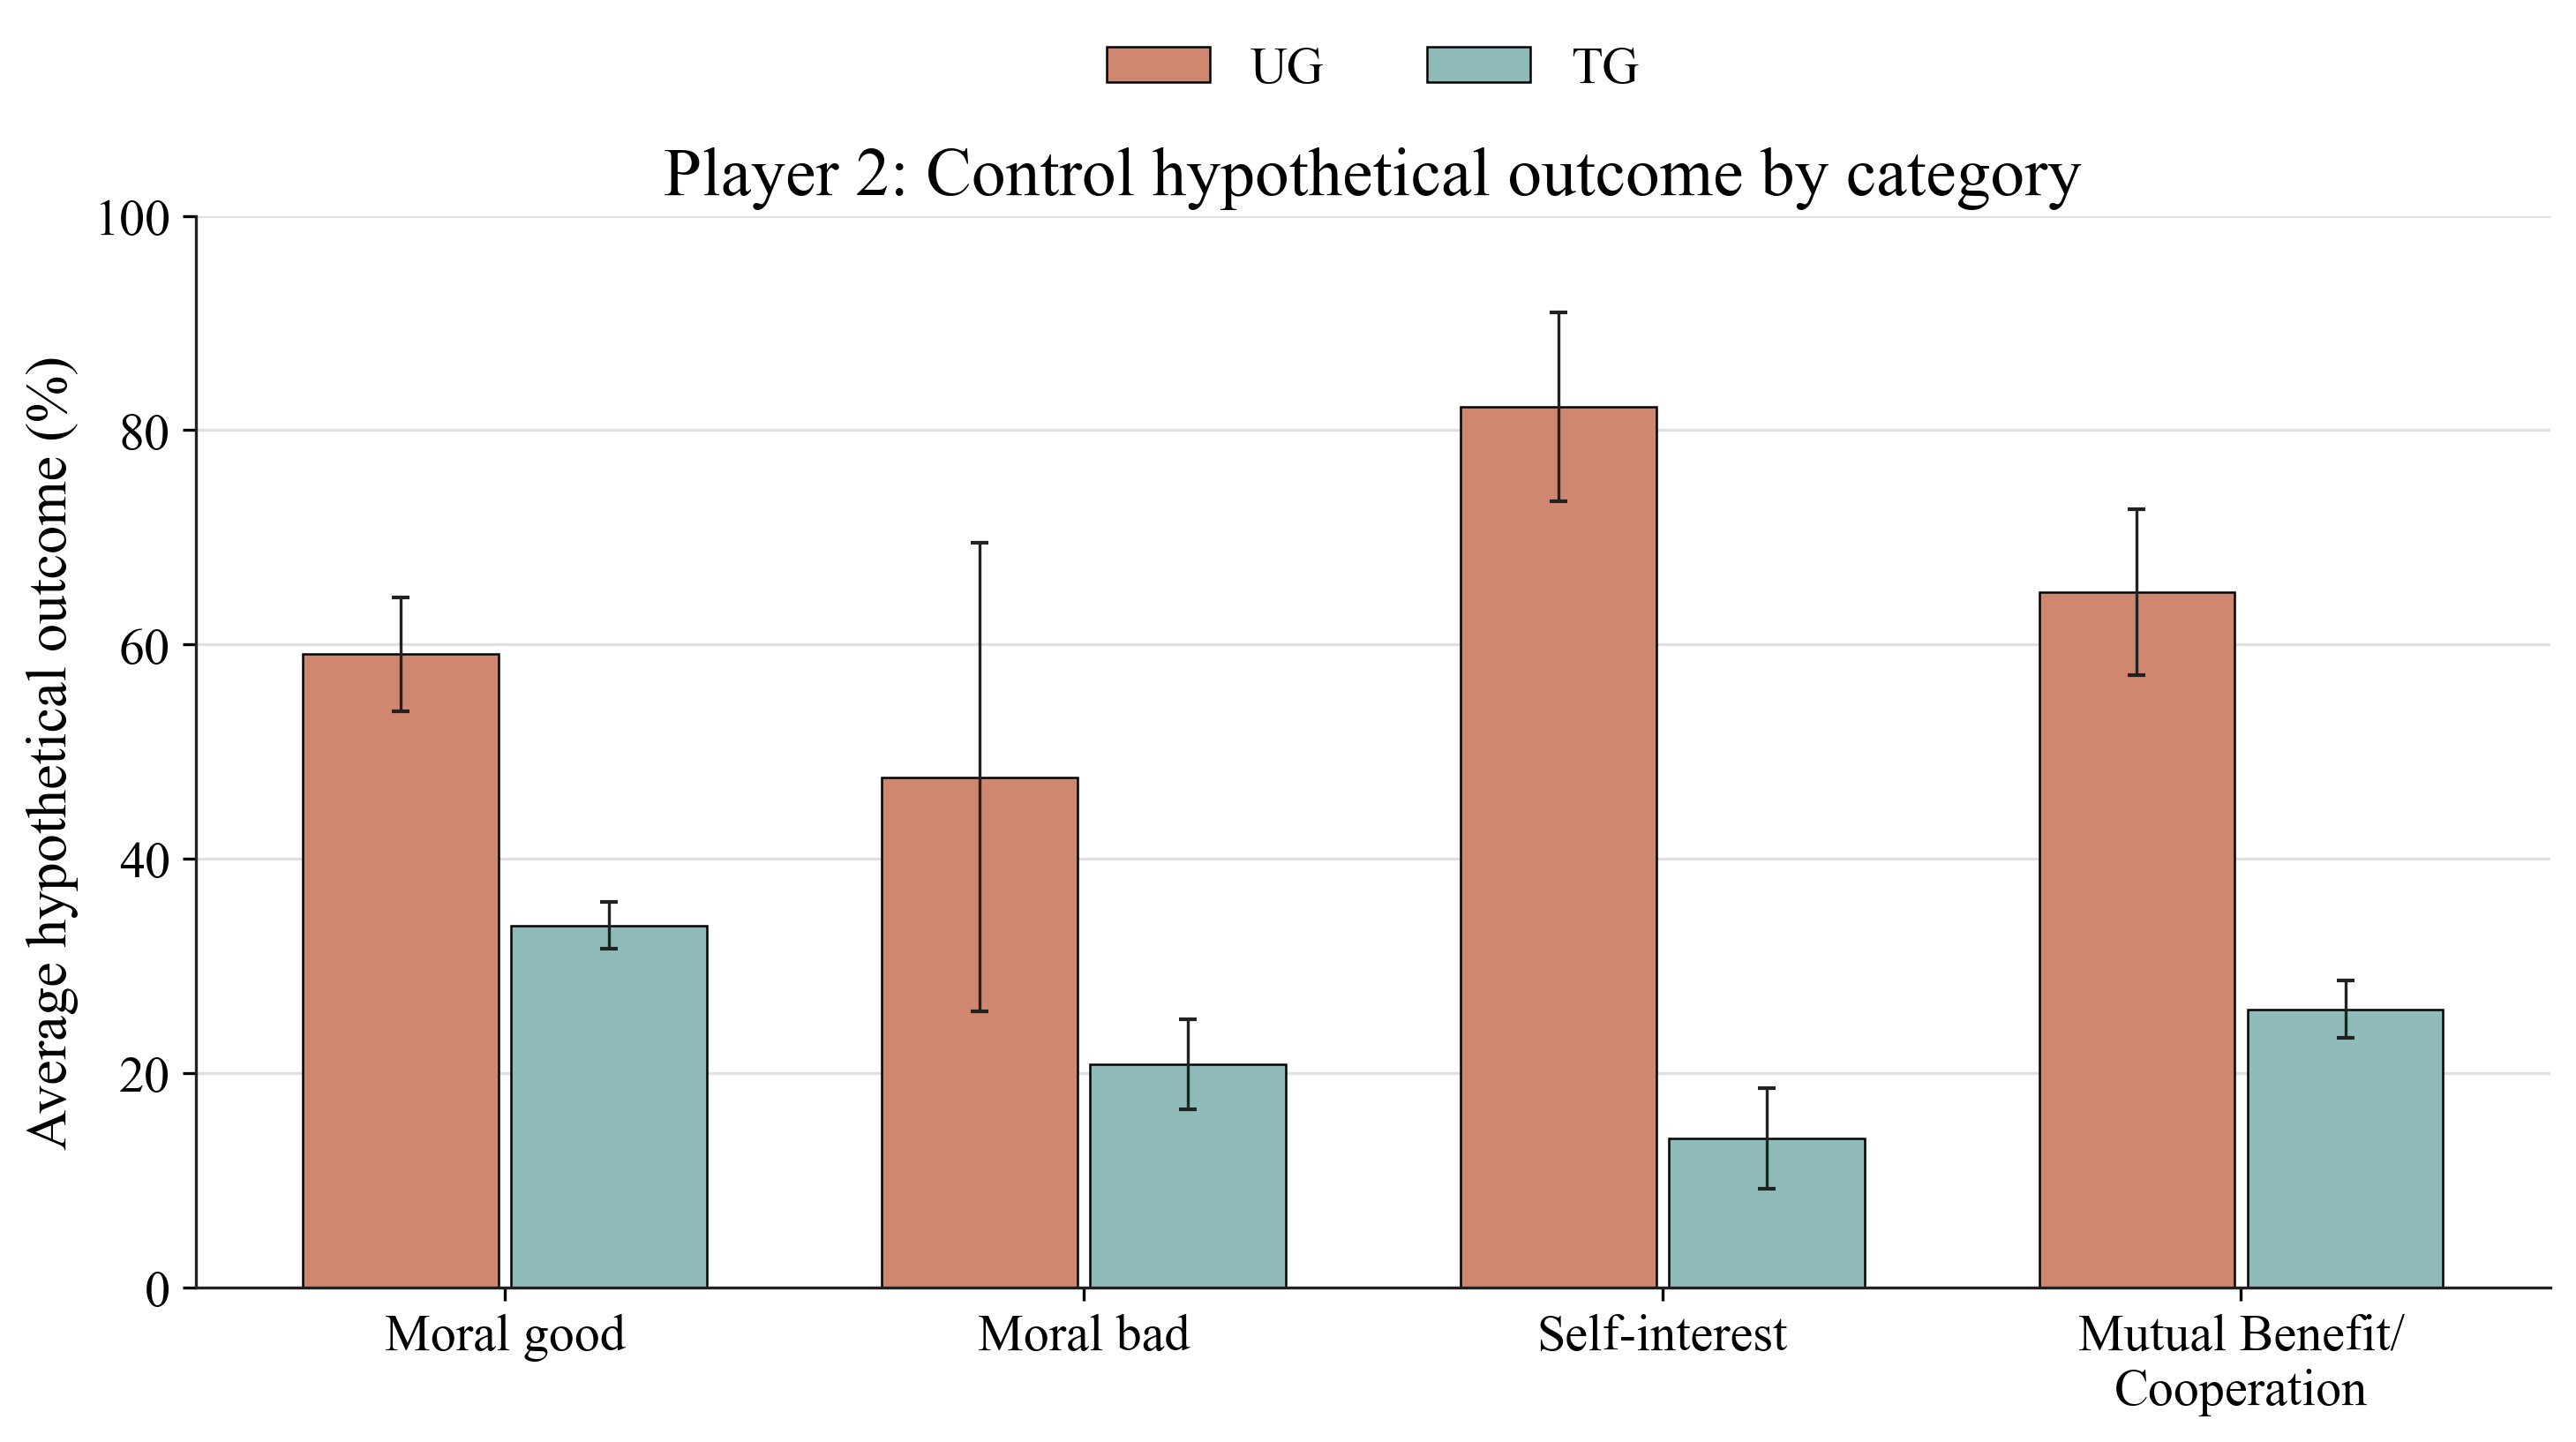
\includegraphics[width=0.82\textwidth]{player2_control_hp_outcome_by_category_substantive_only.png}
\caption{Control-sample hypothetical outcomes by category for Player 2. UG is measured using hypothetical acceptance and TG using hypothetical share sent. Error bars show 95\% confidence intervals.}
\label{fig:appendix_player2_control_outcome}
\end{figure}

\begin{figure}[!htbp]
\centering
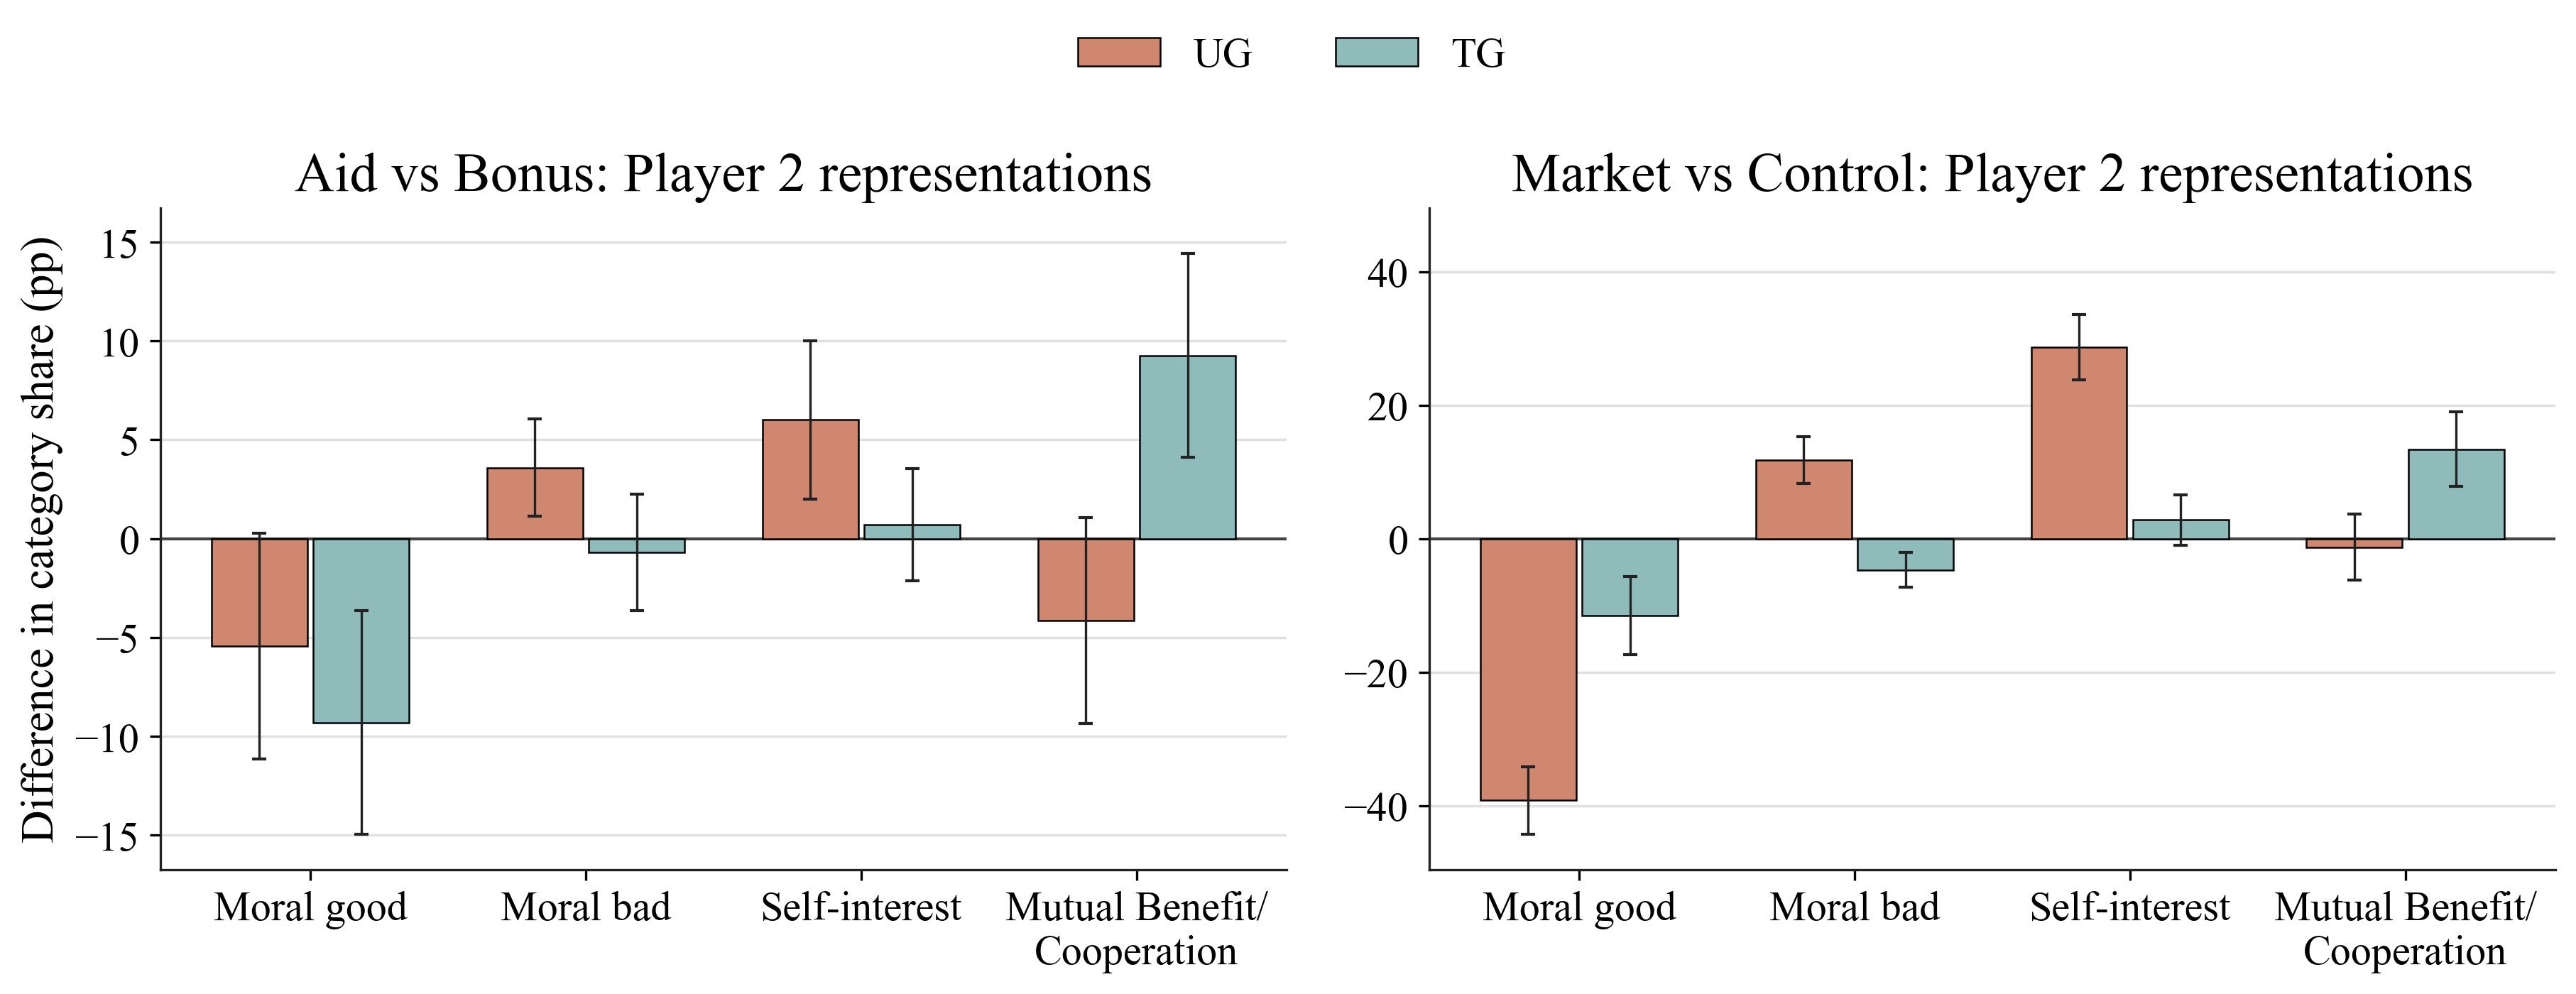
\includegraphics[width=0.96\textwidth]{appendix_player2_category_shifts.png}
\caption{Treatment-induced shifts in Player 2 category shares. Panels report Aid vs Bonus and Market vs Control. Error bars show 95\% confidence intervals.}
\label{fig:appendix_player2_category_shifts}
\end{figure}

\begin{table}[!htbp]
\centering
\caption{\textbf{Benchmark Regressions: Player 1, Forecast Error, Categories + Beliefs HP}}
\label{tab:cats_hp_cats_hp_fe_regs}
\begin{tabular}{lcc}
\toprule
 & (1) & (2) \\
 & UG & TG \\
\midrule
Self-interest & 0.129$^{***}$ & -0.017 \\
 & (0.019) & (0.016) \\
Mutual Benefit / Cooperation & 0.155$^{***}$ & 0.019$^{*}$ \\
 & (0.026) & (0.011) \\
No clear justification & 0.131$^{***}$ & 0.038 \\
 & (0.032) & (0.033) \\
Hypothetical beliefs & 0.469$^{***}$ & 0.517$^{***}$ \\
 & (0.032) & (0.026) \\
Constant & -0.400$^{***}$ & -0.189$^{***}$ \\
 & (0.018) & (0.012) \\
\midrule
Observations & 2279 & 1887 \\
$R^2$ & 0.139 & 0.183 \\
\bottomrule
\end{tabular}
\begin{flushleft}
\footnotesize Forecast Error is defined as Player 1 belief minus realized Player 2 behavior. Baseline category is Moral. Sample restricted to pooled Control, Market, Bonus, and Aid. Regressions include category dummies and hypothetical beliefs. $^{*}p<0.10$, $^{**}p<0.05$, $^{***}p<0.01$.
\end{flushleft}
\end{table}

\begin{table}[!htbp]
\centering
\caption{\textbf{Benchmark Regressions: Player 1, Hypothetical FE, Categories + Beliefs HP}}
\label{tab:cats_hp_cats_hp_hypfe_regs}
\begin{tabular}{lcc}
\toprule
 & (1) & (2) \\
 & UG & TG \\
\midrule
Self-interest & -0.061$^{**}$ & -0.037$^{***}$ \\
 & (0.025) & (0.013) \\
Mutual Benefit / Cooperation & -0.017 & -0.030$^{***}$ \\
 & (0.035) & (0.010) \\
No clear justification & -0.066 & -0.015 \\
 & (0.043) & (0.028) \\
Hypothetical beliefs & 0.933$^{***}$ & 0.996$^{***}$ \\
 & (0.043) & (0.023) \\
Constant & -0.627$^{***}$ & -0.317$^{***}$ \\
 & (0.024) & (0.010) \\
\midrule
Observations & 2279 & 1887 \\
$R^2$ & 0.176 & 0.513 \\
\bottomrule
\end{tabular}
\begin{flushleft}
\footnotesize Hypothetical FE is defined as Player 1 hypothetical belief minus the corresponding hypothetical Player 2 response. Baseline category is Moral. Sample restricted to pooled Control, Market, Bonus, and Aid. Regressions include category dummies and hypothetical beliefs. $^{*}p<0.10$, $^{**}p<0.05$, $^{***}p<0.01$.
\end{flushleft}
\end{table}


\begin{table}[!htbp]
\centering
\caption{\textbf{Instability calibration regressions, Categories Only}}
\label{tab:cats_only_instability_regs}
\begin{tabular}{lccc}
\toprule
& All & Player 1 & Player 2 \\
\midrule
Intercept & 0.007 & 0.021** & 0.015 \\
& (0.013) & (0.009) & (0.019) \\
Predicted & 1.413*** & 2.772*** & 1.218*** \\
& (0.177) & (0.223) & (0.179) \\
Observations & 18 & 10 & 8 \\
$R^2$ & 0.799 & 0.951 & 0.886 \\
\bottomrule
\end{tabular}

\vspace{0.2cm}
\begin{minipage}{0.9\textwidth}
\footnotesize Notes: Unit of observation is an outcome-by-comparison cell from the fitted-values exercise. Each column reports the regression of the actual treatment effect on the predicted treatment effect. Standard errors in parentheses. $^*$ $p<0.1$, $^{**}$ $p<0.05$, $^{***}$ $p<0.01$.
\end{minipage}
\end{table}


\clearpage

\section{Within-Subject Evidence from the Dictator Game}
\label{app:within}

The dictator-game pre-registration (AsPredicted \#261370) included three within-subject arms of 600 participants each (599 complete pairs in the DG-KW market arm), all without stories: (i) game fixed at DG-KW, frame varying between abstract and market; (ii) game fixed at DG-LT, frame varying between abstract and market; (iii) frame fixed at abstract, game varying between DG-KW and DG-LT\@. Order was randomized; order effects are small---within condition, mean shares sent differ by at most 2.5 percentage points between first and second decisions---and order enters all specifications below.
% NOTE 2026-07-10: previous claim ``order effects are sizable (participants give more in their second decision when DG-LT comes first)'' was contradicted by the microdata (cell means in paper_tables/validation_within_stats.txt; LT-first second decisions are 4.3pp LOWER than KW-first second decisions) and rested on the unidentified LTFirst row of the within tables, since dropped. AA confirmed (2026-07-10) that no observations were excluded: 599 is the total number of complete pairs in the DG-KW market arm. These arms establish at the individual level the connection between representation switching and behavioral switching that the between-subject design establishes at the treatment level.
% NOTE 2026-07-12 (NG: "sarebbe ottimo vedere cosa otteniamo se guardiamo ad instability in beliefs and representations"): NOT measurable in these data --- the within arms are DG-only and dictator arms have no belief elicitation (AA's inventory, reproduced from his microdata 07-10). What exists within is behavior + representations, i.e., exactly this appendix. Model prediction for a FUTURE within-subject UG/TG arm: beliefs are prototype content, so belief switching should concentrate among category switchers --- flagged to NG as a follow-up design, not current-data work. Do NOT restructure this appendix before AA confirms the three-arm inventory (his "due esperimenti" vs the 3x600 in validation_within_stats.txt).

Table~\ref{tab:within_switching_summary} summarizes switching behavior. When the same participant plays DG-KW and DG-LT under the abstract frame, 46.2\% change their choice (share sent) and 22.7\% change their representation category; when the frame switches between abstract and market with the game fixed, 73.1\% (DG-KW) and 82.3\% (DG-LT) change their choice and over half change their category. In all three arms, choice switching is strongly predicted by category switching: participants whose representation category changes are 14--44 percentage points more likely to change their choice than participants whose category is stable (linear-probability estimates: 0.44, robust SE 0.04, in the DG-KW/DG-LT arm; 0.19, SE 0.04, and 0.14, SE 0.03, in the two market arms; all $p<0.001$). Choice switching counts any change in the share sent, so it includes small adjustments; the conditional contrast between category switchers and stayers is the informative statistic.

\begin{table}[!htbp]
\centering
\caption{\textbf{Within-Subject Switching in the Dictator Game}}
\label{tab:within_switching_summary}
\resizebox{0.98\textwidth}{!}{%
\begin{tabular}{lcccccc}
\toprule
 & & \multicolumn{3}{c}{Share switching} & \multicolumn{2}{c}{P(choice switch $\mid$ category)} \\
\cmidrule(lr){3-5} \cmidrule(lr){6-7}
Comparison & $N$ pairs & Choice & Category & Social proximity & Switched & Stayed \\
\midrule
DG-KW vs DG-LT (abstract frame) & 600 & 46.2\% & 22.7\% & 40.5\% & 80.1\% & 36.2\% \\
Market vs Control (DG-KW) & 599 & 73.1\% & 51.6\% & 66.4\% & 82.2\% & 63.4\% \\
Market vs Control (DG-LT) & 600 & 82.3\% & 55.0\% & 62.0\% & 88.5\% & 74.8\% \\
\bottomrule
\end{tabular}
}
\begin{flushleft}
\footnotesize Notes: Each participant makes two dictator-game decisions. In the first row, both decisions use the abstract (control) frame and the game varies (KW vs LT); in the second and third rows, the game is fixed and the frame varies (abstract vs market). ``Choice'' switching is any change in the share sent; ``Category'' switching is a change in the reason-based representation category (Moral, Self-interest, Mutual Benefit/Cooperation, No clear justification); ``Social proximity'' switching is a change in the social-proximity class of the representation. The last two columns report the probability of a choice switch conditional on the representation category switching or staying fixed.
\end{flushleft}
\end{table}


\begin{figure}[!htbp]
\centering
% Regenerated by 04 (2026-07-15) from within/within_switching_results.xlsx; reproduces
% every percentage printed on the original within/choice_switch_control_kw_first.png,
% which had no generator in the repo and is kept there untouched.
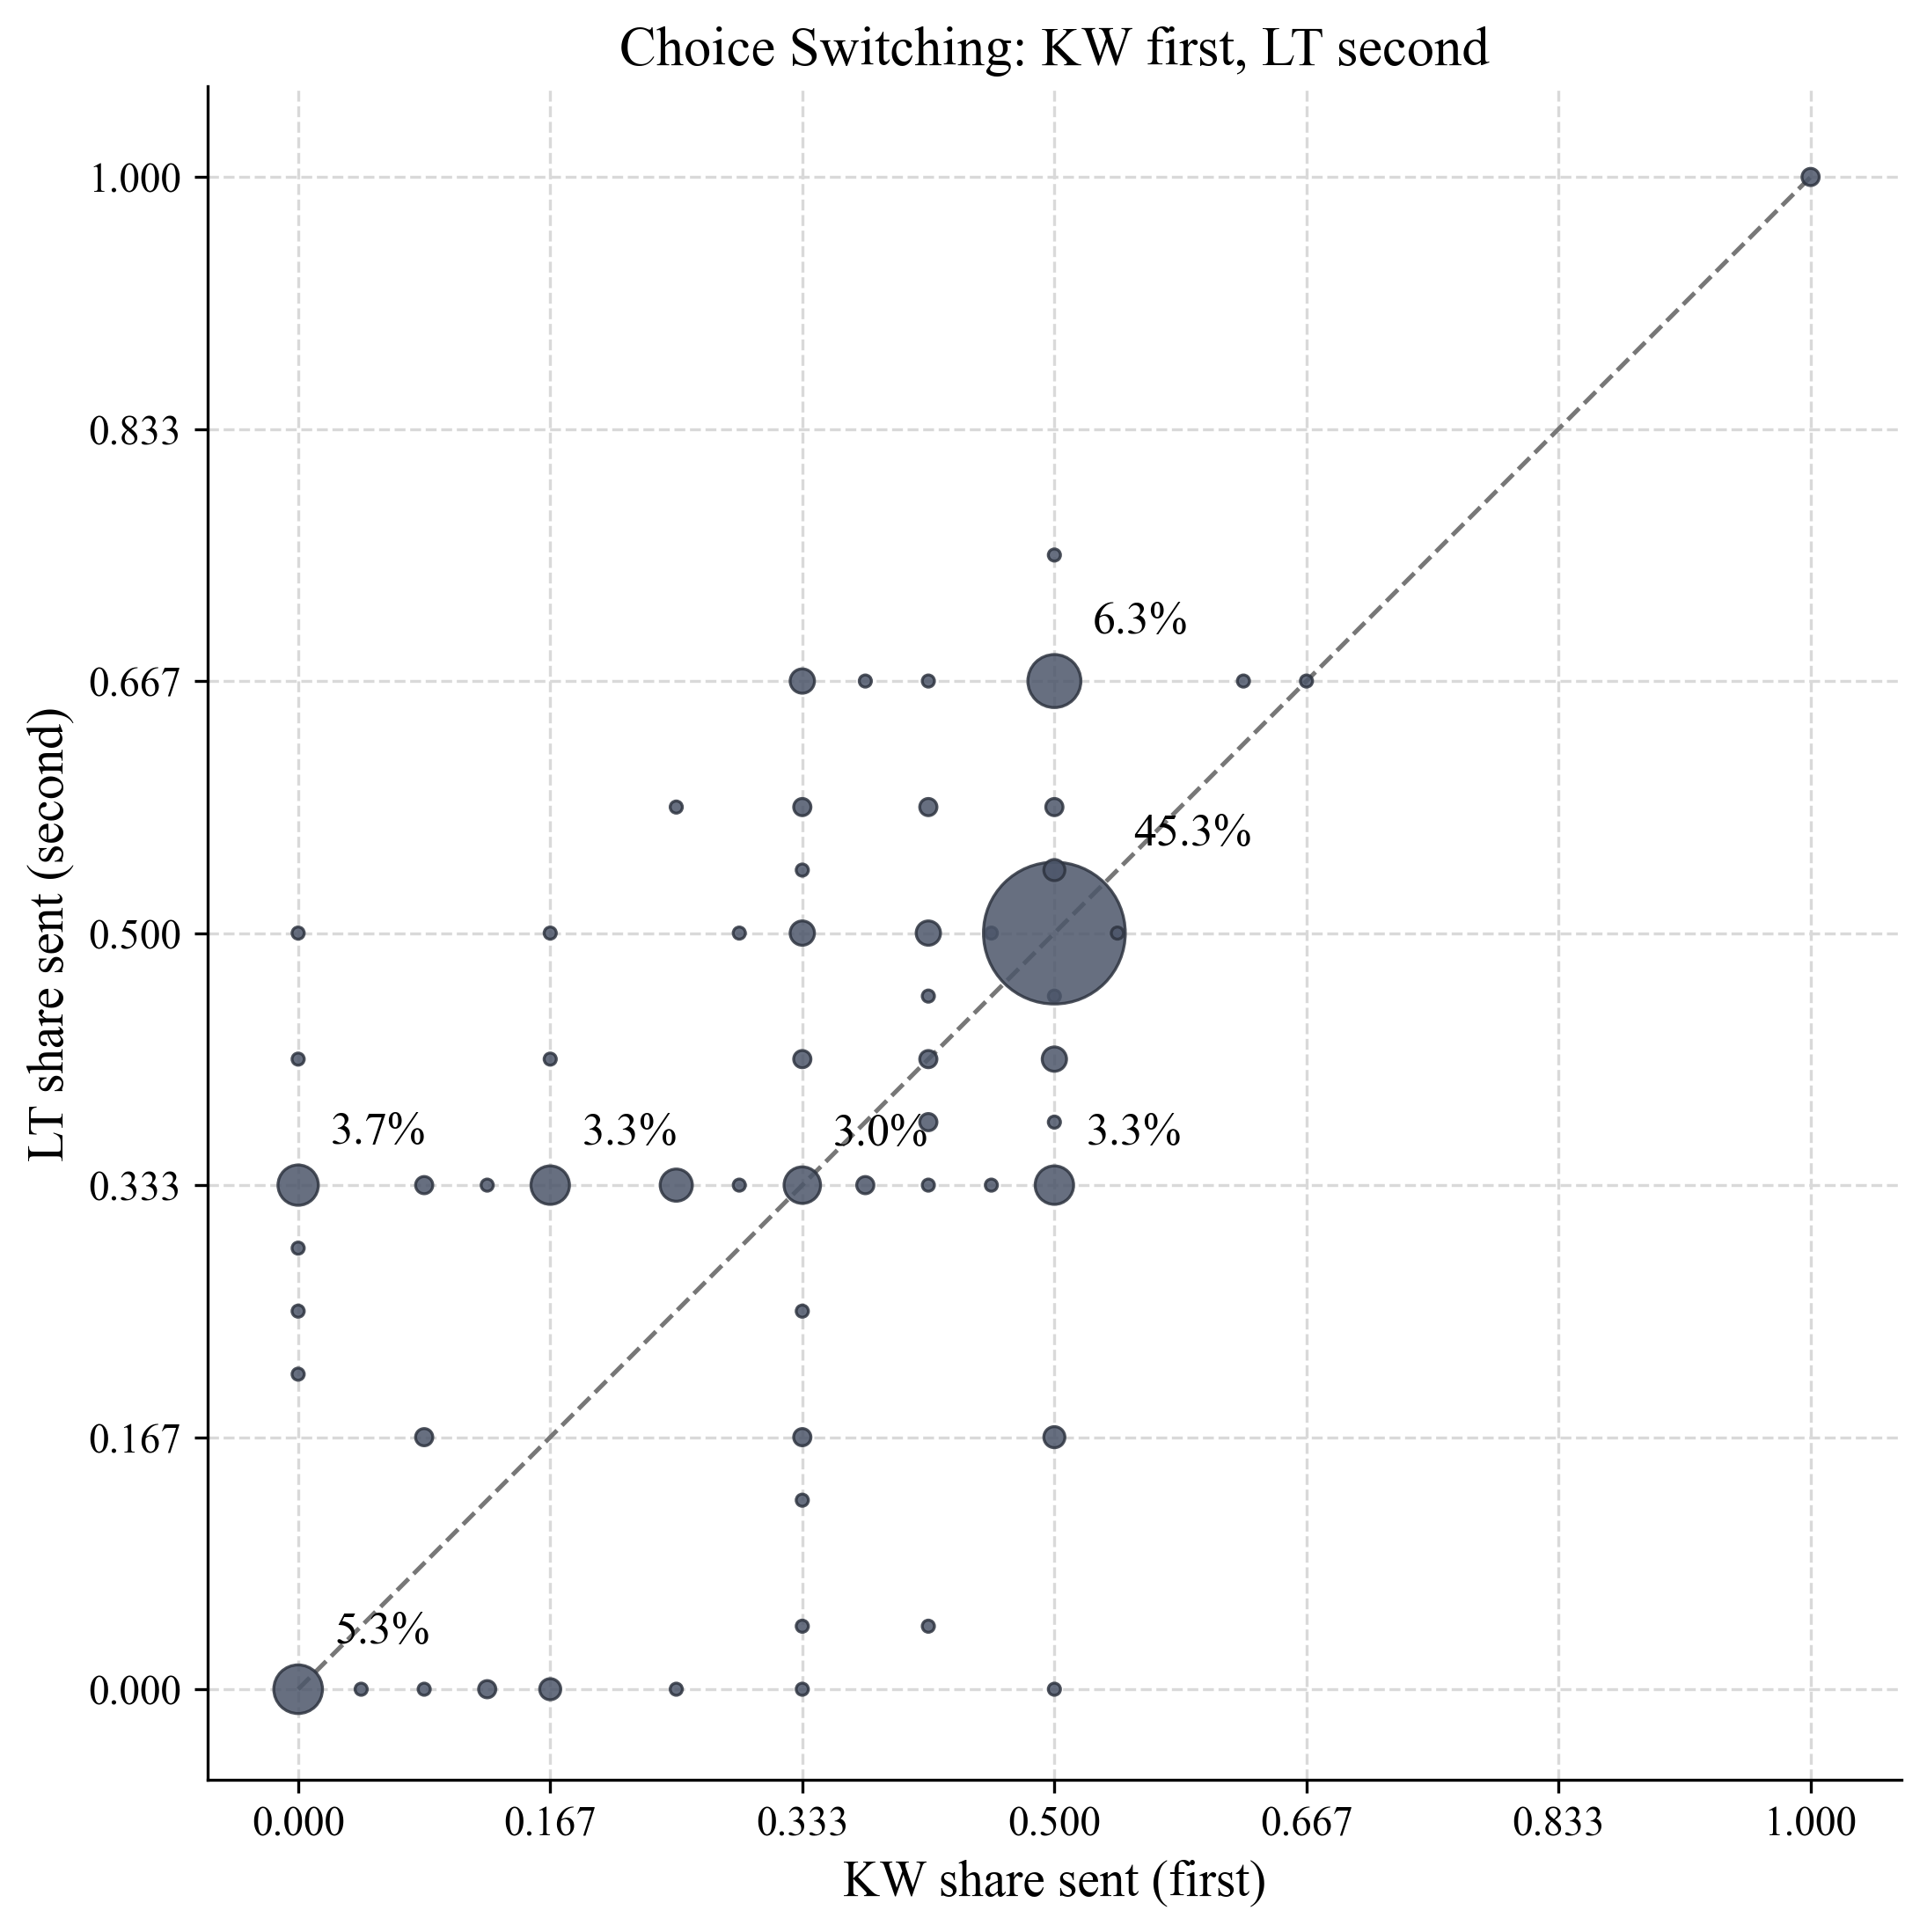
\includegraphics[width=0.80\textwidth]{within_choice_switch_kw_first.png}
\caption{Within-subject choice switching between DG-KW (first decision) and DG-LT (second decision), control frame. Point size is proportional to the share of participants at each pair of choices; the dashed line marks unchanged choices. The mass below the diagonal at high KW shares and above it at low KW shares shows regression toward the LT default.}
\label{fig:within_choice_switch}
\end{figure}

Tables~\ref{tab:within_control_regressions}--\ref{tab:within_market_category_regressions} report within-subject regressions with participant fixed effects. Holding the participant fixed, moving from DG-LT to DG-KW lowers the share sent by 3.3--3.6 percentage points, and moving from the abstract to the market frame lowers it substantially; representation categories predict behavior within participant, with self-interested representations associated with significantly lower transfers. % DONE 2026-07-10 via 06_validation_and_within_checks.py: every FE-identified coefficient in all four columns of both tables (KW/Market, order interactions, HighSP, category dummies, R2, N) reproduces to the third decimal from missingdata/within_all_long_categorized.xlsx under strict FE (LSDV) with participant-clustered SEs --- the tables ARE participant fixed effects.
% DONE 2026-07-10 (AA reply, round 3): AA confirmed the LTFirst=0.104 (0.008) and ControlFirst=0.184 (0.013) rows came from statsmodels' generalized (pseudo-inverse) solution to the rank-deficient FE design --- not identified, not to be interpreted; order effects require a no-FE spec with participant-clustered SEs. Rows dropped from both tables; the no-FE clustered estimates (+0.019 (0.015) / +0.009 (0.013), from 06_validation_and_within_checks.py) now appear in the table notes.

\begin{table}[!htbp]
\centering
\caption{\textbf{Within-Subject Regressions}: Control sample, LT vs.\ KW}
\label{tab:within_control_regressions}
\begin{tabular}{lcccc}
\toprule
 & (1) & (2) & (3) & (4) \\
 & \multicolumn{4}{c}{Share Sent P1} \\
\cmidrule(lr){2-5}
\midrule
KW & -0.036$^{***}$ & -0.035$^{***}$ & -0.033$^{***}$ & -0.033$^{***}$ \\
 & (0.011) & (0.011) & (0.010) & (0.010) \\
KW x LTFirst & -0.026 & -0.026 & -0.033$^{**}$ & -0.033$^{**}$ \\
 & (0.016) & (0.016) & (0.015) & (0.015) \\
HighSP &  & 0.011 &  & -0.004 \\
 &  & (0.015) &  & (0.015) \\
Mutual Benefit / Cooperation &  &  & -0.070 & -0.070 \\
 &  &  & (0.072) & (0.072) \\
Self-interest &  &  & -0.091$^{***}$ & -0.093$^{***}$ \\
 &  &  & (0.026) & (0.026) \\
No clear justification &  &  & -0.053 & -0.054 \\
 &  &  & (0.039) & (0.040) \\
Participant fixed effects & Yes & Yes & Yes & Yes \\
Observations & 1200 & 1200 & 1200 & 1200 \\
Participants & 600 & 600 & 600 & 600 \\
$R^2$ & 0.867 & 0.868 & 0.877 & 0.877 \\
\bottomrule
\end{tabular}
\begin{flushleft}
\footnotesize Outcome is DG share sent by Player 1, defined as $1-\texttt{allocation}/12$. Models use the within-control LT/KW sample only. All specifications include participant fixed effects and cluster standard errors by participant. Baseline text category is Moral. HighSP equals 1 if \texttt{sp\_num}>1. LTFirst equals 1 when LT was shown before KW\@; its main effect is collinear with the participant fixed effects and therefore not identified. Estimated without fixed effects (standard errors clustered by participant), the LTFirst level effect is $+0.019$ (SE $0.015$). $^{*}p<0.10$, $^{**}p<0.05$, $^{***}p<0.01$.
\end{flushleft}
\end{table}

\begin{table}[!htbp]
\centering
\caption{\textbf{Within-Subject Regressions}: Market vs.\ Control within subject}
\label{tab:within_market_regressions}
\begin{tabular}{lcccc}
\toprule
 & (1) & (2) & (3) & (4) \\
 & \multicolumn{4}{c}{Share Sent P1} \\
\cmidrule(lr){2-5}
\midrule
Market & -0.160$^{***}$ & -0.139$^{***}$ & -0.135$^{***}$ & -0.126$^{***}$ \\
 & (0.017) & (0.018) & (0.018) & (0.019) \\
Market x ControlFirst & 0.016 & 0.017 & 0.017 & 0.017 \\
 & (0.025) & (0.025) & (0.024) & (0.024) \\
HighSP &  & 0.113$^{***}$ &  & 0.062$^{***}$ \\
 &  & (0.021) &  & (0.021) \\
Mutual Benefit / Cooperation &  &  & -0.076$^{**}$ & -0.073$^{**}$ \\
 &  &  & (0.033) & (0.033) \\
Self-interest &  &  & -0.197$^{***}$ & -0.177$^{***}$ \\
 &  &  & (0.022) & (0.023) \\
No clear justification &  &  & -0.084$^{**}$ & -0.068$^{**}$ \\
 &  &  & (0.034) & (0.034) \\
Participant fixed effects & Yes & Yes & Yes & Yes \\
Observations & 2398 & 2398 & 2398 & 2398 \\
Participants & 1199 & 1199 & 1199 & 1199 \\
$R^2$ & 0.597 & 0.614 & 0.642 & 0.647 \\
\bottomrule
\end{tabular}
\begin{flushleft}
\footnotesize Outcome is DG share sent by Player 1, defined as $1-\texttt{allocation}/12$. Models use the within-subject Market vs.\ Control sample pooled across the fixed-game designs. All specifications include participant fixed effects and cluster standard errors by participant. Baseline text category is Moral. HighSP equals 1 if \texttt{sp\_num}>1. ControlFirst equals 1 when Control was shown before Market; its main effect is collinear with the participant fixed effects and therefore not identified. Estimated without fixed effects (standard errors clustered by participant), the ControlFirst level effect is $+0.009$ (SE $0.013$). $^{*}p<0.10$, $^{**}p<0.05$, $^{***}p<0.01$.
\end{flushleft}
\end{table}

\begin{table}[!htbp]
\centering
\caption{\textbf{Within-Subject Category Regressions}: Control sample, LT vs.\ KW}
\label{tab:within_control_category_regressions}
\begin{tabular}{lccc}
\toprule
 & \shortstack{Mutual Benefit /\\ Cooperation} & Self-interest & \shortstack{No clear\\ justification} \\
 & \multicolumn{3}{c}{Outcome category relative to Moral} \\
\cmidrule(lr){2-4}
\midrule
KW & 1.633 & 0.250$^{*}$ & -0.711$^{**}$ \\
 & (1.105) & (0.142) & (0.329) \\
LTFirst & 1.391 & 0.217 & -0.912$^{**}$ \\
 & (1.128) & (0.206) & (0.388) \\
KW x LTFirst & -2.379$^{*}$ & -0.480$^{**}$ & 0.753 \\
 & (1.410) & (0.202) & (0.489) \\
Observations & 1200 & 1200 & 1200 \\
Participants & 600 & 600 & 600 \\
Pseudo $R^2$ & 0.009 & 0.009 & 0.009 \\
\bottomrule
\end{tabular}
\begin{flushleft}
\footnotesize Outcome is the main reason category. Entries are multinomial-logit coefficients relative to the omitted category Moral. The sample is the within-control LT/KW design only. Regressors are KW, LTFirst, and their interaction. Standard errors are clustered by participant. LTFirst equals 1 when LT was shown before KW\@. $^{*}p<0.10$, $^{**}p<0.05$, $^{***}p<0.01$.
\end{flushleft}
\end{table}

\begin{table}[!htbp]
\centering
\caption{\textbf{Within-Subject Category Regressions}: Market vs.\ Control within subject}
\label{tab:within_market_category_regressions}
\begin{tabular}{lccc}
\toprule
 & \shortstack{Mutual Benefit /\\ Cooperation} & Self-interest & \shortstack{No clear\\ justification} \\
 & \multicolumn{3}{c}{Outcome category relative to Moral} \\
\cmidrule(lr){2-4}
\midrule
Market & 3.150$^{***}$ & 0.720$^{***}$ & 1.553$^{***}$ \\
 & (0.333) & (0.123) & (0.184) \\
ControlFirst & -1.322$^{**}$ & -0.237$^{*}$ & -0.661$^{**}$ \\
 & (0.664) & (0.131) & (0.262) \\
Market x ControlFirst & 0.258 & -0.094 & 0.351 \\
 & (0.679) & (0.167) & (0.279) \\
KW design & -0.278 & -0.106 & -0.072 \\
 & (0.172) & (0.108) & (0.152) \\
Observations & 2398 & 2398 & 2398 \\
Participants & 1199 & 1199 & 1199 \\
Pseudo $R^2$ & 0.070 & 0.070 & 0.070 \\
\bottomrule
\end{tabular}
\begin{flushleft}
\footnotesize Outcome is the main reason category. Entries are multinomial-logit coefficients relative to the omitted category Moral. The sample is the within-subject Market vs.\ Control design pooled across the fixed-game designs. Regressors are Market, ControlFirst, their interaction, and a KW-design indicator. Standard errors are clustered by participant. ControlFirst equals 1 when Control was shown before Market. $^{*}p<0.10$, $^{**}p<0.05$, $^{***}p<0.01$.
\end{flushleft}
\end{table}

\clearpage

\section{Representations from Hypothetical Allocations}
\label{app:hp}
% NOTE 2026-07-10 (AA email): the hypothetical-allocation answers were never classified with the NEW category scheme (OpenAI credit issues), so no reclassified microdata exists; this appendix rests on the v1 fine-grained classification. Independent reproduction deferred as a robustness item, per AA --- revisit in a second round.

The dictator-game pre-registration specified a second measure of representations, elicited before the transfer decision: participants were shown hypothetical final allocations and asked to describe a real-world situation they find similar to each. The answers were classified with the same LLM-plus-validation procedure into social-proximity categories and into fine-grained moral categories (Need, Egalitarian, Generous, Neutral, Entitlement, Greedy, Theft). Because this measure is anchored to \emph{allocations} rather than to the participant's chosen action, it is less susceptible to ex-post rationalization of the choice. This appendix shows that it delivers the same conclusions as the reasons-based measure, both for the KW--LT comparison of the Introduction and Section~\ref{sec:kwlt} and for the market treatment.

\subsection{DG-KW versus DG-LT}

\begin{table}[!htbp]
\centering
\caption{Distribution of social-proximity categories (hypothetical-allocation measure) and mean allocation kept by the dictator, by game. Control condition.}
\label{tab:social_proximity_hpmin_kw_lt}
\renewcommand{\arraystretch}{1.1}
\footnotesize
\setlength{\tabcolsep}{6pt}
\begin{tabular}{l r r r r}
\toprule
 & \multicolumn{2}{c}{\textbf{Share of responses}}
 & \multicolumn{2}{c}{\textbf{Mean Allocation}} \\
\cmidrule(lr){2-3} \cmidrule(lr){4-5}
\textbf{Social proximity} & KW & LT & KW & LT \\
\midrule
No mention of recipient & 26.50\% & 31.00\% & 8.74 & 7.39 \\
Abstract stranger        & 28.00\% & 28.50\% & 9.31 & 7.10 \\
Anonymous peer           & 17.50\% & 19.00\% & 6.00 & 6.24 \\
Teammate / coworker      & 7.50\%  & 5.50\%  & 6.60 & 7.09 \\
Friend                   & 20.50\% & 16.00\% & 6.83 & 6.14 \\
\bottomrule
\end{tabular}
\end{table}

\begin{table}[!htbp]
\centering
\caption{Allocation kept by the dictator and allocation-specific outcomes, by social proximity (hypothetical-allocation measure): OLS estimates, control condition. High SP indicates a socially close counterpart. Standard errors in parentheses. ${}^{***}p<0.01$, ${}^{**}p<0.05$.}
\label{tab:highsp_regressions_hpmin}
\renewcommand{\arraystretch}{1.1}
\footnotesize
\setlength{\tabcolsep}{6pt}
\begin{tabular}{lcccccc}
\toprule
 & Mean Allocation & =12 & $>$8 & =8 & =6 & =4 \\
\midrule
High SP &
$-1.703^{***}$ &
$-0.228^{***}$ &
$-0.299^{***}$ &
$-0.028$ &
$0.357^{***}$ &
$0.006$ \\
 & (0.220) & (0.034) & (0.039) & (0.034) & (0.047) & (0.019) \\
Constant &
$8.101^{***}$ &
$0.246^{***}$ &
$0.351^{***}$ &
$0.145^{***}$ &
$0.364^{***}$ &
$0.035^{***}$ \\
 & (0.144) & (0.022) & (0.026) & (0.022) & (0.031) & (0.013) \\
\midrule
Observations & 400 & 400 & 400 & 400 & 400 & 400 \\
$R^{2}$       & 0.131 & 0.102 & 0.126 & 0.002 & 0.125 & 0.000 \\
\bottomrule
\end{tabular}
\end{table}

\begin{table}[!htbp]
\centering
\caption{Symmetrized decomposition of mean differences between DG-KW and DG-LT into a representation component (differences in the distribution of social proximity) and a behavior component (differences in allocations conditional on social proximity). The decomposition is a descriptive accounting; no sampling uncertainty is attached.}
\label{tab:decomposition_sym_kw_lt}
\begin{tabular}{lccc}
\toprule
\textbf{Variable} & \textbf{Observed Diff} & \textbf{Representation Component} & \textbf{Behavior Component} \\
\midrule
\multicolumn{4}{l}{\textbf{KW $-$ LT}} \\
Mean Allocation   & 0.998   & 0.491   & 0.506 \\
Allocation = 4    & $-$0.065 & $-$0.032 & $-$0.033 \\
Allocation = 6    & $-$0.035 & $-$0.019 & $-$0.016 \\
Allocation = 8    & $-$0.075 & $-$0.036 & $-$0.039 \\
Allocation $>8$   & 0.205   & 0.102   & 0.103 \\
Allocation $=12$   & 0.105   & 0.051   & 0.054 \\
\bottomrule
\end{tabular}
\end{table}

\begin{table}[!htbp]
\centering
\caption{Distribution of moral categories (hypothetical-allocation measure) and mean allocation kept by the dictator, by game. Control condition.}
\label{tab:moral_kw_lt}
\renewcommand{\arraystretch}{1.1}
\footnotesize
\setlength{\tabcolsep}{6pt}
\begin{tabular}{l r r r r}
\toprule
 & \multicolumn{2}{c}{\textbf{Share of responses}}
 & \multicolumn{2}{c}{\textbf{Mean Allocation}} \\
\cmidrule(lr){2-3} \cmidrule(lr){4-5}
\textbf{Moral category} & KW & LT & KW & LT \\
\midrule
Need        & 2.50\%  & 1.00\%  & 11.40 & 6.00 \\
Egalitarian & 32.00\% & 27.50\% & 6.02  & 5.91 \\
Generous    & 33.00\% & 37.50\% & 7.43  & 6.03 \\
Neutral     & 8.50\%  & 11.00\% & 8.00  & 7.48 \\
Entitlement & 10.50\% & 11.00\% & 9.90  & 8.48 \\
Greedy      & 13.00\% & 8.00\%  & 10.96 & 8.75 \\
Theft       & 0.50\%  & 4.00\%  & 12.00 & 11.75 \\
\bottomrule
\end{tabular}
\end{table}

\begin{table}[!htbp]
\centering
\caption{Allocation kept by the dictator and allocation-specific outcomes, by moral category (hypothetical-allocation measure): OLS estimates, control condition. Baseline category is Neutral. Standard errors in parentheses. ${}^{***}p<0.01$, ${}^{**}p<0.05$, ${}^{*}p<0.10$.}
\label{tab:moral_regressions}
\renewcommand{\arraystretch}{1.1}
\footnotesize
\setlength{\tabcolsep}{6pt}
\begin{tabular}{lcccccc}
\toprule
 & Mean Allocation & =12 & $>$8 & =8 & =6 & =4 \\
\midrule
Generous &
$-1.021^{***}$ &
$-0.144^{***}$ &
$-0.103^{*}$ &
$-0.169^{***}$ &
$0.278^{***}$ &
$-0.009$ \\
 & (0.315) & (0.053) & (0.060) & (0.058) & (0.073) & (0.034) \\

Entitlement &
$1.469^{***}$ &
$0.146^{**}$ &
$0.188^{**}$ &
$0.113$ &
$-0.166^{*}$ &
$-0.051$ \\
 & (0.385) & (0.064) & (0.073) & (0.071) & (0.089) & (0.042) \\

Egalitarian &
$-1.739^{***}$ &
$-0.179^{***}$ &
$-0.231^{***}$ &
$-0.248^{***}$ &
$0.609^{***}$ &
$0.008$ \\
 & (0.321) & (0.054) & (0.061) & (0.059) & (0.074) & (0.035) \\

Greedy &
$2.414^{***}$ &
$0.321^{***}$ &
$0.484^{***}$ &
$-0.163^{**}$ &
$-0.187^{**}$ &
$-0.051$ \\
 & (0.387) & (0.065) & (0.074) & (0.072) & (0.090) & (0.042) \\

Theft &
$4.073^{***}$ &
$0.709^{***}$ &
$0.769^{***}$ &
$-0.282^{**}$ &
$-0.282^{*}$ &
$-0.051$ \\
 & (0.644) & (0.107) & (0.122) & (0.119) & (0.149) & (0.070) \\

Need &
$2.152^{***}$ &
$0.392^{***}$ &
$0.484^{***}$ &
$-0.282^{**}$ &
$0.004$ &
$-0.051$ \\
 & (0.714) & (0.119) & (0.136) & (0.132) & (0.165) & (0.078) \\

\midrule
Neutral (Constant) &
$7.705^{***}$ &
$0.179^{***}$ &
$0.231^{***}$ &
$0.282^{***}$ &
$0.282^{***}$ &
$0.051^{*}$ \\
 & (0.279) & (0.046) & (0.053) & (0.051) & (0.064) & (0.030) \\

\midrule
Observations & 400 & 400 & 400 & 400 & 400 & 400 \\
$R^{2}$       & 0.452 & 0.342 & 0.377 & 0.116 & 0.362 & 0.014 \\
\bottomrule
\end{tabular}
\end{table}

\subsection{Market versus Control}

The hypothetical-allocation measure also replicates the market treatment effects on representations. Under the market frame, the recipient largely disappears from participants' representations, and moral categories collapse toward Neutral.

\begin{table}[!htbp]
\centering
\caption{Distribution of social proximity within each condition (column shares, hypothetical-allocation measure). Dictator game, Market and Control conditions. Columns sum to 100\%.}
\label{tab:freqs_market_control_sp}
\renewcommand{\arraystretch}{1.1}
\begin{tabular}{l r r r}
\toprule
\textbf{Social proximity} & Market & Control & p-value \\
\midrule
No mention of recipient  & 75.88\% & 28.75\% & $<0.001$ \\
Abstract stranger        & 10.75\% & 28.25\% & $<0.001$ \\
Anonymous peer           & 5.00\%  & 18.25\% & $<0.001$ \\
Teammate / coworker      & 2.13\%  & 6.50\%  & $<0.001$ \\
Friend                   & 6.25\%  & 18.25\% & $<0.001$ \\
\bottomrule
\end{tabular}
\end{table}

\begin{table}[!htbp]
\centering
\caption{Distribution of moral categories within each condition (column shares, hypothetical-allocation measure). Dictator game, Market and Control conditions. Columns sum to 100\%.}
\label{tab:freqs_market_control_moral}
\renewcommand{\arraystretch}{1.1}
\begin{tabular}{l r r r}
\toprule
\textbf{Moral category} & Market & Control & p-value \\
\midrule
Egalitarian & 7.25\%  & 29.75\% & $<0.001$ \\
Entitlement & 22.50\% & 10.75\% & $<0.001$ \\
Generous    & 11.13\% & 35.25\% & $<0.001$ \\
Greedy      & 7.75\%  & 10.50\% & 0.13 \\
Need        & 2.50\%  & 1.75\%  & 0.42 \\
Neutral     & 48.25\% & 9.75\%  & $<0.001$ \\
Theft       & 0.63\%  & 2.25\%  & 0.015 \\
\bottomrule
\end{tabular}
\end{table}

\begin{table}[!htbp]
\centering
\caption{Symmetrized decomposition of mean differences between Control and Market into a representation component (differences in the distribution of social proximity) and a behavior component (differences in allocations conditional on social proximity). Dictator game. The decomposition is a descriptive accounting; no sampling uncertainty is attached.}
\label{tab:decomposition_sym_pooled_m0m1}
\begin{tabular}{lccc}
\toprule
\textbf{Variable} & \textbf{Observed Diff} & \textbf{Representation Component} & \textbf{Behavior Component} \\
\midrule
\multicolumn{4}{l}{\textbf{Control $-$ Market}} \\
Mean Allocation   & $-$1.996 & $-$1.132 & $-$0.864 \\
Allocation = 4    & 0.025   & 0.012   & 0.013 \\
Allocation = 6    & 0.416   & 0.221   & 0.195 \\
Allocation = 8    & 0.027   & 0.021   & 0.006 \\
Allocation $>8$   & $-$0.461 & $-$0.262 & $-$0.200 \\
Allocation = 12   & $-$0.150 & $-$0.076 & $-$0.074 \\
\bottomrule
\end{tabular}
\end{table}

\begin{figure}[!htbp]
\centering
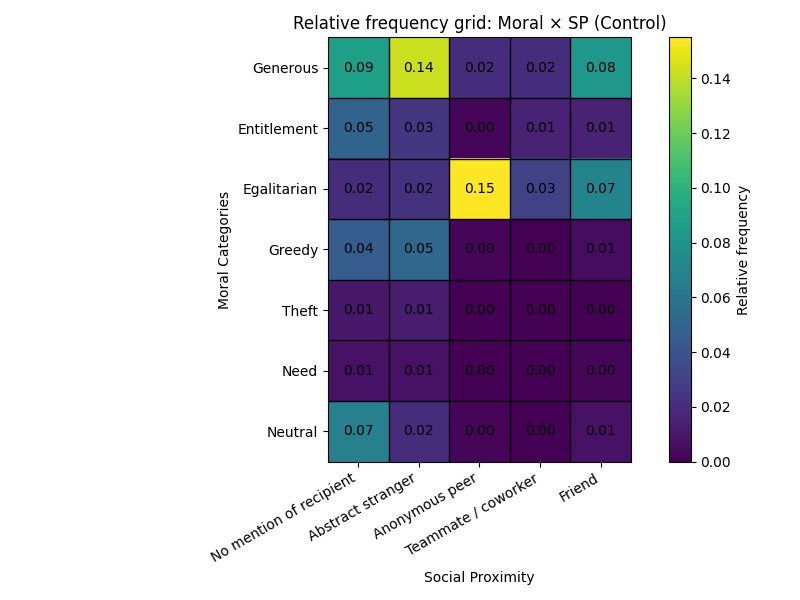
\includegraphics[width=\linewidth]{hp_sp_moral_corr_ctrl.png}
\caption{Joint distribution of social proximity and moral categories (hypothetical-allocation measure), Control.}
\label{fig:hp_sp_moral_ctrl}
\end{figure}

\begin{figure}[!htbp]
\centering
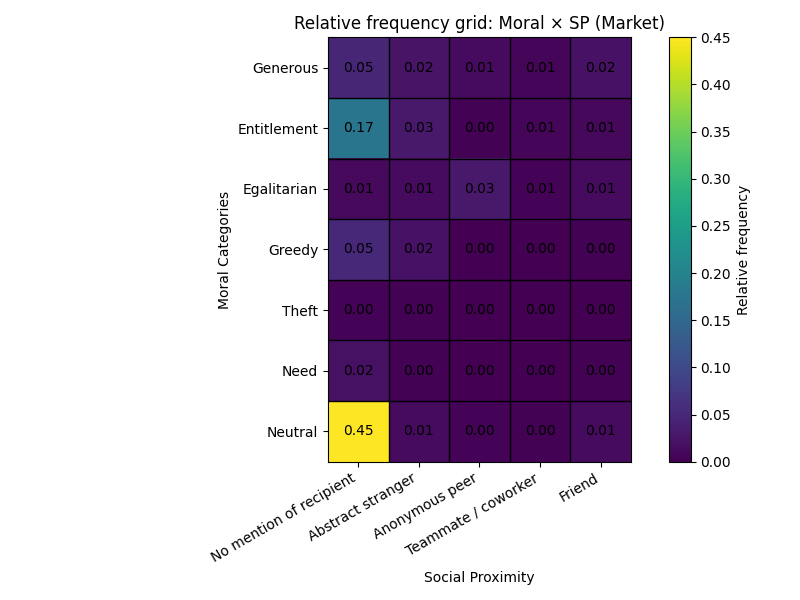
\includegraphics[width=\linewidth]{hp_sp_moral_corr_mkt.png}
\caption{Joint distribution of social proximity and moral categories (hypothetical-allocation measure), Market.}
\label{fig:hp_sp_moral_mkt}
\end{figure}

\clearpage

\section{Validation of the LLM Classification}
\label{app:validation}

Following the pre-registered procedure, the classification of the reasons question---produced by GPT-4.1 from a prompt containing the written classification rules---was validated against human coders. For each of the three classification batches---Player 1 in the story arms, Player 1 in Market and Control, and Player 2 in all four arms---two disjoint validation subsamples were drawn, stratified on the LLM-assigned category, and coded by hand by two research assistants, each responsible for one subsample throughout and blind to the treatment arm and to the game, using the same classification rules given to the LLM\@; in total, human coders classified 3,990 responses, and no response was coded in more than one subsample. Table~\ref{tab:llm_human_agreement} reports agreement rates and Cohen's $\kappa$ by batch, subsample, and arm. Agreement is high for Player 1's four-category scheme (three substantive categories plus the residual; 79--80\% pooled across subsamples, with $\kappa$ between 0.63 and 0.69) and lower for Player 2's finer five-category scheme (71\%, $\kappa=0.57$), where disagreements concentrate at the \emph{Moral good}/\emph{Mutual Benefit} boundary. The LLM labels in the validation subsamples coincide with the final classification used in the analysis files.
% RESOLVED 2026-07-10 (AA, round 3): protocol complete in the text above --- classifier GPT-4.1 with the written rules as prompt, two RA coders (one per subsample), blind to treatment arm and game, subsamples stratified on the LLM category. Blindness to the participant's chosen AMOUNT was never explicitly confirmed, so it is deliberately not claimed.

\begin{table}[!htbp]
\centering
\caption{\textbf{Validation of the LLM Classification Against Human Coders}}
\label{tab:llm_human_agreement}
\begin{tabular}{lcccccc}
\toprule
 & \multicolumn{3}{c}{Subsample 1} & \multicolumn{3}{c}{Subsample 2} \\
\cmidrule(lr){2-4} \cmidrule(lr){5-7}
 & $N$ & Agreement & $\kappa$ & $N$ & Agreement & $\kappa$ \\
\midrule
\multicolumn{7}{l}{\emph{Player 1, story conditions (Aid/Bonus)}} \\
\quad Bonus & 300 & 0.84 & 0.67 & 300 & 0.82 & 0.62 \\
\quad Aid & 300 & 0.81 & 0.65 & 300 & 0.76 & 0.56 \\
\quad All conditions & 600 & 0.82 & 0.66 & 600 & 0.79 & 0.59 \\
\addlinespace
\multicolumn{7}{l}{\emph{Player 1, Market/Control}} \\
\quad Control & 300 & 0.91 & 0.83 & 300 & 0.76 & 0.58 \\
\quad Market & 300 & 0.79 & 0.71 & 298 & 0.70 & 0.59 \\
\quad All conditions & 600 & 0.85 & 0.78 & 598 & 0.73 & 0.61 \\
\addlinespace
\multicolumn{7}{l}{\emph{Player 2, all conditions}} \\
\quad Control & 200 & 0.70 & 0.54 & 200 & 0.73 & 0.55 \\
\quad Market & 199 & 0.66 & 0.56 & 200 & 0.71 & 0.61 \\
\quad Bonus & 197 & 0.68 & 0.48 & 199 & 0.67 & 0.42 \\
\quad Aid & 197 & 0.72 & 0.58 & 200 & 0.81 & 0.69 \\
\quad All conditions & 793 & 0.69 & 0.55 & 799 & 0.73 & 0.59 \\
\addlinespace
\emph{Overall} & \multicolumn{6}{c}{$N=3,990$, agreement $=0.76$, $\kappa=0.64$} \\
\bottomrule
\end{tabular}
\begin{flushleft}
\footnotesize Notes: Human coders classified free-text answers to the reasons question using the same classification rules given to the LLM (GPT-4.1). Each batch comprises two disjoint validation subsamples drawn stratified on the LLM-assigned category (for Player 1, 100 responses per game--condition cell across DG-KW, UG, and TG\@; for Player 2, roughly 100 per game--condition cell across UG and TG in all four conditions); each subsample was coded by one of two research assistants, blind to the condition and to the game. Agreement is the share of responses assigned to the same category; $\kappa$ is Cohen's kappa over the full category set (four categories for Player 1, five for Player 2), including the residual ``No clear justification''.
\end{flushleft}
\end{table}


\clearpage

\section{Instructions and Stories}
\label{app:instructions}

This appendix reproduces the instructions for the main conditions as seen by participants (abridged; full screenshots available upon request) and the two stories.

\subsection{Dictator Game, Abstract Frame (KW)}

\begin{quote}\small
In this task, you are matched with another Prolific participant. You will never know the identity of the person with whom you are paired, and this person will never know your identity. You and your match are provisionally allocated a certain amount of dollars, adding to a total of \textbf{\$12}. You will have the chance to decide \textbf{whether and how to change this original allocation}.

The allocation chosen will be implemented for \textbf{1 participant out of 10}. This means that your decisions affect a bonus payment you and the other participant may receive. It is thus in your best interest to choose the allocations that you truly prefer.

[new page] You were provisionally allocated \textbf{\$12}. The other participant was provisionally allocated \textbf{\$0}. You have the option to make a transfer to the other participant. You can transfer any amount between \$0 and \$12.
\end{quote}

\subsection{Dictator Game, Abstract Frame (LT)}

\begin{quote}\small
[Same as above, then:] You were provisionally allocated \textbf{\$8}. The other participant was provisionally allocated \textbf{\$4}. You can transfer any amount between $-$\$4 and \$8. If you choose a negative dollar transfer to the other participant, this means that you take that amount \emph{from the other participant}.
\end{quote}

\subsection{Dictator Game, Market Frame (KW)}

\begin{quote}\small
In this task, you are matched with another Prolific participant. [\ldots] You take the role of \textbf{data provider (producer)}, and the other participant takes the role of \textbf{broker (intermediary)}. As a data provider, you produce survey data through online questionnaires like the one you are in. A computer will randomly determine an initial price for your data. You will then have the opportunity to \textbf{adjust this price} before it is sent to the broker.

The broker will sell your data to the research team for a fixed price of \$12. You will receive the final price you set. [\ldots] The \textbf{data provider (you)} receives a bonus payment equal to the final price you set. The \textbf{broker} receives \$12 from the research team for the sold data and pays the provider the set price, keeping the difference.

[new page] The computer selected a \textbf{starting price of \$12} for the data. You may change the price by any amount between $-$\$12 and \$0.
\end{quote}

\subsection{Ultimatum Game, Abstract Frame}

\begin{quote}\small
[\ldots] One of you will be assigned to be Player 1, and the other will be assigned to be Player 2. Player 1 is provisionally allocated \$12. \textbf{Player 1} will have the chance to decide \textbf{whether and how to change this original allocation}. After seeing the proposed allocation, \textbf{Player 2} will decide \textbf{whether to accept or reject it}. If Player 2 \textbf{accepts}, the proposed \textbf{allocation will be implemented}. If Player 2 \textbf{rejects}, \textbf{both players will receive \$0}.
\end{quote}

\subsection{Ultimatum Game, Market Frame}

\begin{quote}\small
[\ldots] One of you will be assigned to be \textbf{data provider (producer)}, and the other will be assigned to be \textbf{broker (intermediary)}. [\ldots] If you are assigned the role of \textbf{data provider}, you will have the opportunity to \textbf{adjust the initial price} before it is sent to the broker. The broker can sell the data to the research team for a fixed price of \textbf{\$12}. After seeing the proposed price set by the data provider, the \textbf{broker will decide whether to accept or reject it}. If the broker \textbf{accepts}, the data will be sold for \$12; the data provider receives a bonus equal to the final price set; the broker receives \$12 from the research team, pays the provider the set price, and keeps the difference. If the broker \textbf{rejects}, the sale does not take place and \textbf{both participants receive \$0}.
\end{quote}

\subsection{Trust Game, Abstract Frame}

\begin{quote}\small
[\ldots] \textbf{Player 1 will receive \$6}, and Player 2 will receive \$0. \textbf{Player 1} will decide \textbf{how much of the \$6 to send} to Player 2. \textbf{Any amount sent will be multiplied by 3} before being received by Player 2. After receiving this amount, \textbf{Player 2} will decide \textbf{how much of it to send back to Player 1}. The amount sent back will not be changed.
\end{quote}

\subsection{Trust Game, Market Frame}

\begin{quote}\small
[\ldots] The data provider has produced 6 units of data, each valued at \$1 by the research team, for a total of \$6. If you are assigned the role of data provider, you will decide how many units to sell to the research team for \$1 per unit, and how many units to transfer to the broker. The broker has access to a specialized buyer who is willing to pay \$3 per unit, so the broker's revenue is 3 times the number of units you send. After the sale, as a \textbf{broker you will decide whether and how much of the revenue to transfer back to the data provider}.
\end{quote}

\subsection{Stories}

\paragraph{Bonus.}
\begin{quote}\small\itshape
After weeks of intense preparation, Steve was thrilled to learn that his team was awarded a performance bonus for exceeding their sales target. The recognition felt satisfying---a tangible reward for the long hours he'd poured into work and the many nights he'd stayed late fine-tuning his pitch. The director called Steve to discuss the bonus and said: ``You guys did great. Since you are the team leader, the full bonus is allocated to you. However, you may choose to give a portion to your teammate Max if you wish. The final decision is yours.'' % chktex 38

Now Steve faced a choice. He could keep the full bonus, as initially allocated. Or he could give some to Max, knowing that Max made a significant contribution to the team's success. What should he do?
\end{quote}

\paragraph{Aid.}
\begin{quote}\small\itshape
James was going through a rough financial patch. He struggled to make ends meet and had no savings left. One morning, he received an unexpected email from a government welfare agency he had applied to months ago. ``Congratulations! You have been selected for financial assistance. You will be receiving the full aid amount to help with your expenses.'' % chktex 38

As James went to the agency to collect, he found Mark, a neighbor. He learned that Mark also applied but wasn't selected. Only James received the funds.

Now James faced a choice. Should he keep all the money for himself? James was tempted because he really needed the money, and Mark was just an acquaintance. Or should he give some of it to Mark, given that he was struggling? What should he do?
\end{quote}

\clearpage

\section{A Disparity-Based Alternative Model}
\label{app:theory_reconciliation}

Before adopting the model of Section~\ref{sec:model}, we developed a richer alternative in which the moral motive is outcome-based---a quadratic cost of the \emph{payoff disparity} $(y_S-y_R)^2$ rather than of the action's distance from the equal split---and beliefs are point forecasts of the receiver's attention weights (with \emph{projection}, forecasting the other with one's own weights, as a focal special case) rather than primitives of the representation. That model is developed in full, with proofs, norm-based trust-game variants, and robustness to concave utility, in a companion Model Appendix.
% TODO: decide whether to bundle the companion Model Appendix (currently working_docs/model_companion_disparity.pdf; NOT model.pdf, which is now the Model 2.0 note) as an online appendix to this paper.

The two models share the same motive triad---own earnings ($\sigma$ here, $\omega_o$ there), efficiency ($\rho-\sigma$ here, $\omega_e$ there), and a norm ($\mu$ here, disparity attention $\omega_d$ there)---and their core predictions coincide:
\begin{itemize}
\item \emph{Dictator game.} Transfers are capped at one half, decreasing in own-earnings attention, increasing in norm attention, with efficiency attention idle.
\item \emph{Ultimatum game.} Offers exceed dictator transfers for every attention profile, and category gaps compress relative to the dictator game because strategic discipline binds precisely on the senders whose own weights push offers down. The mechanics differ: censoring at a believed minimum acceptable offer there, a smooth acceptance schedule $p(t)$ here---the smooth version is what makes offers differentiable in beliefs and hence directly regression-interpretable.
\item \emph{Trust game.} Sending is driven by efficiency attention and gated by optimism about the return; purely material senders trust only above a break-even belief.
\end{itemize}

The differences are secondary but real. The disparity model produces kinked policy functions (intrinsic versus strategic offers; cautious versus full sending) where the present model produces smooth interior solutions; it ties receiver behavior to the same disparity weights that drive senders, where the present model founds the acceptance schedule on a protest benefit; and under projection it links beliefs to own weights mechanically, where the present model treats the believed behavior $\mathbf{x}$ as measured. On the one empirical pattern where the two disagreed in spirit---the disparity model, under projection, strained to match the ultimatum-game behavior of cooperative senders in the control sample---the present model is more comfortable, though the cooperative cell in the UG is small (3.3\% of classified responses) and neither model is sharply tested there.
% TODO (NG email): NG reads the disparity model's UG-control prediction for cooperative senders as hard to reconcile with the evidence; verify the exact comparison against Figure~\ref{fig:control_outcomes} cell means and state it precisely here.

For the exercises in this paper, nothing hinges on the choice: the comparative statics used to sign predictions in Sections~\ref{sec:treatment} and~\ref{sec:ge} agree across the two models. We use the action-norm model in the main text because it is simpler, because it integrates beliefs into the representation---which the belief data require---and because it turns the ultimatum and trust games into modified dictator games with one-line comparative statics.

\end{document}
